% Options for packages loaded elsewhere
\PassOptionsToPackage{unicode}{hyperref}
\PassOptionsToPackage{hyphens}{url}
%
\documentclass[
  ngerman,
]{article}
\usepackage{amsmath,amssymb}
\usepackage{lmodern}
\usepackage{iftex}
\ifPDFTeX
  \usepackage[T1]{fontenc}
  \usepackage[utf8]{inputenc}
  \usepackage{textcomp} % provide euro and other symbols
\else % if luatex or xetex
  \usepackage{unicode-math}
  \defaultfontfeatures{Scale=MatchLowercase}
  \defaultfontfeatures[\rmfamily]{Ligatures=TeX,Scale=1}
\fi
% Use upquote if available, for straight quotes in verbatim environments
\IfFileExists{upquote.sty}{\usepackage{upquote}}{}
\IfFileExists{microtype.sty}{% use microtype if available
  \usepackage[]{microtype}
  \UseMicrotypeSet[protrusion]{basicmath} % disable protrusion for tt fonts
}{}
\makeatletter
\@ifundefined{KOMAClassName}{% if non-KOMA class
  \IfFileExists{parskip.sty}{%
    \usepackage{parskip}
  }{% else
    \setlength{\parindent}{0pt}
    \setlength{\parskip}{6pt plus 2pt minus 1pt}}
}{% if KOMA class
  \KOMAoptions{parskip=half}}
\makeatother
\usepackage{xcolor}
\IfFileExists{xurl.sty}{\usepackage{xurl}}{} % add URL line breaks if available
\IfFileExists{bookmark.sty}{\usepackage{bookmark}}{\usepackage{hyperref}}
\hypersetup{
  pdftitle={Data Science für die Humangeographie: Ein pragmatischer Einstieg mit R},
  pdflang={de},
  hidelinks,
  pdfcreator={LaTeX via pandoc}}
\urlstyle{same} % disable monospaced font for URLs
\usepackage{color}
\usepackage{fancyvrb}
\newcommand{\VerbBar}{|}
\newcommand{\VERB}{\Verb[commandchars=\\\{\}]}
\DefineVerbatimEnvironment{Highlighting}{Verbatim}{commandchars=\\\{\}}
% Add ',fontsize=\small' for more characters per line
\usepackage{framed}
\definecolor{shadecolor}{RGB}{248,248,248}
\newenvironment{Shaded}{\begin{snugshade}}{\end{snugshade}}
\newcommand{\AlertTok}[1]{\textcolor[rgb]{0.94,0.16,0.16}{#1}}
\newcommand{\AnnotationTok}[1]{\textcolor[rgb]{0.56,0.35,0.01}{\textbf{\textit{#1}}}}
\newcommand{\AttributeTok}[1]{\textcolor[rgb]{0.77,0.63,0.00}{#1}}
\newcommand{\BaseNTok}[1]{\textcolor[rgb]{0.00,0.00,0.81}{#1}}
\newcommand{\BuiltInTok}[1]{#1}
\newcommand{\CharTok}[1]{\textcolor[rgb]{0.31,0.60,0.02}{#1}}
\newcommand{\CommentTok}[1]{\textcolor[rgb]{0.56,0.35,0.01}{\textit{#1}}}
\newcommand{\CommentVarTok}[1]{\textcolor[rgb]{0.56,0.35,0.01}{\textbf{\textit{#1}}}}
\newcommand{\ConstantTok}[1]{\textcolor[rgb]{0.00,0.00,0.00}{#1}}
\newcommand{\ControlFlowTok}[1]{\textcolor[rgb]{0.13,0.29,0.53}{\textbf{#1}}}
\newcommand{\DataTypeTok}[1]{\textcolor[rgb]{0.13,0.29,0.53}{#1}}
\newcommand{\DecValTok}[1]{\textcolor[rgb]{0.00,0.00,0.81}{#1}}
\newcommand{\DocumentationTok}[1]{\textcolor[rgb]{0.56,0.35,0.01}{\textbf{\textit{#1}}}}
\newcommand{\ErrorTok}[1]{\textcolor[rgb]{0.64,0.00,0.00}{\textbf{#1}}}
\newcommand{\ExtensionTok}[1]{#1}
\newcommand{\FloatTok}[1]{\textcolor[rgb]{0.00,0.00,0.81}{#1}}
\newcommand{\FunctionTok}[1]{\textcolor[rgb]{0.00,0.00,0.00}{#1}}
\newcommand{\ImportTok}[1]{#1}
\newcommand{\InformationTok}[1]{\textcolor[rgb]{0.56,0.35,0.01}{\textbf{\textit{#1}}}}
\newcommand{\KeywordTok}[1]{\textcolor[rgb]{0.13,0.29,0.53}{\textbf{#1}}}
\newcommand{\NormalTok}[1]{#1}
\newcommand{\OperatorTok}[1]{\textcolor[rgb]{0.81,0.36,0.00}{\textbf{#1}}}
\newcommand{\OtherTok}[1]{\textcolor[rgb]{0.56,0.35,0.01}{#1}}
\newcommand{\PreprocessorTok}[1]{\textcolor[rgb]{0.56,0.35,0.01}{\textit{#1}}}
\newcommand{\RegionMarkerTok}[1]{#1}
\newcommand{\SpecialCharTok}[1]{\textcolor[rgb]{0.00,0.00,0.00}{#1}}
\newcommand{\SpecialStringTok}[1]{\textcolor[rgb]{0.31,0.60,0.02}{#1}}
\newcommand{\StringTok}[1]{\textcolor[rgb]{0.31,0.60,0.02}{#1}}
\newcommand{\VariableTok}[1]{\textcolor[rgb]{0.00,0.00,0.00}{#1}}
\newcommand{\VerbatimStringTok}[1]{\textcolor[rgb]{0.31,0.60,0.02}{#1}}
\newcommand{\WarningTok}[1]{\textcolor[rgb]{0.56,0.35,0.01}{\textbf{\textit{#1}}}}
\usepackage{longtable,booktabs,array}
\usepackage{calc} % for calculating minipage widths
% Correct order of tables after \paragraph or \subparagraph
\usepackage{etoolbox}
\makeatletter
\patchcmd\longtable{\par}{\if@noskipsec\mbox{}\fi\par}{}{}
\makeatother
% Allow footnotes in longtable head/foot
\IfFileExists{footnotehyper.sty}{\usepackage{footnotehyper}}{\usepackage{footnote}}
\makesavenoteenv{longtable}
\usepackage{graphicx}
\makeatletter
\def\maxwidth{\ifdim\Gin@nat@width>\linewidth\linewidth\else\Gin@nat@width\fi}
\def\maxheight{\ifdim\Gin@nat@height>\textheight\textheight\else\Gin@nat@height\fi}
\makeatother
% Scale images if necessary, so that they will not overflow the page
% margins by default, and it is still possible to overwrite the defaults
% using explicit options in \includegraphics[width, height, ...]{}
\setkeys{Gin}{width=\maxwidth,height=\maxheight,keepaspectratio}
% Set default figure placement to htbp
\makeatletter
\def\fps@figure{htbp}
\makeatother
\setlength{\emergencystretch}{3em} % prevent overfull lines
\providecommand{\tightlist}{%
  \setlength{\itemsep}{0pt}\setlength{\parskip}{0pt}}
\setcounter{secnumdepth}{5}
\ifXeTeX
  % Load polyglossia as late as possible: uses bidi with RTL langages (e.g. Hebrew, Arabic)
  \usepackage{polyglossia}
  \setmainlanguage[]{german}
\else
  \usepackage[main=ngerman]{babel}
% get rid of language-specific shorthands (see #6817):
\let\LanguageShortHands\languageshorthands
\def\languageshorthands#1{}
\fi
\ifLuaTeX
  \usepackage{selnolig}  % disable illegal ligatures
\fi

\title{Data Science für die Humangeographie: Ein pragmatischer Einstieg mit R}
\usepackage{etoolbox}
\makeatletter
\providecommand{\subtitle}[1]{% add subtitle to \maketitle
  \apptocmd{\@title}{\par {\large #1 \par}}{}{}
}
\makeatother
\subtitle{Konzeption quantitativer Forschung}
\author{true}
\date{Winter- und Sommersemester 2020/21}

\begin{document}
\maketitle

{
\setcounter{tocdepth}{2}
\tableofcontents
}
\hypertarget{terminuxfcberblick}{%
\section*{Terminüberblick}\label{terminuxfcberblick}}
\addcontentsline{toc}{section}{Terminüberblick}

\emph{Alle Sitzungen finden von 13 bis 16h c.t. statt}

\begin{longtable}[]{@{}rrl@{}}
\toprule
Datum & Sitzung & Inhalt \\
\midrule
\endhead
2. November 2020 & 1 & \protect\hyperlink{vorbesprechung}{Vorbesprechung} \\
9. November 2020 & 2 & \protect\hyperlink{erste-schritte}{Erste Schritte} \\
16. November 2020 & 3 & \protect\hyperlink{text-anderson-2008}{Text: Anderson 2008} \\
23. November 2020 & 4 & \protect\hyperlink{datenstrukturen}{Datenstrukturen} \\
30. November 2020 & 5 & \protect\hyperlink{visualisierungen}{Visualisierungen} \\
7. Dezember 2020 & 6 & \protect\hyperlink{text-shelton-et-al.-2014}{Text: Shelton et al.~2014} \\
14. Dezember 2020 & 7 & \protect\hyperlink{geodaten}{Geodaten} \\
11. Januar 2021 & 8 & \protect\hyperlink{choroplethen}{Choroplethen} \\
18. Januar 2021 & 9 & \protect\hyperlink{text-chandra-2014}{Text: Chandra 2014} \\
25. Januar 2021 & 10 & \protect\hyperlink{html-tabellen}{HTML-Tabellen} \\
1. Februar 2021 & 11 & \protect\hyperlink{web-scraping}{Web scraping} \\
8. Februar 2021 & 12 & \protect\hyperlink{text-straube-2021}{Text: Straube 2021} \\
15. Februar 2021 & 13 & \protect\hyperlink{pruxe4sentationen}{Präsentationen} \\
\emph{31. März 2021} & & \emph{Abgabe Exposé} \\
12. April 2021 & 14 & \protect\hyperlink{apis}{APIs} \\
19. April 2021 & 15 & \protect\hyperlink{serialisierung}{Serialisierung} \\
26. April 2021 & 16 & \protect\hyperlink{text-breuer-2005}{Text: Breuer 2005} \\
3. Mai 2021 & 17 & {[}Reguläre Ausdrücke{]} \\
10. Mai 2021 & 18 & {[}Merging, Grouping{]} \\
17. Mai 2021 & 19 & {[}Text: Bowker und Star 2003{]} \\
\emph{24. Mai 2021} & 20 & \emph{Entfällt (Pfingstmontag)} \\
31. Mai 2021 & 21 & {[}Datenmanagement und Kollaboration{]} \\
7. Juni 2021 & 22 & {[}Clusteranalyse{]} \\
14. Juni 2021 & 23 & {[}Text: Beer 2017{]} \\
21. Juni 2021 & 24 & {[}ANOVA{]} \\
28. Juni 2021 & 25 & {[}Rmarkdown{]} \\
5. Juli 2021 & 26 & \protect\hyperlink{pruxe4sentationen}{Präsentationen} \\
12. Juli 2021 & 27 & \protect\hyperlink{pruxe4sentationen}{Präsentationen} \\
\bottomrule
\end{longtable}

\hypertarget{online-ressourcen}{%
\section*{Online-Ressourcen}\label{online-ressourcen}}
\addcontentsline{toc}{section}{Online-Ressourcen}

\hypertarget{r-tutorials-und-ebooks}{%
\subsection*{R Tutorials und eBooks}\label{r-tutorials-und-ebooks}}
\addcontentsline{toc}{subsection}{R Tutorials und eBooks}

\begin{itemize}
\item
  \textbf{R for Data Science}\\
  \url{https://r4ds.had.co.nz/}~\\
  Ausführliches Handbuch, Fokus auf Data Science
\item
  \textbf{RStudio Cloud Primers}\\
  \url{https://rstudio.cloud/learn/primers/1}
\item
  \textbf{Swirl}\\
  \url{https://swirlstats.com/students.html}~\\
  Interaktives Tutorial als R-Paket, mit verschiedenen Lektionen
\item
  \textbf{Quick-R}\\
  \url{https://www.statmethods.net/r-tutorial/index.html}~\\
  Überblickartiges Tutorial, kurz und bündig
\item
  \textbf{RStudio Cheat Sheets}\\
  \url{https://www.rstudio.com/resources/cheatsheets/}~\\
  Einseitige Cheat Sheets zu verschiedenen Themen
\item
  \textbf{Google's R Style Guide}\\
  \url{https://google.github.io/styleguide/Rguide.xml}~\\
  Regeln für leserlichen R Code
\end{itemize}

\hypertarget{inspiration-fuxfcr-visualisierungen}{%
\subsection*{Inspiration für Visualisierungen}\label{inspiration-fuxfcr-visualisierungen}}
\addcontentsline{toc}{subsection}{Inspiration für Visualisierungen}

\begin{itemize}
\item
  \textbf{R Graph Gallery}\\
  \url{https://www.r-graph-gallery.com/}~\\
  Viele Beispiele für verschiedenste Visualisierungen
\item
  \textbf{DDJ Katalog}\\
  \url{http://katalog.datenjournalismus.net/\#/}~\\
  Portfolio Datenjournalismus, leider etwas veraltet
\item
  \textbf{Subreddits}\\
  \url{https://www.reddit.com/r/dataisbeautiful}~\\
  \url{https://www.reddit.com/r/DataArt/}~\\
  \url{https://www.reddit.com/r/MapPorn/}
\item
  \textbf{Infographics}\\
  \url{https://www.listendata.com/2019/06/create-infographics-with-r.html}
\item
  \textbf{HTML Widgets für R}
  \url{http://gallery.htmlwidgets.org/}
\end{itemize}

\hypertarget{spezialthemen}{%
\subsection*{Spezialthemen}\label{spezialthemen}}
\addcontentsline{toc}{subsection}{Spezialthemen}

\begin{itemize}
\item
  \textbf{HTML-Überblick}\\
  \url{https://www.tutorialspoint.com/de/html/}
\item
  \textbf{Tutorial Reguläre Ausdrücke}\\
  \url{https://danielfett.de/en/tutorials/tutorial-regulare-ausdrucke/}~\\
  Deutschsprachige Einführung zu regulären Ausdrücken
\item
  \textbf{Übersicht CSS-Selektoren}\\
  \url{https://www.w3schools.com/cssref/css_selectors.asp}
\end{itemize}

\hypertarget{vorbesprechung}{%
\section{Vorbesprechung}\label{vorbesprechung}}

\hypertarget{uxfcberblick}{%
\subsection{Überblick}\label{uxfcberblick}}

\hypertarget{seminar-im-curriculum}{%
\subsubsection{Seminar im Curriculum}\label{seminar-im-curriculum}}

\begin{itemize}
\tightlist
\item
  Dieses Seminar ist Bestandteil des Moduls BA3.
\item
  Das Projektseminar besteht aus zwei Teilen über zwei Semester:

  \begin{itemize}
  \tightlist
  \item
    Konzeption quantitativer Forschung (Wintersemester)
  \item
    Analyse quantitativer Daten (Sommersemester)
  \end{itemize}
\item
  Im Winter gibt es \protect\hyperlink{terminuxfcberblick}{12 inhaltliche Termine} (davon 4x Textarbeit).
\item
  Im Sommer wird das Seminar mit den selben Teilnehmer*innen fortgeführt.
\end{itemize}

\hypertarget{lernziele-fuxfcr-das-wintersemester}{%
\subsubsection{Lernziele für das Wintersemester}\label{lernziele-fuxfcr-das-wintersemester}}

Sie können\ldots{}

\begin{itemize}
\tightlist
\item
  einfache Skripte in R eigenständig erstellen.
\item
  Datensätze in vielfältigen Formaten visualisieren.
\item
  Online-Ressourcen gezielt einsetzen.
\item
  Möglichkeiten der Datenbeschaffung identifizieren.
\item
  epistemologische Verschiebungen durch Data Science wiedergeben.
\end{itemize}

\hypertarget{technische-anforderungen}{%
\subsubsection{Technische Anforderungen}\label{technische-anforderungen}}

\begin{itemize}
\tightlist
\item
  Es sind keine Vorkenntnisse in R erforderlich.
\item
  Sie brauchen einen Laptop, mit dem Sie gut arbeiten können.
\item
  Wir benutzen die \href{https://rstudio.cloud}{RStudio Cloud} als Plattform.
\item
  Sie brauchen einen ruhigen Arbeitsplatz.
\end{itemize}

\hypertarget{unterstuxfctzung-im-corona-semester}{%
\subsubsection{Unterstützung im Corona-Semester}\label{unterstuxfctzung-im-corona-semester}}

\begin{itemize}
\tightlist
\item
  Die Uni bietet einen \href{https://www.starkerstart.uni-frankfurt.de/92914986/ContentPage_92914986}{``Semesterlaptop''} an.
\item
  Bei Bedarf kann ich gerne versuchen, Arbeitsplätze im Seminarraum (PEG) anzubieten.
\item
  Bitte kontaktieren Sie mich per E-Mail, falls Sie einen Arbeitsplatz regelmäßig in Anspruch nehmen wollen würden.
\end{itemize}

\hypertarget{seminarformat}{%
\subsection{Seminarformat}\label{seminarformat}}

\begin{itemize}
\tightlist
\item
  Das Seminar findet jede Woche Montags, 13--16h c.t. statt.
\item
  Der Zoom-Link, den Sie per E-Mail erhalten haben, bleibt gleich.
\item
  Wir machen um ca. 14:25h eine zehnminütige Pause.
\item
  Für Textbesprechungen wird die Gruppe zweigeteilt.
\item
  Dieses Seminar findet in verschiedenen Modi statt:
\end{itemize}

\hypertarget{input-und-plenum}{%
\subsubsection{Input und Plenum}\label{input-und-plenum}}

\begin{itemize}
\tightlist
\item
  Ich rede oder moderiere (mit Folien oder ohne)
\item
  Sie hören mir und Ihren Kommiliton*innen aufmerksam zu
\item
  Sie ``melden'' sich für Redebeiträge oder Fragen (Zoom-Funktion)
\item
  Die*der Chat-Verantwortliche unterbricht mich bei Klärungsbedarf
\end{itemize}

\hypertarget{think-pair-share}{%
\subsubsection{Think-pair-share}\label{think-pair-share}}

\begin{itemize}
\tightlist
\item
  Sie bearbeiten eine Fragestellung in zufälligen Zweier-Konstellationen (Breakout-Session)
\item
  Nach einer vorgegebenen Zeitspanne kehren Sie ins Plenum zurück
\item
  Ich fordere Sie ggf. auf, Ergebnisse und offene Fragen mit der Gruppe zu teilen
\end{itemize}

\hypertarget{follow-the-recipe}{%
\subsubsection{Follow the recipe}\label{follow-the-recipe}}

\begin{itemize}
\tightlist
\item
  Ich teile ein unvollständiges Beispielprojekt.
\item
  Wir gehen die Teilschritte nach und nach durch.
\item
  Ich ``habe den Plan'', stelle aber immer wieder Fragen ans Plenum.
\item
  Sie vollziehen die Schritte an Ihrer eigenen Kopie des Projekts nach.
\item
  Die*der Chat-Verantwortliche unterbricht mich bei Klärungsbedarf
\end{itemize}

\hypertarget{hands-on-session}{%
\subsubsection{Hands-on session}\label{hands-on-session}}

\begin{itemize}
\tightlist
\item
  Sie bearbeiten praktische Aufgabenstellungen alleine.
\item
  Dabei sind sie in zufälligen Dreier-Konstellationen (Breakout-Session).
\item
  Bei Fragen oder Problemen wenden Sie sich zunächst an Ihre Kleingruppe.
\item
  Falls Sie nicht weiterkommen, fordern Sie Hilfe an (Zoom-Funktion).
\item
  Ich reagiere auf Hilfegesuche oder schaue in zufälligen Gruppen vorbei.
\end{itemize}

\hypertarget{share-your-work}{%
\subsubsection{Share your work}\label{share-your-work}}

\begin{itemize}
\tightlist
\item
  Ich wähle eine Teilnehmer*in zufällig aus.
\item
  Die Person teilt ihren Bildschirm und berichtet von ihrer Bearbeitung eines Problems.
\item
  Alle anderen unterstützen solidarisch durch aktives Nachvollziehen, Nachfragen und Hinweise.
\end{itemize}

\hypertarget{leistungsnachweise}{%
\subsection{Leistungsnachweise}\label{leistungsnachweise}}

\hypertarget{exposuxe9-wise}{%
\subsubsection{Exposé (WiSe)}\label{exposuxe9-wise}}

\begin{itemize}
\tightlist
\item
  Zum Ende des Wintersemesters geben Sie ein Exposé für ein Untersuchungsvorhaben für das Sommersemester ab.
\item
  Sie können sich mit bis zu vier Personen zusammenschließen.
\item
  Die Projektgruppe besteht dann verbindlich für das Sommersemester.
\item
  Damit steigen aber auch die Anforderungen an Umfang, Detail und technischen Anspruch.
\item
  Umfang für das Exposé: max. 15k Zeichen inkl. Leerzeichen, exkl. Literaturverzeichnis
\item
  Als Abgabetermin haben wir den 31. März vereinbart.
\end{itemize}

\hypertarget{inhalte}{%
\paragraph{Inhalte}\label{inhalte}}

\begin{itemize}
\tightlist
\item
  Einführung ins Thema
\item
  Forschungsstand / Literaturüberblick
\item
  Herleitung einer klar abgegrenzten (vorläufigen) Forschungsfrage
\item
  Konkrete Datenquellen
\item
  Ideen für Verfahren und Visualisierungen
\end{itemize}

\hypertarget{bewertungskriterien}{%
\paragraph{Bewertungskriterien}\label{bewertungskriterien}}

Alle Kriterien werden mit einer (runden) Schulnote bewertet. Der gewichtete Schnitt ergibt die Gesamtnote.

\begin{longtable}[]{@{}
  >{\raggedright\arraybackslash}p{(\columnwidth - 4\tabcolsep) * \real{0.28}}
  >{\raggedleft\arraybackslash}p{(\columnwidth - 4\tabcolsep) * \real{0.12}}
  >{\raggedright\arraybackslash}p{(\columnwidth - 4\tabcolsep) * \real{0.60}}@{}}
\toprule
Kriterium & Gewichtung & Erläuterung \\
\midrule
\endhead
Ziterweise und Formatierung & 10\% & Der Text erfüllt formale Anforderungen an Wissenschaftlichkeit. \\
Ausdruck und Rechtschreibung & 10\% & Der Text ist sprachlich gelungen. \\
Roter Faden & 10\% & Der Text ist übersichtlich strukturiert und die Einzelteile greifen gut ineinander. \\
Literatur & 10\% & Die zitierten Quellen sind für eine Einführung ins Thema geeignet und werden gut zusammengefasst. \\
Theorie & 10\% & Relevante wissenschaftliche Perspektiven werden anhand von geeigneter Fachliteratur aufgezeigt. \\
Fragestellung & 10\% & Die Forschungsfrage ist für das Vorhaben geeignet und wird überzeugend hergeleitet. \\
Datenquellen & 20\% & Die Datenquellen sind geeignet und detailliert beschrieben. \\
Design & 20\% & Das Untersuchungsvorhaben ist nachvollziehbar beschrieben, und der technische Anspruch ist dem Projektseminar angemessen. \\
\bottomrule
\end{longtable}

\hypertarget{projektbericht-sose}{%
\subsubsection{Projektbericht (SoSe)}\label{projektbericht-sose}}

\begin{itemize}
\tightlist
\item
  Zum Ende des Sommersemesters geben Sie einen Projektbericht ab.
\item
  Der Projektbericht darf (überarbeitete) Teile des Exposés enthalten.
\item
  Die Gruppen, in denen Sie Ihr Exposé verfasst haben, bleiben verbindlich bestehen.
\item
  Umfang für den Projektbericht:

  \begin{itemize}
  \tightlist
  \item
    max. 35k Zeichen
  \item
    inkl. Leerzeichen
  \item
    exkl. Literaturverzeichnis
  \item
    exkl. Code
  \end{itemize}
\item
  Als Abgabetermin haben wir den 31. August vereinbart.
\end{itemize}

\hypertarget{format}{%
\paragraph{Format}\label{format}}

\begin{itemize}
\tightlist
\item
  Der Projektbericht muss in Rmarkdown verfasst werden und (grundsätzlich) ausführbar sein.

  \begin{itemize}
  \tightlist
  \item
    Daten, die für die Ausführung benötigt werden, müssen mit abgegeben werden. (Bei sehr großen Datensätzen wenden Sie sich bitte frühzeitig an mich).
  \item
    Dabei dürfen alle Pakete aus CRAN verwendet werden. Eigene Scripts müssen mit abgegeben werden.
  \item
    Aufwändige oder prekäre Zwischenschritte (etwa Web Scraping, rechenintensive Grafiken) bitte als Zwischenergebnis speichern. (Code trotzdem darlegen!)
  \end{itemize}
\end{itemize}

\hypertarget{inhalte-1}{%
\paragraph{Inhalte}\label{inhalte-1}}

\begin{itemize}
\tightlist
\item
  Einführung ins Thema
\item
  Forschungsstand / Literaturüberblick
\item
  Herleitung einer klar abgegrenzten Forschungsfrage
\item
  Besprechung der Datenquellen
\item
  Darstellung der Methoden für

  \begin{itemize}
  \tightlist
  \item
    Datenbeschaffung
  \item
    Datenaufbereitung (säubern, verschneiden)
  \item
    Datenanalyse (Visualisierung, statische Verfahren)
  \end{itemize}
\item
  Präsentation der Ergebnisse
\item
  Einordnung der Ergebnisse
\end{itemize}

\hypertarget{bewertungskriterien-1}{%
\paragraph{Bewertungskriterien}\label{bewertungskriterien-1}}

Alle Kriterien werden mit einer (runden) Schulnote bewertet. Der gewichtete Schnitt ergibt die Gesamtnote.

\begin{longtable}[]{@{}
  >{\raggedright\arraybackslash}p{(\columnwidth - 4\tabcolsep) * \real{0.28}}
  >{\raggedleft\arraybackslash}p{(\columnwidth - 4\tabcolsep) * \real{0.12}}
  >{\raggedright\arraybackslash}p{(\columnwidth - 4\tabcolsep) * \real{0.60}}@{}}
\toprule
Kriterium & Gewichtung & Erläuterung \\
\midrule
\endhead
Ziterweise und Formatierung & 10\% & Der Text erfüllt formale Anforderungen an Wissenschaftlichkeit. \\
Ausdruck und Rechtschreibung & 10\% & Der Text ist sprachlich gelungen. \\
Roter Faden & 10\% & Der Text ist übersichtlich strukturiert und die Einzelteile greifen gut ineinander. \\
Literatur & 5\% & Die zitierten Quellen sind für eine Einführung ins Thema geeignet und werden gut zusammengefasst. \\
Theorie & 10\% & Relevante wissenschaftliche Perspektiven werden anhand von geeigneter Fachliteratur aufgezeigt. \\
Fragestellung & 5\% & Die Forschungsfrage ist für das Vorhaben geeignet und wird überzeugend hergeleitet. \\
Anspruch & 20\% & Der technische Anspruch ist dem Projektseminar angemessen. \\
Beschaffung & 10\% & Die Datenquellen sind geeignet und werden nachvollziehbar ausgelesen. \\
Aufbereitung & 10\% & Die Datenaufbereitung ist sauber durchgeführt und gut nachvollziehbar. \\
Analyse & 10\% & Die Datenanalyse ist geeignet, sauber durchgeführt und anschaulich beschrieben. \\
\bottomrule
\end{longtable}

\hypertarget{anwesenheit}{%
\subsubsection{Anwesenheit}\label{anwesenheit}}

\begin{itemize}
\tightlist
\item
  Es besteht Anwesenheitspflicht.
\item
  Für Ihre ersten zwei Fehltermine pro Semester brauche ich keine Entschuldigung (aber Sie sollten das ggf. mit ihrer Projektgruppe absprechen).
\item
  Sie sind dann selbstständig für die Nacharbeit der behandelten Themen zuständig.
\item
  Im Falle eines zusätzlichen Fehltermins brauche ich ein Attest und einen Nachweis über Nacharbeit.
\item
  Zur Anwesenheit gehört\ldots{}

  \begin{itemize}
  \tightlist
  \item
    uneingeschränkte Aufmerksamkeit über die komplette Veranstaltungsdauer,
  \item
    aktive Mitarbeit an Beispielen,
  \item
    Bearbeitung von Übungsaufgaben,
  \item
    aktive Beteiligung an Diskussionen.
  \end{itemize}
\item
  Eine eingeschaltete Kamera macht das allen Beteiligten leichter!
\end{itemize}

\hypertarget{lehrphilosophie}{%
\subsection{Lehrphilosophie}\label{lehrphilosophie}}

\begin{itemize}
\tightlist
\item
  Die folgenden vier ``Säulen'' habe ich mal im Rahmen einer Fortbildung als meine ``Lehrphilosophie'' definiert.
\item
  Sie spiegeln meinen eigenen Anspruch an meine Lehre wider und sind auch als Vorschlag für ein gutes Miteinander zu verstehen.
\item
  Begreifen Sie die hier genannten Aspekte gerne auch als Ermunterung, sie von mir und Ihren Kommiliton*innen einzufordern, wenn sie in der Veranstaltung zu kurz kommen.
\end{itemize}

\hypertarget{transparenz}{%
\subsubsection{Transparenz}\label{transparenz}}

\begin{itemize}
\tightlist
\item
  Erforderliche Leistungen und Bewertungskriterien sind vorab bekannt.
\item
  Termine und Regelungen werden in der Vorbereitungssitzung verbindlich vereinbart.
\item
  Aktuelle Lehrmaterialien stehen online durchgängig zur Verfügung.
\end{itemize}

\hypertarget{praktische-uxfcbungen}{%
\subsubsection{Praktische Übungen}\label{praktische-uxfcbungen}}

\begin{itemize}
\tightlist
\item
  Eigenständige Anwendung steht im Vordergrund.
\item
  Verfahren und Techniken werden mit Beispielen und Übungen erarbeitet.
\item
  Die perfekte Aufgabe ist immer ein bisschen ``zu schwer''.
\item
  Toleranz für Frustration ist eine wichtige Fähigkeit und lässt sich trainieren.
\end{itemize}

\hypertarget{geschuxfctzte-ruxe4ume}{%
\subsubsection{Geschützte Räume}\label{geschuxfctzte-ruxe4ume}}

\begin{itemize}
\tightlist
\item
  Alle können sich im Plenum respektiert und sicher fühlen. Verletzendes Verhalten wird benannt.
\item
  Es gibt einen vertrauensvollen Rahmen für ehrlichen Austausch.
\item
  Frustrationen und Momente des Scheiterns werden ernst genommen und konstruktiv bearbeitet.
\end{itemize}

\hypertarget{kritische-reflexion}{%
\subsubsection{Kritische Reflexion}\label{kritische-reflexion}}

\begin{itemize}
\tightlist
\item
  Auch Teilnehmende, die kein weiterführendes Interesse an der Anwendung quantitativer Verfahren haben, sind im Seminar gut aufgehoben.
\item
  Verfahren werden kontextualisiert, ihre Limitationen werden aufgezeigt.
\item
  Kritische Forschung zu quantitativen Praktiken wird besprochen.
\end{itemize}

\hypertarget{erste-schritte}{%
\section{Erste Schritte}\label{erste-schritte}}

\hypertarget{vorbereitung}{%
\subsection{Vorbereitung}\label{vorbereitung}}

\begin{itemize}
\tightlist
\item
  Machen Sie sich einen kostenlosen Account auf \url{https://rstudio.cloud}
\item
  Treten Sie dem Seminar-Workspace bei. (Sie erhalten eine Einladung per E-Mail.)
\item
  Optional/alternativ: installieren Sie \href{https://www.r-project.org/}{R} und \href{https://rstudio.com/}{RStudio} auf Ihrem Computer.
\end{itemize}

\hypertarget{lernziele-fuxfcr-diese-sitzung}{%
\subsection{Lernziele für diese Sitzung}\label{lernziele-fuxfcr-diese-sitzung}}

Sie können\ldots{}

\begin{itemize}
\tightlist
\item
  Rechenoperatoren einsetzen.
\item
  Variablen zuweisen.
\item
  Funktionen aufrufen.
\item
  Hilfe zu Funktionen anzeigen.
\item
  die wichtigsten Variablentypen bestimmen.
\item
  zwischen Variablentypen konvertieren.
\end{itemize}

\hypertarget{operatoren}{%
\subsection{Operatoren}\label{operatoren}}

Zunächst stellen wir fest, dass man die R-Konsole ganz banal als Taschenrechner benutzen kann:

\begin{Shaded}
\begin{Highlighting}[]
\DecValTok{1} \SpecialCharTok{+} \DecValTok{4}
\DocumentationTok{\#\# [1] 5}
\DecValTok{8} \SpecialCharTok{/} \DecValTok{3}
\DocumentationTok{\#\# [1] 2.666667}
\NormalTok{(}\FloatTok{2.45} \SpecialCharTok{+} \FloatTok{3.5}\NormalTok{) }\SpecialCharTok{*} \DecValTok{7}
\DocumentationTok{\#\# [1] 41.65}
\end{Highlighting}
\end{Shaded}

Die Zeichen \texttt{+}, \texttt{-}, \texttt{*} usw. heißen in der Informatik Operatoren oder Infixe (weil sie immer zwischen zwei Werten stehen).

\hypertarget{variablen}{%
\subsection{Variablen}\label{variablen}}

Variablen funktionieren so, dass man einem \emph{Wert} einen Namen gibt. Die Zuweisung folgt dabei dem Schema \texttt{NAME\ \textless{}-\ WERT}:

\begin{Shaded}
\begin{Highlighting}[]
\NormalTok{x }\OtherTok{\textless{}{-}} \DecValTok{5}
\end{Highlighting}
\end{Shaded}

Nach einer erfolgreichen Variablenzuweisung gibt die Konsole \emph{keine} Rückmeldung, sondern nur bei Fehlern.

\texttt{x} steht jetzt für die Zahl fünf. Mit dieser Variable können wir jetzt genauso rechnen wie mit einer Zahl:

\begin{Shaded}
\begin{Highlighting}[]
\NormalTok{x }\SpecialCharTok{+} \DecValTok{3}
\DocumentationTok{\#\# [1] 8}
\end{Highlighting}
\end{Shaded}

Auch die Zuweisung von Variablen kann Rechenoperationen und andere Variablen enthalten:

\begin{Shaded}
\begin{Highlighting}[]
\NormalTok{y }\OtherTok{\textless{}{-}}\NormalTok{ (x }\SpecialCharTok{*} \DecValTok{2}\NormalTok{) }\SpecialCharTok{{-}} \DecValTok{1}
\FunctionTok{print}\NormalTok{(y)}
\DocumentationTok{\#\# [1] 9}
\end{Highlighting}
\end{Shaded}

Der Befehl \texttt{print(y)} ist dabei ganz einfach die Anweisung an die Konsole, den Wert für \texttt{y} auszugeben. Das passiert zwar auch, wenn man nur \texttt{y} eingibt, aber \texttt{print(y)} (oder \texttt{print(x)}, \texttt{print(1\ +\ 1)}, usw.) ist die formal korrekte Schreibweise.

Der Wert einer Variable kann auch verändert werden. Dafür weisen wir ihr einfach einen neuen Wert zu:

\begin{Shaded}
\begin{Highlighting}[]
\NormalTok{x }\OtherTok{\textless{}{-}} \DecValTok{20}
\FunctionTok{print}\NormalTok{(x)}
\DocumentationTok{\#\# [1] 20}
\end{Highlighting}
\end{Shaded}

Eine Besonderheit ist, dass der alte Wert der Variable auch innerhalb der Zuweisung eines neuen Werts benutzt werden darf. Das kann in einem Script sehr praktisch sein. Wenn wir \texttt{x} also um 0,5 erhöhen wollen, sieht das so aus:

\begin{Shaded}
\begin{Highlighting}[]
\NormalTok{x }\OtherTok{\textless{}{-}}\NormalTok{ x }\SpecialCharTok{+} \FloatTok{0.5}
\FunctionTok{print}\NormalTok{(x)}
\DocumentationTok{\#\# [1] 20.5}
\end{Highlighting}
\end{Shaded}

Dabei wird als Dezimaltrennzeichen ausschließlich der Punkt verwendet.

\hypertarget{konstanten}{%
\subsection{Konstanten}\label{konstanten}}

Manche benannten Werte sind schon in R eingebaut:

\begin{Shaded}
\begin{Highlighting}[]
\FunctionTok{print}\NormalTok{(pi)}
\DocumentationTok{\#\# [1] 3}
\end{Highlighting}
\end{Shaded}

Diese Werte heißen üblicherweise ``Konstanten'' -- allerdings lassen sie sich in R auch überschreiben!

\begin{Shaded}
\begin{Highlighting}[]
\NormalTok{pi }\OtherTok{\textless{}{-}} \DecValTok{3}
\FunctionTok{print}\NormalTok{(pi)}
\DocumentationTok{\#\# [1] 3}
\end{Highlighting}
\end{Shaded}

\hypertarget{funktionen}{%
\subsection{Funktionen}\label{funktionen}}

Mit \texttt{print()} haben wir schon unsere erste \emph{Funktion} kennengelernt. R stellt uns eine Vielzahl von verschiedenen Funktionen zur Verfügung, und sie werden immer nach dem gleichen Schema benutzt: \texttt{FUNKTIONSNAME(PARAMETER)}.

\emph{Parameter} (auf Englisch auch ``arguments'') sind die Werte, die als Input an die Funktion übergeben werden. Je nach Funktion können das auch mehrere Werte sein, die dann durch Kommas getrennt werden. So nimmt die Funktion \texttt{max()}, die den Maximalwert bestimmt, beliebig viele Zahlen als Parameter:

\begin{Shaded}
\begin{Highlighting}[]
\FunctionTok{max}\NormalTok{(}\DecValTok{1}\NormalTok{, }\DecValTok{2}\NormalTok{, }\DecValTok{2}\NormalTok{, }\DecValTok{5}\NormalTok{, }\DecValTok{4}\NormalTok{, }\DecValTok{3}\NormalTok{)}
\DocumentationTok{\#\# [1] 5}
\end{Highlighting}
\end{Shaded}

Die Funktion \texttt{round()} hat als optionalen Parameter die Anzahl der Nachkommastellen, auf die gerundet werden soll. Wenn er nicht angegeben wird, nimmmt dieser Parameter immer den Wert 0 an:

\begin{Shaded}
\begin{Highlighting}[]
\FunctionTok{round}\NormalTok{(}\FloatTok{4.567}\NormalTok{)}
\DocumentationTok{\#\# [1] 5}
\end{Highlighting}
\end{Shaded}

Aber er lässt sich auch spezifizieren:

\begin{Shaded}
\begin{Highlighting}[]
\FunctionTok{round}\NormalTok{(}\FloatTok{4.567}\NormalTok{, }\AttributeTok{digits =} \DecValTok{2}\NormalTok{)}
\DocumentationTok{\#\# [1] 4.57}
\end{Highlighting}
\end{Shaded}

Dabei sind die folgenden Ausdrücke identisch:

\begin{Shaded}
\begin{Highlighting}[]
\FunctionTok{round}\NormalTok{(}\FloatTok{4.567}\NormalTok{, }\AttributeTok{digits =} \DecValTok{2}\NormalTok{)}
\DocumentationTok{\#\# [1] 4.57}
\FunctionTok{round}\NormalTok{(}\FloatTok{4.567}\NormalTok{, }\DecValTok{2}\NormalTok{)}
\DocumentationTok{\#\# [1] 4.57}
\FunctionTok{round}\NormalTok{(}\AttributeTok{digits =} \DecValTok{2}\NormalTok{, }\FloatTok{4.567}\NormalTok{)}
\DocumentationTok{\#\# [1] 4.57}
\end{Highlighting}
\end{Shaded}

Was Funktionen genau machen und welche Parameter sie dabei nehmen, ist in der R-Dokumentation sehr ausführlich (und auf den ersten Blick recht kompliziert) beschrieben. Ganz am Ende der Hilfeseite finden sich oft Beipsiele. Die Hilfe zu einer Funktion kann mit folgendem Befehl aufgerufen werden:

\begin{Shaded}
\begin{Highlighting}[]
\NormalTok{?max}
\end{Highlighting}
\end{Shaded}

Notiz am Rande: Auch die Infix-Operatoren \texttt{+}, \texttt{-}, \texttt{*}, usw. sind eigentlich nur verkürzte Schreibweisen von Funktionen. Mit ``backticks'' ( ` ) lassen sie sich in vollwertige Funktionen zurückverwandeln:

\begin{Shaded}
\begin{Highlighting}[]
\StringTok{\textasciigrave{}}\AttributeTok{+}\StringTok{\textasciigrave{}}\NormalTok{(}\DecValTok{2}\NormalTok{, }\DecValTok{2}\NormalTok{)}
\DocumentationTok{\#\# [1] 4}
\end{Highlighting}
\end{Shaded}

\hypertarget{strings}{%
\subsection{Strings}\label{strings}}

R kann nicht nur mit Zahlen umgehen, sondern auch mit Text. Ein \emph{String} ist eine Aneinanderreihung von Buchstaben, und wird mit einfachen oder doppelten Anführungszeichen umschlossen:

\begin{Shaded}
\begin{Highlighting}[]
\FunctionTok{print}\NormalTok{(}\StringTok{"Hello, World!"}\NormalTok{)}
\DocumentationTok{\#\# [1] "Hello, World!"}
\end{Highlighting}
\end{Shaded}

Auch Variablen können Strings als Wert haben:

\begin{Shaded}
\begin{Highlighting}[]
\NormalTok{name }\OtherTok{\textless{}{-}} \StringTok{"Hase"}
\end{Highlighting}
\end{Shaded}

Es gibt auch Funktionen, die Strings als Parameter nehmen. \texttt{paste} fügt Strings aneinander:

\begin{Shaded}
\begin{Highlighting}[]
\FunctionTok{paste}\NormalTok{(}\StringTok{"Mein Name ist"}\NormalTok{, name)}
\DocumentationTok{\#\# [1] "Mein Name ist Hase"}
\end{Highlighting}
\end{Shaded}

\hypertarget{datentypen}{%
\subsection{Datentypen}\label{datentypen}}

Den \emph{Typ} einer Variable oder eines Wertes bestimmen wir durch den Befehl \texttt{str()}:

\begin{Shaded}
\begin{Highlighting}[]
\FunctionTok{str}\NormalTok{(name)}
\DocumentationTok{\#\#  chr "Hase"}
\FunctionTok{str}\NormalTok{(}\DecValTok{10}\NormalTok{)}
\DocumentationTok{\#\#  num 10}
\end{Highlighting}
\end{Shaded}

Dabei steht \texttt{chr} („character``) für Strings und \texttt{num} („numeric``) für Zahlen.

Ein weiterer Variablentyp ist \texttt{logi} („logical``), der prinzipiell nur die Werte \texttt{TRUE} oder \texttt{FALSE} annehmen kann. Dieser Typ heißt auch \href{https://de.wikipedia.org/wiki/Boolesche_Variable}{Boolsche Variabel}:

\begin{Shaded}
\begin{Highlighting}[]
\FunctionTok{str}\NormalTok{(}\ConstantTok{FALSE}\NormalTok{)}
\DocumentationTok{\#\#  logi FALSE}
\end{Highlighting}
\end{Shaded}

Soweit es ein eindeutiges Ergebnis gibt, kann R mit den entsprechenden Befehlen Werte vom einen in den anderen Typ umwandeln:

\begin{Shaded}
\begin{Highlighting}[]
\FunctionTok{as.numeric}\NormalTok{(}\StringTok{"1000"}\NormalTok{)}
\DocumentationTok{\#\# [1] 1000}
\FunctionTok{as.character}\NormalTok{(x)}
\DocumentationTok{\#\# [1] "20.5"}
\FunctionTok{as.logical}\NormalTok{(}\DecValTok{0}\NormalTok{)}
\DocumentationTok{\#\# [1] FALSE}
\end{Highlighting}
\end{Shaded}

Kann R einen Wert nicht umwandeln, dann kommt dabei \texttt{NA} raus (mit einer Warnung):

\begin{Shaded}
\begin{Highlighting}[]
\FunctionTok{as.numeric}\NormalTok{(}\StringTok{"Hallo!"}\NormalTok{)}
\DocumentationTok{\#\# [1] NA}
\end{Highlighting}
\end{Shaded}

\texttt{NA} („not available/assigned``) ist dabei ein besonderer Wert, den jeder Variablentyp annehmen kann.

\hypertarget{aufgaben}{%
\subsection{Aufgaben}\label{aufgaben}}

\hypertarget{rechnen}{%
\subsubsection{Rechnen}\label{rechnen}}

Lösen Sie folgende Rechenaufgaben mit Hilfe von R:

\begin{itemize}
\tightlist
\item
  4 plus 10
\item
  8 mal 12
\item
  4 minus 7
\item
  3 hoch 18
\item
  4,5 geteilt durch die Summe von 5 und 8
\item
  Quadratwurzel aus 101
\item
  Kubikwurzel aus 12
\end{itemize}

\hypertarget{variablen-1}{%
\subsubsection{Variablen}\label{variablen-1}}

Weisen Sie den Variablen a bis g folgende Werte zu:

\begin{enumerate}
\def\labelenumi{\alph{enumi})}
\tightlist
\item
  TRUE
\item
  2
\item
  Ihren Namen
\item
  Die Quadratwurzel aus b
\item
  8 \(\textstyle\frac{1}{4}\)
\item
  Das vierfache von e
\item
  Die aktuelle Uhrzeit mit Datum und Zeitzone (automatisch generiert)
\end{enumerate}

\hypertarget{datentypen-1}{%
\subsubsection{Datentypen}\label{datentypen-1}}

Bestimmen Sie die Typen der Variablen a bis g.

Finden Sie je zwei Beispiele für die Umwandlung\ldots{}

\begin{itemize}
\tightlist
\item
  von \texttt{numeric} zu \texttt{character}
\item
  von \texttt{numeric} zu \texttt{logical}
\item
  von \texttt{character} zu \texttt{logical}
\item
  von \texttt{character} zu \texttt{numeric}
\item
  von \texttt{logical} zu \texttt{character}
\item
  von \texttt{logical} zu \texttt{numeric}
\item
  von \texttt{character} zu \texttt{Date}
\item
  von \texttt{Date} zu \texttt{numeric}
\end{itemize}

(\texttt{Date} ist kein eigentlicher Datentyp, aber erfüllt an dieser Stelle denselben Zweck.)

\hypertarget{swirl}{%
\subsubsection{Swirl}\label{swirl}}

Folgen Sie den Anleitungen, um Swirl zu installieren: \url{https://swirlstats.com/students.html}

Absolvieren Sie Lektion 1 („Basic Building Blocks``).

\hypertarget{recherche}{%
\subsubsection{Recherche}\label{recherche}}

Recherchieren Sie:

\begin{itemize}
\tightlist
\item
  Welche Funktion gibt den absoluten Wert einer Zahl aus? (z.B. -4 ergibt 4, 8 ergibt 8)
\item
  Welche Konstanten sind in R „eingebaut``?
\item
  Wie bestimmt man den „Rest`` einer Division? (z.B. 40 geteilt durch 7 hat den Rest 5)
\item
  In der Statistik wird zwischen stetigen und diskreten Variablen unterschieden. Welche äquivalente Unterscheidung nimmt R vor?
\end{itemize}

\hypertarget{kniffliges}{%
\subsubsection{Kniffliges}\label{kniffliges}}

Lösen Sie die folgenden Probleme:

\begin{itemize}
\tightlist
\item
  Durch welchen Ausdruck lässt sich eine Zahl auf die nächste \emph{gerade} Zahl runden? (z.B. 18,9 auf 18,0 oder 21,2 auf 22,0)
\item
  Durch welchen Ausdruck lässt sich eine Zahl auf die nächste \emph{halbe} Zahl abrunden? (z.B. 18,9 auf 18,5 oder 21,2 auf 21,0)
\item
  Absolvieren Sie in die Lektion 8 („Logic``).
\item
  Machen Sie sich mit der Funktion \texttt{xor()} vertraut. Finden Sie einen Ausdruck, der \texttt{xor()} simuliert, aber nur aus Infix-Operatoren besteht.
\item
  Was bedeutet „strong`` bzw „weak typing``? Wie ist R hier einzuordnen?
\item
  Was sind funktionale Programmiersprachen? Welche Eigenschaften von R sind funktional, welche nicht?
\item
  Starten Sie den R Track in \href{https://exercism.io/}{Excercism}
\item
  Richten Sie sich ein IDE \emph{außer} RStudio für einen R Workflow ein.
\end{itemize}

\hypertarget{text-anderson-2008}{%
\section{Text: Anderson 2008}\label{text-anderson-2008}}

\hypertarget{lesetext}{%
\subsection{Lesetext}\label{lesetext}}

Anderson, Chris. 2008. \emph{The End of Theory: The Data Deluge Makes the Scientific Method Obsolete.} URL: \url{https://www.wired.com/2008/06/pb-theory/} (zugegriffen: 11. Juli 2017).

\hypertarget{fragen-an-den-text}{%
\subsection{Fragen an den Text}\label{fragen-an-den-text}}

\begin{enumerate}
\def\labelenumi{\arabic{enumi}.}
\tightlist
\item
  Um welche Art von Text handelt es sich? Wer ist der Autor, und an wen wendet er sich?
\item
  Was ist das zentrale Anliegen des Texts? Welche Entwicklungen werden beschrieben?
\item
  Mit welchen Begriffen würden wir diese Phänomene heute beschreiben?
\item
  Aus heutiger Perspektive: Hatte der Autor recht? Warum / warum nicht?
\item
  In welchen Punkten stimmen Sie dem Autor zu? Wie würden Sie den Text problematisieren?
\end{enumerate}

\hypertarget{datenstrukturen}{%
\section{Datenstrukturen}\label{datenstrukturen}}

\hypertarget{lernziele-dieser-sitzung}{%
\subsection{Lernziele dieser Sitzung}\label{lernziele-dieser-sitzung}}

Sie können\ldots{}

\begin{itemize}
\tightlist
\item
  die verschiedenen Strukturen für Datensätze in R benennen.
\item
  Vektoren generieren.
\item
  einfache Befehle mit Vektoren durchführen.
\item
  Beispieldatensätze aufrufen und beschreiben.
\end{itemize}

\hypertarget{vektoren}{%
\subsection{Vektoren}\label{vektoren}}

Vektoren (engl. \emph{vectors}) sind eindimensionale Reihen von Werten gleichen Typs. Sie bilden einen wichtigen Baustein von R und von den hier im Seminar besprochenen Inhalten.

Sie können manuell mit der Funktion \texttt{c(...)} erstellt werden und wie Variablen benannt werden:

\begin{Shaded}
\begin{Highlighting}[]
\NormalTok{alter }\OtherTok{\textless{}{-}} \FunctionTok{c}\NormalTok{(}\DecValTok{39}\NormalTok{, }\DecValTok{49}\NormalTok{, }\DecValTok{63}\NormalTok{, }\DecValTok{44}\NormalTok{, }\DecValTok{40}\NormalTok{)}
\NormalTok{alter}
\DocumentationTok{\#\# [1] 39 49 63 44 40}
\end{Highlighting}
\end{Shaded}

Es gibt darüber hinaus aber auch Möglichkeiten, Vektoren automatisch zu generieren:

\begin{Shaded}
\begin{Highlighting}[]
\DecValTok{1}\SpecialCharTok{:}\DecValTok{10}
\DocumentationTok{\#\#  [1]  1  2  3  4  5  6  7  8  9 10}
\FunctionTok{seq}\NormalTok{(}\DecValTok{100}\NormalTok{, }\DecValTok{10}\NormalTok{, }\AttributeTok{by=}\SpecialCharTok{{-}}\DecValTok{10}\NormalTok{)}
\DocumentationTok{\#\#  [1] 100  90  80  70  60  50  40  30  20  10}
\end{Highlighting}
\end{Shaded}

Buchstaben sind als Vektor in R eingebaut:

\begin{Shaded}
\begin{Highlighting}[]
\NormalTok{letters}
\DocumentationTok{\#\#  [1] "a" "b" "c" "d" "e" "f" "g" "h" "i" "j" "k" "l"}
\DocumentationTok{\#\# [13] "m" "n" "o" "p" "q" "r" "s" "t" "u" "v" "w" "x"}
\DocumentationTok{\#\# [25] "y" "z"}
\NormalTok{LETTERS}
\DocumentationTok{\#\#  [1] "A" "B" "C" "D" "E" "F" "G" "H" "I" "J" "K" "L"}
\DocumentationTok{\#\# [13] "M" "N" "O" "P" "Q" "R" "S" "T" "U" "V" "W" "X"}
\DocumentationTok{\#\# [25] "Y" "Z"}
\end{Highlighting}
\end{Shaded}

Manche Funktionen sind speziell für Vektoren gedacht:

\begin{Shaded}
\begin{Highlighting}[]
\FunctionTok{rev}\NormalTok{(}\DecValTok{1}\SpecialCharTok{:}\DecValTok{10}\NormalTok{)}
\DocumentationTok{\#\#  [1] 10  9  8  7  6  5  4  3  2  1}
\end{Highlighting}
\end{Shaded}

Andere Funktionen, die für einzelne Werte gedacht sind, werden für jeden Wert einzeln ausgeführt:

\begin{Shaded}
\begin{Highlighting}[]
\FunctionTok{toupper}\NormalTok{(}\StringTok{"hallo"}\NormalTok{)}
\DocumentationTok{\#\# [1] "HALLO"}
\FunctionTok{toupper}\NormalTok{(}\FunctionTok{c}\NormalTok{(}\StringTok{"ein"}\NormalTok{, }\StringTok{"paar"}\NormalTok{, }\StringTok{"strings"}\NormalTok{))}
\DocumentationTok{\#\# [1] "EIN"     "PAAR"    "STRINGS"}
\end{Highlighting}
\end{Shaded}

Elemente von Vektoren können mit eckigen Klammern einzeln oder selektiv angesprochen bzw entfernt werden:

\begin{Shaded}
\begin{Highlighting}[]
\NormalTok{letters[}\DecValTok{2}\NormalTok{]}
\DocumentationTok{\#\# [1] "b"}
\NormalTok{letters[}\DecValTok{2}\SpecialCharTok{:}\DecValTok{3}\NormalTok{]}
\DocumentationTok{\#\# [1] "b" "c"}
\NormalTok{letters[}\SpecialCharTok{{-}}\DecValTok{2}\NormalTok{]}
\DocumentationTok{\#\#  [1] "a" "c" "d" "e" "f" "g" "h" "i" "j" "k" "l" "m"}
\DocumentationTok{\#\# [13] "n" "o" "p" "q" "r" "s" "t" "u" "v" "w" "x" "y"}
\DocumentationTok{\#\# [25] "z"}
\end{Highlighting}
\end{Shaded}

Vektoren können wie Variablen benutzt werden:

\begin{Shaded}
\begin{Highlighting}[]
\DecValTok{2018} \SpecialCharTok{{-}}\NormalTok{ alter}
\DocumentationTok{\#\# [1] 1979 1969 1955 1974 1978}
\FunctionTok{paste}\NormalTok{(alter, }\StringTok{"ist ein gutes Alter"}\NormalTok{)}
\DocumentationTok{\#\# [1] "39 ist ein gutes Alter" "49 ist ein gutes Alter"}
\DocumentationTok{\#\# [3] "63 ist ein gutes Alter" "44 ist ein gutes Alter"}
\DocumentationTok{\#\# [5] "40 ist ein gutes Alter"}
\end{Highlighting}
\end{Shaded}

\texttt{length(x)} gibt die Anzahl der Elemente in einem Vektor \texttt{x} aus:

\begin{Shaded}
\begin{Highlighting}[]
\FunctionTok{length}\NormalTok{(alter)}
\DocumentationTok{\#\# [1] 5}
\end{Highlighting}
\end{Shaded}

Von Verteilungen, die als Vektoren vorliegen, lassen sich statistische Parameter einfach errechnen:

\begin{Shaded}
\begin{Highlighting}[]
\FunctionTok{mean}\NormalTok{(alter)}
\DocumentationTok{\#\# [1] 47}
\FunctionTok{median}\NormalTok{(alter)}
\DocumentationTok{\#\# [1] 44}
\FunctionTok{sd}\NormalTok{(alter)}
\DocumentationTok{\#\# [1] 9.77241}
\FunctionTok{IQR}\NormalTok{(alter)}
\DocumentationTok{\#\# [1] 9}
\end{Highlighting}
\end{Shaded}

(Aber \texttt{IQR()} berechnet anders als in der Vorlesung besprochen!)

Wir können den Mittelwert auch mit Hilfe der \texttt{sum()} und \texttt{length()} Funktionen selbst berechnen:

\begin{Shaded}
\begin{Highlighting}[]
\FunctionTok{sum}\NormalTok{(alter) }\SpecialCharTok{/} \FunctionTok{length}\NormalTok{(alter)}
\DocumentationTok{\#\# [1] 47}
\end{Highlighting}
\end{Shaded}

\hypertarget{matritzen}{%
\subsection{Matritzen}\label{matritzen}}

Matritzen (engl. \emph{matrix}) sind zweidimensionale Reihen von Werten gleichen Typs.

\begin{Shaded}
\begin{Highlighting}[]
\FunctionTok{matrix}\NormalTok{(}\DecValTok{1}\SpecialCharTok{:}\DecValTok{15}\NormalTok{, }\AttributeTok{nrow=}\DecValTok{3}\NormalTok{)}
\DocumentationTok{\#\#      [,1] [,2] [,3] [,4] [,5]}
\DocumentationTok{\#\# [1,]    1    4    7   10   13}
\DocumentationTok{\#\# [2,]    2    5    8   11   14}
\DocumentationTok{\#\# [3,]    3    6    9   12   15}
\end{Highlighting}
\end{Shaded}

Sie spielen in diesem Seminar aber keine große Rolle.

\hypertarget{listen}{%
\subsection{Listen}\label{listen}}

Listen sind eindimensionale Reihen von Werten, wobei der Typ egal ist:

\begin{Shaded}
\begin{Highlighting}[]
\FunctionTok{list}\NormalTok{(}\StringTok{"Hallo"}\NormalTok{, }\DecValTok{10}\NormalTok{, F)}
\DocumentationTok{\#\# [[1]]}
\DocumentationTok{\#\# [1] "Hallo"}
\DocumentationTok{\#\# }
\DocumentationTok{\#\# [[2]]}
\DocumentationTok{\#\# [1] 10}
\DocumentationTok{\#\# }
\DocumentationTok{\#\# [[3]]}
\DocumentationTok{\#\# [1] FALSE}
\end{Highlighting}
\end{Shaded}

Dabei können die Werte benannt sein, und Listen können Unterlisten enthalten:

\begin{Shaded}
\begin{Highlighting}[]
\NormalTok{profil }\OtherTok{\textless{}{-}} \FunctionTok{list}\NormalTok{(}\AttributeTok{name=}\StringTok{"Till"}\NormalTok{, }\AttributeTok{plz=}\DecValTok{60326}\NormalTok{, }\AttributeTok{x=}\FunctionTok{list}\NormalTok{(}\ConstantTok{TRUE}\NormalTok{, }\ConstantTok{TRUE}\NormalTok{, }\ConstantTok{FALSE}\NormalTok{))}
\FunctionTok{str}\NormalTok{(profil)}
\DocumentationTok{\#\# List of 3}
\DocumentationTok{\#\#  $ name: chr "Till"}
\DocumentationTok{\#\#  $ plz : num 60326}
\DocumentationTok{\#\#  $ x   :List of 3}
\DocumentationTok{\#\#   ..$ : logi TRUE}
\DocumentationTok{\#\#   ..$ : logi TRUE}
\DocumentationTok{\#\#   ..$ : logi FALSE}
\end{Highlighting}
\end{Shaded}

\hypertarget{data-frames}{%
\subsection{Data Frames}\label{data-frames}}

Data frames sind tabellarische Daten. Die Werte in jeder Spalte haben dabei denselben Typ.

Viele Beispieldatensätze sind in Form von data frames in R eingebaut.

\texttt{head(x)} gibt nur die ersten sechs Zeilen aus:

\begin{Shaded}
\begin{Highlighting}[]
\FunctionTok{head}\NormalTok{(mtcars)}
\DocumentationTok{\#\#                    mpg cyl disp  hp drat    wt  qsec}
\DocumentationTok{\#\# Mazda RX4         21.0   6  160 110 3.90 2.620 16.46}
\DocumentationTok{\#\# Mazda RX4 Wag     21.0   6  160 110 3.90 2.875 17.02}
\DocumentationTok{\#\# Datsun 710        22.8   4  108  93 3.85 2.320 18.61}
\DocumentationTok{\#\# Hornet 4 Drive    21.4   6  258 110 3.08 3.215 19.44}
\DocumentationTok{\#\# Hornet Sportabout 18.7   8  360 175 3.15 3.440 17.02}
\DocumentationTok{\#\# Valiant           18.1   6  225 105 2.76 3.460 20.22}
\DocumentationTok{\#\#                   vs am gear carb}
\DocumentationTok{\#\# Mazda RX4          0  1    4    4}
\DocumentationTok{\#\# Mazda RX4 Wag      0  1    4    4}
\DocumentationTok{\#\# Datsun 710         1  1    4    1}
\DocumentationTok{\#\# Hornet 4 Drive     1  0    3    1}
\DocumentationTok{\#\# Hornet Sportabout  0  0    3    2}
\DocumentationTok{\#\# Valiant            1  0    3    1}
\end{Highlighting}
\end{Shaded}

\hypertarget{tibbles}{%
\subsection{Tibbles}\label{tibbles}}

Tibbles können alles, was data frames können, und haben darüber hinaus noch Funktionen, die wir später kennenlernen werden.

Sie sind teil der Paketsammlung \texttt{tidyverse}, die einmalig installiert werden muss und dann geladen werden kann:

\begin{Shaded}
\begin{Highlighting}[]
\FunctionTok{library}\NormalTok{(tidyverse)}
\end{Highlighting}
\end{Shaded}

Ein Beispieldatensatz ist \texttt{diamonds}:

\begin{Shaded}
\begin{Highlighting}[]
\NormalTok{diamonds}
\DocumentationTok{\#\# \# A tibble: 53,940 x 10}
\DocumentationTok{\#\#    carat cut      color clarity depth table price     x}
\DocumentationTok{\#\#    \textless{}dbl\textgreater{} \textless{}ord\textgreater{}    \textless{}ord\textgreater{} \textless{}ord\textgreater{}   \textless{}dbl\textgreater{} \textless{}dbl\textgreater{} \textless{}int\textgreater{} \textless{}dbl\textgreater{}}
\DocumentationTok{\#\#  1 0.23  Ideal    E     SI2      61.5    55   326  3.95}
\DocumentationTok{\#\#  2 0.21  Premium  E     SI1      59.8    61   326  3.89}
\DocumentationTok{\#\#  3 0.23  Good     E     VS1      56.9    65   327  4.05}
\DocumentationTok{\#\#  4 0.290 Premium  I     VS2      62.4    58   334  4.2 }
\DocumentationTok{\#\#  5 0.31  Good     J     SI2      63.3    58   335  4.34}
\DocumentationTok{\#\#  6 0.24  Very Go\textasciitilde{} J     VVS2     62.8    57   336  3.94}
\DocumentationTok{\#\#  7 0.24  Very Go\textasciitilde{} I     VVS1     62.3    57   336  3.95}
\DocumentationTok{\#\#  8 0.26  Very Go\textasciitilde{} H     SI1      61.9    55   337  4.07}
\DocumentationTok{\#\#  9 0.22  Fair     E     VS2      65.1    61   337  3.87}
\DocumentationTok{\#\# 10 0.23  Very Go\textasciitilde{} H     VS1      59.4    61   338  4   }
\DocumentationTok{\#\# \# ... with 53,930 more rows, and 2 more variables:}
\DocumentationTok{\#\# \#   y \textless{}dbl\textgreater{}, z \textless{}dbl\textgreater{}}
\end{Highlighting}
\end{Shaded}

Einzelne Spalten lassen sich mit \$ ansprechen und verhalten sich dann wie Vektoren:

\begin{Shaded}
\begin{Highlighting}[]
\FunctionTok{str}\NormalTok{(diamonds}\SpecialCharTok{$}\NormalTok{carat)}
\DocumentationTok{\#\#  num [1:53940] 0.23 0.21 0.23 0.29 0.31 0.24 0.24 0.26 0.22 0.23 ...}
\FunctionTok{mean}\NormalTok{(diamonds}\SpecialCharTok{$}\NormalTok{depth)}
\DocumentationTok{\#\# [1] 61.7494}
\end{Highlighting}
\end{Shaded}

\hypertarget{aufgaben-1}{%
\subsection{Aufgaben}\label{aufgaben-1}}

\hypertarget{vektoren-1}{%
\subsubsection{Vektoren}\label{vektoren-1}}

\begin{itemize}
\tightlist
\item
  Generieren Sie die folgenden Vektoren (und seien Sie dabei möglichst faul).
\end{itemize}

\begin{verbatim}
## [1]  TRUE FALSE FALSE
##  [1]  TRUE FALSE  TRUE FALSE  TRUE FALSE  TRUE FALSE
##  [9]  TRUE FALSE  TRUE FALSE  TRUE FALSE  TRUE FALSE
## [17]  TRUE FALSE  TRUE FALSE
##  [1]  2  4  6  8 10 12 14 16 18 20 22 24 26 28 30 32 34
##  [1]  1  2  3  4  5  6  7  8  9 10 11 12 13 14 15 16 17
## [18] 18 19 20
##  [1] "Z" "Y" "X" "W" "V" "U" "T" "S" "R" "Q" "P" "O"
## [13] "N" "M" "L" "K" "J" "I" "H" "G" "F" "E" "D" "C"
## [25] "B" "A"
##  [1] "aA" "bB" "cC" "dD" "eE" "fF" "gG" "hH" "iI" "jJ"
## [11] "kK" "lL" "mM" "nN" "oO" "pP" "qQ" "rR" "sS" "tT"
## [21] "uU" "vV" "wW" "xX" "yY" "zZ"
\end{verbatim}

\begin{itemize}
\tightlist
\item
  Wandeln Sie die Typen der ersten drei obigen Vektoren um:
\end{itemize}

\begin{verbatim}
## [1] 1 0 0
##  [1] 1 0 1 0 1 0 1 0 1 0 1 0 1 0 1 0 1 0 1 0
##  [1] "2"  "4"  "6"  "8"  "10" "12" "14" "16" "18" "20"
## [11] "22" "24" "26" "28" "30" "32" "34"
\end{verbatim}

\hypertarget{tibbles-1}{%
\subsubsection{Tibbles}\label{tibbles-1}}

\begin{itemize}
\tightlist
\item
  Schauen Sie sich den Beispieldatensatz \texttt{faithful} an.
\item
  Wandeln Sie den Datensatz \texttt{faithful} in einen tibble um.
\item
  Wenden Sie \texttt{str()} auf den Datensatz an. und Interpretieren Sie das Ergebnis.
\item
  Erstellen Sie einen eigenen tibble mit Vornamen, Nachnamen und Alter von (ausgedachten?) Menschen.
\item
  Lassen Sie sich nur die zweite Zeile des tibbles \texttt{diamonds} anzeigen
\item
  Lassen Sie sich nur jede zweite Zeile des tibbles \texttt{diamonds} anzeigen
\end{itemize}

\hypertarget{statistik}{%
\subsubsection{Statistik}\label{statistik}}

\begin{itemize}
\tightlist
\item
  Berechnen Sie die durchschnittliche Eruptionszeit im Datensatz \texttt{faithful} (als tibble).
\item
  Berechnen Sie Varianz und Standardabweichung der Karatzahl im Beispieldatensatz \texttt{diamonds}
\item
  Was sagen die einzelnen Kennzahlen des Befehls \texttt{summary(x)} aus?
\end{itemize}

\hypertarget{swirl-1}{%
\subsubsection{Swirl}\label{swirl-1}}

Absolvieren Sie die folgenden Swirl-Lektionen (Anleitung zu Swirl s. letzte Lektion):

\begin{itemize}
\tightlist
\item
  3: Sequences of Numbers
\item
  4: Vectors
\item
  5: Missing Values
\item
  6: Subsetting Vectors
\end{itemize}

\hypertarget{recherche-1}{%
\subsubsection{Recherche}\label{recherche-1}}

\begin{itemize}
\tightlist
\item
  Nach welcher Methode berechnet R den Quartilsabstand einer Verteilung (im Unterschied zur Vorlesung)?
\item
  Finden Sie fünf Befehle, die mit tibbles funktionieren, aber nicht mit data frames.
\item
  Welche Pakete sind Teil des \texttt{tidyverse}? Wofür sind sie gedacht?
\item
  Lesen Sie die Hilfe zu \texttt{tibble::tibble}. Recherchieren Sie eigenständig unklare Begriffe.
\end{itemize}

\hypertarget{kniffliges-1}{%
\subsubsection{Kniffliges}\label{kniffliges-1}}

\begin{itemize}
\tightlist
\item
  Kehren Sie auf möglichst elegante und allgemeingültige Weise die Reihenfolge eines Vektors um, ohne die Funktion \texttt{rev()} zu benutzen.
\end{itemize}

\hypertarget{visualisierungen}{%
\section{Visualisierungen}\label{visualisierungen}}

\hypertarget{lernziele-dieser-sitzung-1}{%
\subsection{Lernziele dieser Sitzung}\label{lernziele-dieser-sitzung-1}}

Sie können\ldots{}

\begin{itemize}
\tightlist
\item
  einfache Befehle zur Visualisierung in Base R anwenden.
\item
  die Grammatik von \texttt{ggplot2} für Visualisierungen in Grundzügen wiedergeben und anwenden.
\item
  eigene Ideen für Visualisierungen entwickeln und umsetzen.
\end{itemize}

\hypertarget{voraussetzungen}{%
\subsection{Voraussetzungen}\label{voraussetzungen}}

Für diese Lektion benötigen wir das Paket \texttt{tidyverse}:

\begin{Shaded}
\begin{Highlighting}[]
\FunctionTok{library}\NormalTok{(tidyverse)}
\end{Highlighting}
\end{Shaded}

Und einen Datensatz, der in Form eines tibble vorliegt. Der Beispieldatensatz \texttt{diamonds} wird mitgeliefert:

\begin{Shaded}
\begin{Highlighting}[]
\NormalTok{diamonds}
\DocumentationTok{\#\# \# A tibble: 53,940 x 10}
\DocumentationTok{\#\#    carat cut      color clarity depth table price     x}
\DocumentationTok{\#\#    \textless{}dbl\textgreater{} \textless{}ord\textgreater{}    \textless{}ord\textgreater{} \textless{}ord\textgreater{}   \textless{}dbl\textgreater{} \textless{}dbl\textgreater{} \textless{}int\textgreater{} \textless{}dbl\textgreater{}}
\DocumentationTok{\#\#  1 0.23  Ideal    E     SI2      61.5    55   326  3.95}
\DocumentationTok{\#\#  2 0.21  Premium  E     SI1      59.8    61   326  3.89}
\DocumentationTok{\#\#  3 0.23  Good     E     VS1      56.9    65   327  4.05}
\DocumentationTok{\#\#  4 0.290 Premium  I     VS2      62.4    58   334  4.2 }
\DocumentationTok{\#\#  5 0.31  Good     J     SI2      63.3    58   335  4.34}
\DocumentationTok{\#\#  6 0.24  Very Go\textasciitilde{} J     VVS2     62.8    57   336  3.94}
\DocumentationTok{\#\#  7 0.24  Very Go\textasciitilde{} I     VVS1     62.3    57   336  3.95}
\DocumentationTok{\#\#  8 0.26  Very Go\textasciitilde{} H     SI1      61.9    55   337  4.07}
\DocumentationTok{\#\#  9 0.22  Fair     E     VS2      65.1    61   337  3.87}
\DocumentationTok{\#\# 10 0.23  Very Go\textasciitilde{} H     VS1      59.4    61   338  4   }
\DocumentationTok{\#\# \# ... with 53,930 more rows, and 2 more variables:}
\DocumentationTok{\#\# \#   y \textless{}dbl\textgreater{}, z \textless{}dbl\textgreater{}}
\end{Highlighting}
\end{Shaded}

Wenn wir mögen, können wir ihn mit der Funktion \texttt{data()} explizit in unser Environment laden:

\begin{Shaded}
\begin{Highlighting}[]
\FunctionTok{data}\NormalTok{(diamonds)}
\end{Highlighting}
\end{Shaded}

\hypertarget{uxfcberblick-1}{%
\subsection{Überblick}\label{uxfcberblick-1}}

Einen ersten Überblick kriegen wir zum Einen durch den Befehl \texttt{str()}, der uns die Typen in den Spalten anzeigt:

\begin{Shaded}
\begin{Highlighting}[]
\FunctionTok{str}\NormalTok{(diamonds)}
\DocumentationTok{\#\# tibble [53,940 x 10] (S3: tbl\_df/tbl/data.frame)}
\DocumentationTok{\#\#  $ carat  : num [1:53940] 0.23 0.21 0.23 0.29 0.31 0.24 0.24 0.26 0.22 0.23 ...}
\DocumentationTok{\#\#  $ cut    : Ord.factor w/ 5 levels "Fair"\textless{}"Good"\textless{}..: 5 4 2 4 2 3 3 3 1 3 ...}
\DocumentationTok{\#\#  $ color  : Ord.factor w/ 7 levels "D"\textless{}"E"\textless{}"F"\textless{}"G"\textless{}..: 2 2 2 6 7 7 6 5 2 5 ...}
\DocumentationTok{\#\#  $ clarity: Ord.factor w/ 8 levels "I1"\textless{}"SI2"\textless{}"SI1"\textless{}..: 2 3 5 4 2 6 7 3 4 5 ...}
\DocumentationTok{\#\#  $ depth  : num [1:53940] 61.5 59.8 56.9 62.4 63.3 62.8 62.3 61.9 65.1 59.4 ...}
\DocumentationTok{\#\#  $ table  : num [1:53940] 55 61 65 58 58 57 57 55 61 61 ...}
\DocumentationTok{\#\#  $ price  : int [1:53940] 326 326 327 334 335 336 336 337 337 338 ...}
\DocumentationTok{\#\#  $ x      : num [1:53940] 3.95 3.89 4.05 4.2 4.34 3.94 3.95 4.07 3.87 4 ...}
\DocumentationTok{\#\#  $ y      : num [1:53940] 3.98 3.84 4.07 4.23 4.35 3.96 3.98 4.11 3.78 4.05 ...}
\DocumentationTok{\#\#  $ z      : num [1:53940] 2.43 2.31 2.31 2.63 2.75 2.48 2.47 2.53 2.49 2.39 ...}
\end{Highlighting}
\end{Shaded}

Zum Anderen gibt die Hilfefunktion Auskunft über den Datensatz und die einzelnen Variablen (Metadaten):

\begin{Shaded}
\begin{Highlighting}[]
\NormalTok{?diamonds}
\end{Highlighting}
\end{Shaded}

Einen Überblick über die wichtigsten statistischen Parameter erhalten wir mit:

\begin{Shaded}
\begin{Highlighting}[]
\FunctionTok{summary}\NormalTok{(diamonds)}
\DocumentationTok{\#\#      carat               cut        color    }
\DocumentationTok{\#\#  Min.   :0.2000   Fair     : 1610   D: 6775  }
\DocumentationTok{\#\#  1st Qu.:0.4000   Good     : 4906   E: 9797  }
\DocumentationTok{\#\#  Median :0.7000   Very Good:12082   F: 9542  }
\DocumentationTok{\#\#  Mean   :0.7979   Premium  :13791   G:11292  }
\DocumentationTok{\#\#  3rd Qu.:1.0400   Ideal    :21551   H: 8304  }
\DocumentationTok{\#\#  Max.   :5.0100                     I: 5422  }
\DocumentationTok{\#\#                                     J: 2808  }
\DocumentationTok{\#\#     clarity          depth           table      }
\DocumentationTok{\#\#  SI1    :13065   Min.   :43.00   Min.   :43.00  }
\DocumentationTok{\#\#  VS2    :12258   1st Qu.:61.00   1st Qu.:56.00  }
\DocumentationTok{\#\#  SI2    : 9194   Median :61.80   Median :57.00  }
\DocumentationTok{\#\#  VS1    : 8171   Mean   :61.75   Mean   :57.46  }
\DocumentationTok{\#\#  VVS2   : 5066   3rd Qu.:62.50   3rd Qu.:59.00  }
\DocumentationTok{\#\#  VVS1   : 3655   Max.   :79.00   Max.   :95.00  }
\DocumentationTok{\#\#  (Other): 2531                                  }
\DocumentationTok{\#\#      price             x                y         }
\DocumentationTok{\#\#  Min.   :  326   Min.   : 0.000   Min.   : 0.000  }
\DocumentationTok{\#\#  1st Qu.:  950   1st Qu.: 4.710   1st Qu.: 4.720  }
\DocumentationTok{\#\#  Median : 2401   Median : 5.700   Median : 5.710  }
\DocumentationTok{\#\#  Mean   : 3933   Mean   : 5.731   Mean   : 5.735  }
\DocumentationTok{\#\#  3rd Qu.: 5324   3rd Qu.: 6.540   3rd Qu.: 6.540  }
\DocumentationTok{\#\#  Max.   :18823   Max.   :10.740   Max.   :58.900  }
\DocumentationTok{\#\#                                                   }
\DocumentationTok{\#\#        z         }
\DocumentationTok{\#\#  Min.   : 0.000  }
\DocumentationTok{\#\#  1st Qu.: 2.910  }
\DocumentationTok{\#\#  Median : 3.530  }
\DocumentationTok{\#\#  Mean   : 3.539  }
\DocumentationTok{\#\#  3rd Qu.: 4.040  }
\DocumentationTok{\#\#  Max.   :31.800  }
\DocumentationTok{\#\# }
\end{Highlighting}
\end{Shaded}

\hypertarget{visualisierung-mit-dem-standardpaket}{%
\subsection{Visualisierung mit dem Standardpaket}\label{visualisierung-mit-dem-standardpaket}}

Es gibt in R mehrere grundlegend verschiedene Möblichkeiten, Daten zu visualiseren. Für einen schnellen Überblick sind z.B. \texttt{hist()} und \texttt{boxplot()} hilfreich:

\begin{Shaded}
\begin{Highlighting}[]
\FunctionTok{hist}\NormalTok{(diamonds}\SpecialCharTok{$}\NormalTok{price)}
\end{Highlighting}
\end{Shaded}

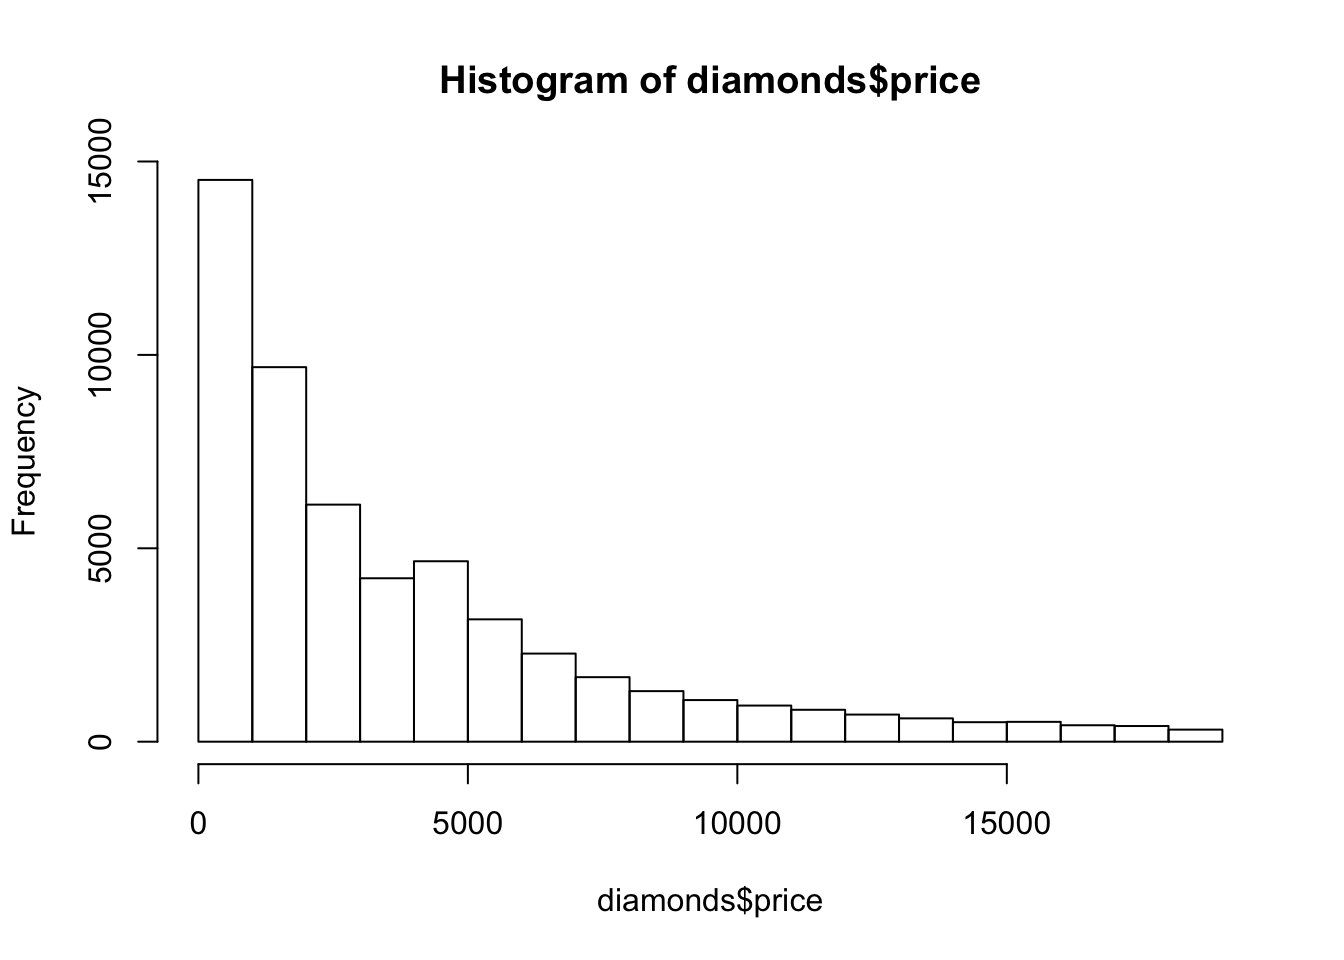
\includegraphics{_main_files/figure-latex/unnamed-chunk-48-1.png}

\begin{Shaded}
\begin{Highlighting}[]
\FunctionTok{boxplot}\NormalTok{(diamonds}\SpecialCharTok{$}\NormalTok{x)}
\end{Highlighting}
\end{Shaded}

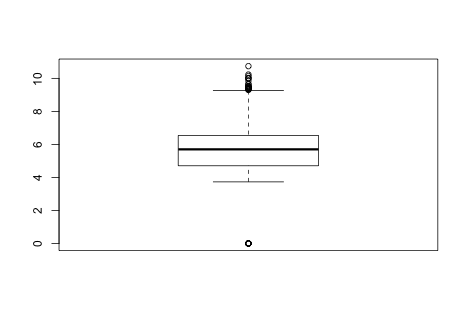
\includegraphics{_main_files/figure-latex/unnamed-chunk-49-1.png}

\hypertarget{visualisierung-mit-ggplot}{%
\subsection{\texorpdfstring{Visualisierung mit \texttt{ggplot()}}{Visualisierung mit ggplot()}}\label{visualisierung-mit-ggplot}}

Das Paket \texttt{ggplot2} ist Teil vom \texttt{tidyverse}. Hiermit lassen sich sehr flexible Graphiken gestalten. Wir werden ausschließlich mit diesem System arbeiten.

Die Syntax ist dabei auf den ersten Blick etwas komplexer.

Am Anfang steht der Befehl \texttt{ggplot(x)} mit dem Datensatz als Parameter

\begin{Shaded}
\begin{Highlighting}[]
\FunctionTok{ggplot}\NormalTok{(}\AttributeTok{data=}\NormalTok{diamonds)}
\end{Highlighting}
\end{Shaded}


\includegraphics{_main_files/figure-latex/unnamed-chunk-50-1.png}

Mit einem Mapping-Parameter legen wir die Dimensionen fest:

\begin{Shaded}
\begin{Highlighting}[]
\FunctionTok{ggplot}\NormalTok{(}\AttributeTok{data=}\NormalTok{diamonds, }\AttributeTok{mapping=}\FunctionTok{aes}\NormalTok{(}\AttributeTok{x=}\NormalTok{price, }\AttributeTok{y=}\NormalTok{carat))}
\end{Highlighting}
\end{Shaded}

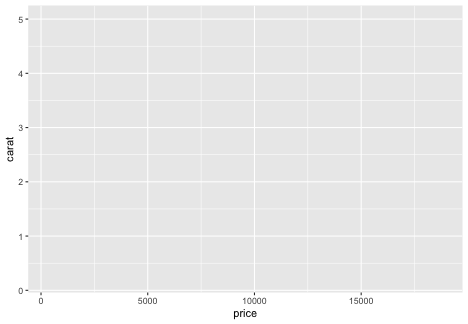
\includegraphics{_main_files/figure-latex/unnamed-chunk-51-1.png}

Das gleiche ohne Parameternamen:

\begin{Shaded}
\begin{Highlighting}[]
\FunctionTok{ggplot}\NormalTok{(diamonds, }\FunctionTok{aes}\NormalTok{(price, carat))}
\end{Highlighting}
\end{Shaded}

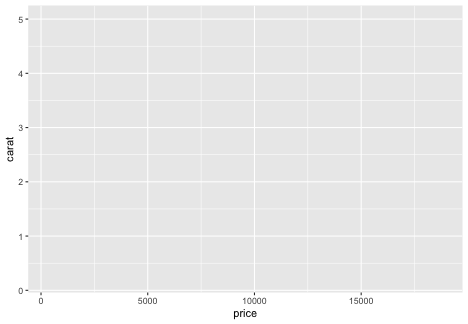
\includegraphics{_main_files/figure-latex/unnamed-chunk-52-1.png}

Nun kann mit dem \texttt{+}-Operator ein ``geometrischer'' Layer hinzugefügt werden:

\begin{Shaded}
\begin{Highlighting}[]
\FunctionTok{ggplot}\NormalTok{(diamonds, }\FunctionTok{aes}\NormalTok{(}\AttributeTok{x=}\NormalTok{carat, }\AttributeTok{y=}\NormalTok{price)) }\SpecialCharTok{+}
  \FunctionTok{geom\_point}\NormalTok{()}
\end{Highlighting}
\end{Shaded}

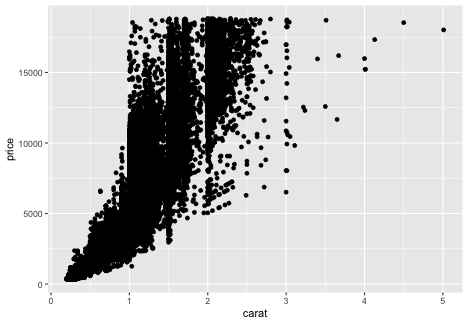
\includegraphics{_main_files/figure-latex/unnamed-chunk-53-1.png}

Weitere \texttt{geom}-Layer lassen sich mit dem \texttt{+}-Operator hinzufügen:

\begin{Shaded}
\begin{Highlighting}[]
\FunctionTok{ggplot}\NormalTok{(diamonds, }\FunctionTok{aes}\NormalTok{(}\AttributeTok{x=}\NormalTok{carat, }\AttributeTok{y=}\NormalTok{price)) }\SpecialCharTok{+}
  \FunctionTok{geom\_point}\NormalTok{() }\SpecialCharTok{+}
  \FunctionTok{geom\_smooth}\NormalTok{()}
\end{Highlighting}
\end{Shaded}

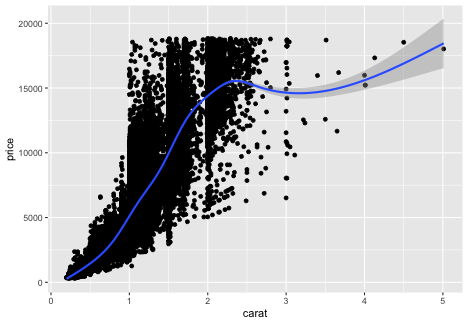
\includegraphics{_main_files/figure-latex/unnamed-chunk-54-1.png}

Die Layer-Funktionen können durch Parameter angepasst werden:

\begin{Shaded}
\begin{Highlighting}[]
\FunctionTok{ggplot}\NormalTok{(diamonds, }\FunctionTok{aes}\NormalTok{(}\AttributeTok{x=}\NormalTok{carat, }\AttributeTok{y=}\NormalTok{price)) }\SpecialCharTok{+}
  \FunctionTok{geom\_point}\NormalTok{(}\AttributeTok{size=}\FloatTok{0.5}\NormalTok{) }\SpecialCharTok{+}
  \FunctionTok{geom\_smooth}\NormalTok{(}\AttributeTok{color=}\StringTok{"red"}\NormalTok{)}
\end{Highlighting}
\end{Shaded}

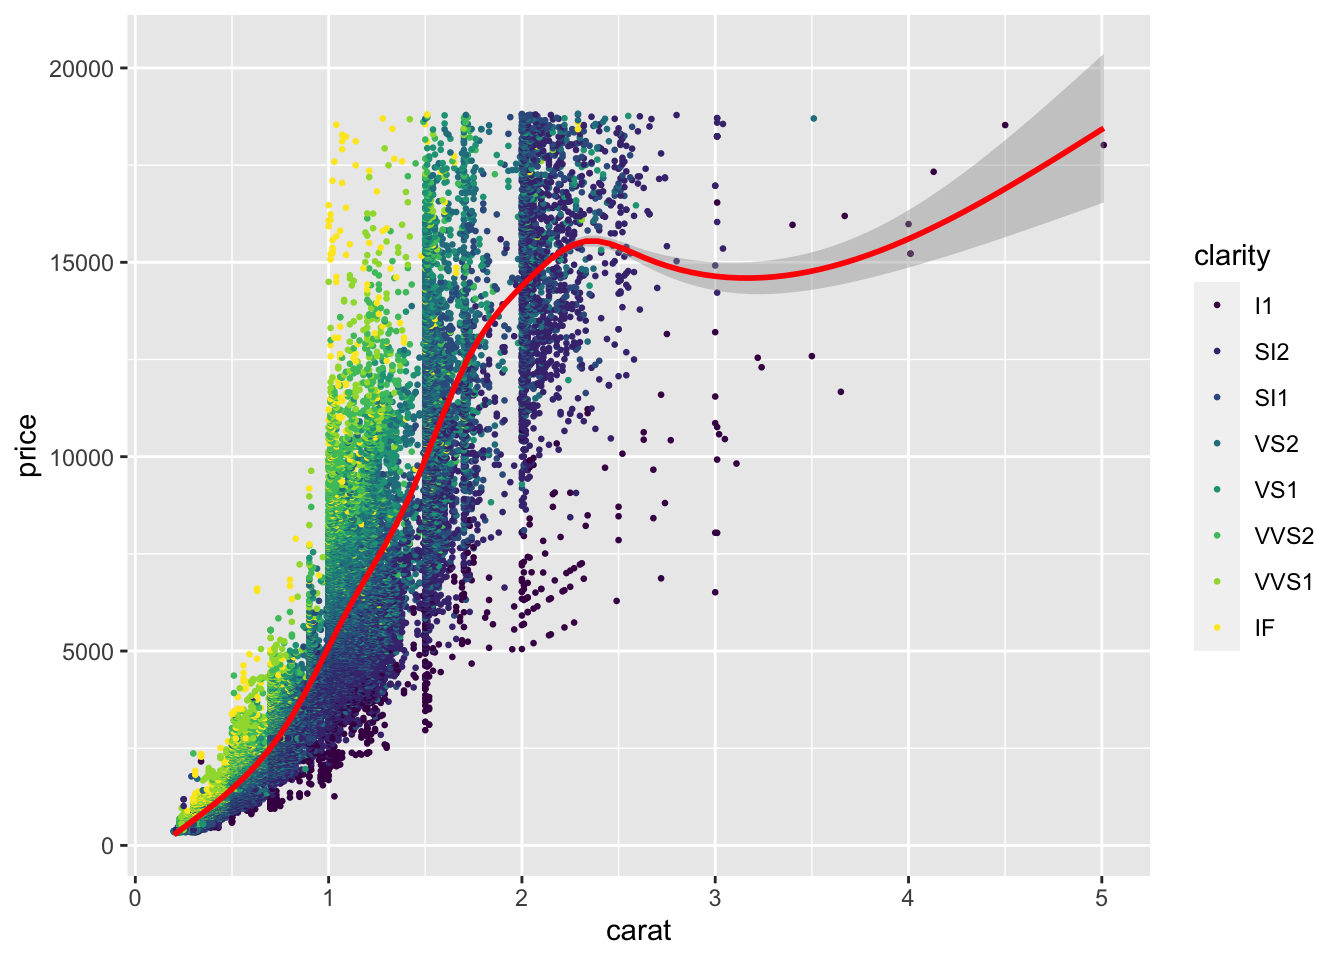
\includegraphics{_main_files/figure-latex/unnamed-chunk-55-1.png}

Dabei lassen sich in den einzelnen Layers mappings hinzufügen oder verändern:

\begin{Shaded}
\begin{Highlighting}[]
\FunctionTok{ggplot}\NormalTok{(diamonds, }\FunctionTok{aes}\NormalTok{(}\AttributeTok{x=}\NormalTok{carat, }\AttributeTok{y=}\NormalTok{price)) }\SpecialCharTok{+}
  \FunctionTok{geom\_point}\NormalTok{(}\FunctionTok{aes}\NormalTok{(}\AttributeTok{color=}\NormalTok{clarity), }\AttributeTok{size=}\FloatTok{0.5}\NormalTok{) }\SpecialCharTok{+}
  \FunctionTok{geom\_smooth}\NormalTok{(}\AttributeTok{color=}\StringTok{"red"}\NormalTok{)}
\end{Highlighting}
\end{Shaded}

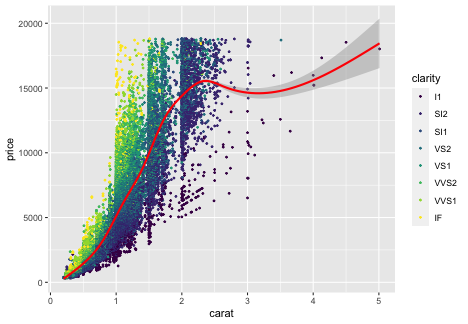
\includegraphics{_main_files/figure-latex/unnamed-chunk-56-1.png}

Schließlich lassen sich noch viele weitere optische Aspekte anpassen, z.B. Achsen, Farben, etc.:

\begin{Shaded}
\begin{Highlighting}[]
\FunctionTok{ggplot}\NormalTok{(diamonds, }\FunctionTok{aes}\NormalTok{(}\AttributeTok{x=}\NormalTok{carat, }\AttributeTok{y=}\NormalTok{price)) }\SpecialCharTok{+}
  \FunctionTok{geom\_point}\NormalTok{(}\FunctionTok{aes}\NormalTok{(}\AttributeTok{color=}\NormalTok{clarity), }\AttributeTok{size=}\FloatTok{0.5}\NormalTok{) }\SpecialCharTok{+}
  \FunctionTok{geom\_smooth}\NormalTok{(}\AttributeTok{color=}\StringTok{"red"}\NormalTok{) }\SpecialCharTok{+}
  \FunctionTok{scale\_x\_continuous}\NormalTok{(}\StringTok{"Karatzahl"}\NormalTok{, }\AttributeTok{breaks=}\FunctionTok{seq}\NormalTok{(}\DecValTok{0}\NormalTok{,}\DecValTok{5}\NormalTok{,}\FloatTok{0.5}\NormalTok{)) }\SpecialCharTok{+}
  \FunctionTok{scale\_y\_continuous}\NormalTok{(}\StringTok{"Preis"}\NormalTok{) }\SpecialCharTok{+}
  \FunctionTok{scale\_color\_brewer}\NormalTok{(}\StringTok{"Klarheit"}\NormalTok{) }\SpecialCharTok{+}
  \FunctionTok{theme\_dark}\NormalTok{()}
\end{Highlighting}
\end{Shaded}

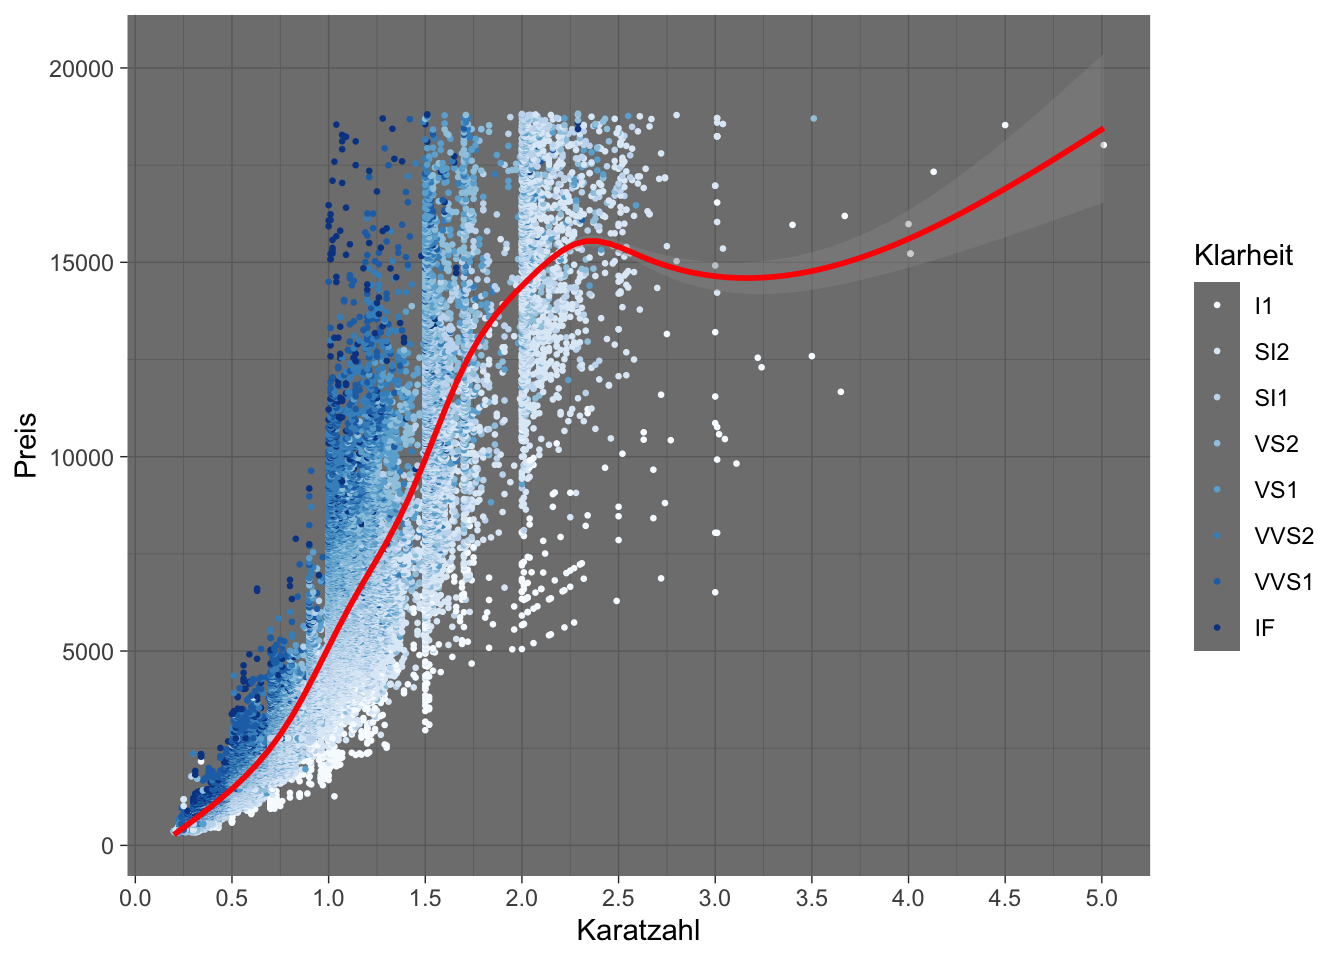
\includegraphics{_main_files/figure-latex/unnamed-chunk-57-1.png}

\hypertarget{aufgaben-2}{%
\subsection{Aufgaben}\label{aufgaben-2}}

Versuchen Sie, folgende Visualisierungen des Datensatzes \texttt{diamonds} auszugeben:

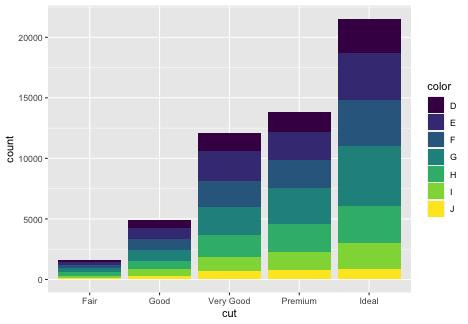
\includegraphics{_main_files/figure-latex/unnamed-chunk-58-1.png}

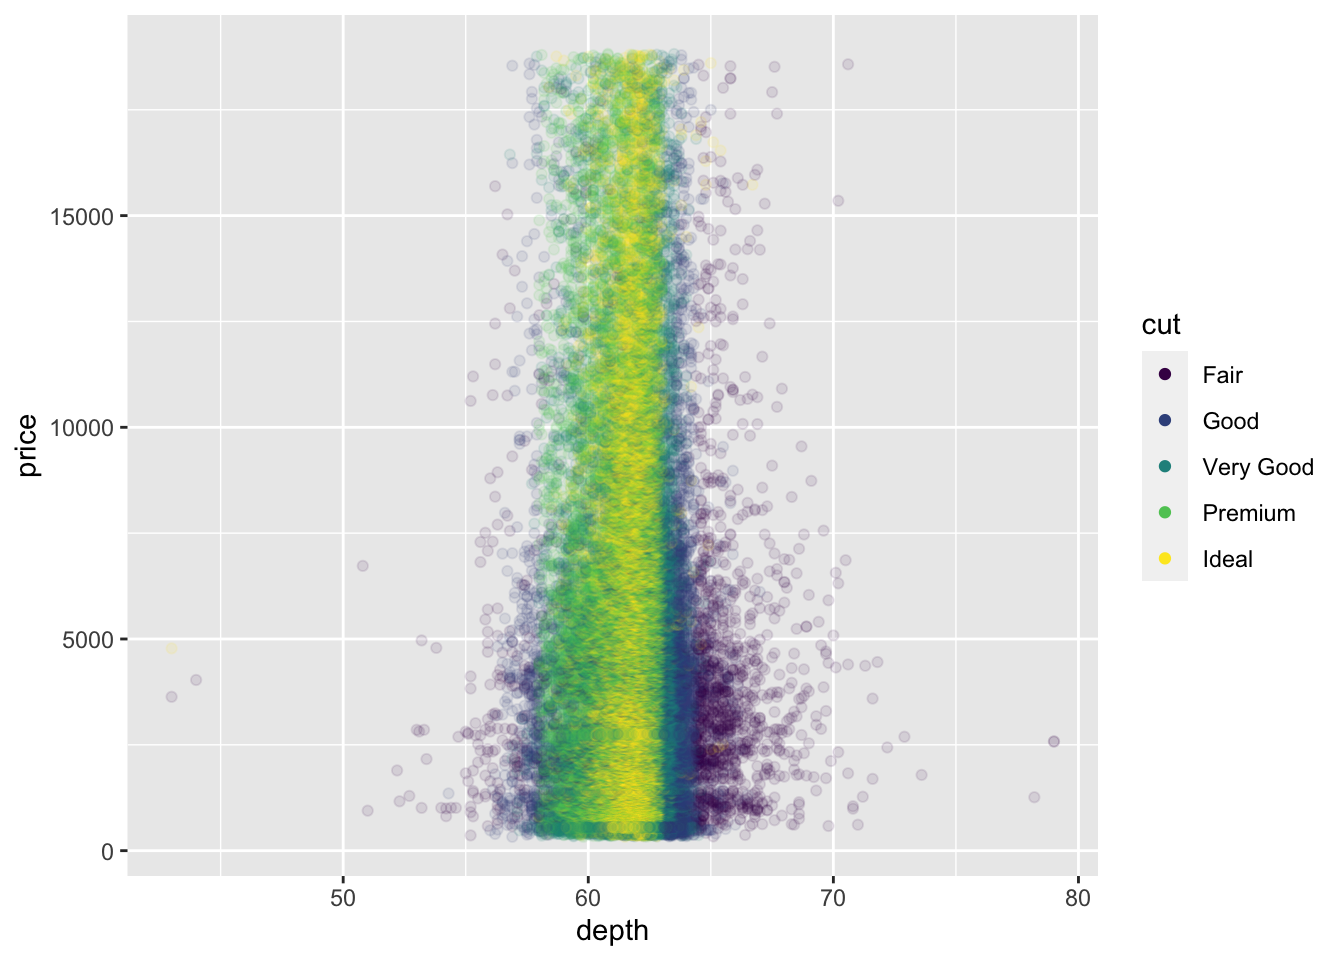
\includegraphics{_main_files/figure-latex/unnamed-chunk-59-1.png}

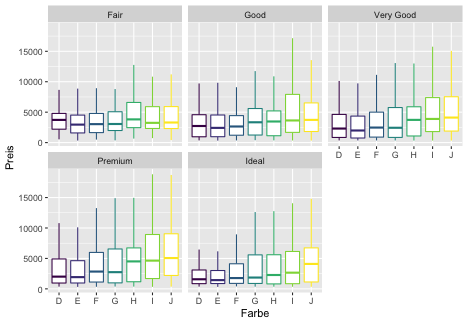
\includegraphics{_main_files/figure-latex/unnamed-chunk-60-1.png}

\hypertarget{r-for-data-science}{%
\subsubsection{R for Data Science}\label{r-for-data-science}}

Schauen Sie sich die Publikation \href{https://r4ds.had.co.nz/}{R for Data Science} an.

Was ist das für ein Buch? Wer ist das Zielpublikum?

Lesen Sie das Kapitel ``3: Data Visualization'' und vollziehen Sie die Visualisierungen nach.

Bearbeiten Sie die Aufgaben.

Bearbeiten Sie die \href{https://rstudio.cloud/learn/primers/3}{RStudio Primers zu Datenvisualisierung}.

\hypertarget{text-shelton-et-al.-2014}{%
\section{Text: Shelton et al.~2014}\label{text-shelton-et-al.-2014}}

\hypertarget{lesetext-1}{%
\subsection{Lesetext}\label{lesetext-1}}

Shelton, Taylor, Ate Poorthuis, Mark Graham und Matthew Zook. 2014. Mapping the Data Shadows of Hurricane Sandy. Uncovering the Sociospatial Dimensions of `Big Data'. \emph{Geoforum 52.} 167--79.

\hypertarget{fragen-an-den-text-1}{%
\subsection{Fragen an den Text}\label{fragen-an-den-text-1}}

\begin{enumerate}
\def\labelenumi{\arabic{enumi}.}
\tightlist
\item
  Um welche Art von Text handelt es sich? Wer sind die Autoren, und an wen wenden sie sich?
\item
  Was war Hurricane Sandy, von dem der Text erzählt? Warum wird ausgerechnet dieser Hurricane herangezogen?
\item
  Welche Methoden wenden die Autoren an, und zu welchen Ergebnissen kommen sie?
\item
  Im Abstract versprechen die Autoren: ``We also seek to fill a conceptual lacuna\ldots{}'' Was heißt das, und wie geht der Text das an?
\item
  In welchen Punkten finden Sie den Text überzeugend? Welche Kritik haben Sie am Text?
\end{enumerate}

\hypertarget{geodaten}{%
\section{Geodaten}\label{geodaten}}

\hypertarget{lernziele-dieser-sitzung-2}{%
\subsection{Lernziele dieser Sitzung}\label{lernziele-dieser-sitzung-2}}

Sie können\ldots{}

\begin{itemize}
\tightlist
\item
  Pipes benutzen
\item
  einfache \texttt{dplyr}-Befehle ausführen
\item
  Koordinaten visualisieren
\end{itemize}

\hypertarget{voraussetzungen-1}{%
\subsection{Voraussetzungen}\label{voraussetzungen-1}}

Wir laden erstmal \texttt{tidyverse}:

\begin{Shaded}
\begin{Highlighting}[]
\FunctionTok{library}\NormalTok{(tidyverse)}
\end{Highlighting}
\end{Shaded}

\hypertarget{exkurs-pipes}{%
\subsection{Exkurs: Pipes}\label{exkurs-pipes}}

Teil vom \texttt{tidyverse} ist auch das Paket \texttt{magrittr}, das einen besonderen Operator enthält: \texttt{\%\textgreater{}\%}

Der Operator \texttt{\%\textgreater{}\%} heißt ``Pipe'' und setzt das Ergebnis der vorherigen Funktion als ersten Parameter in die nächste Funktion ein. Zur Veranschaulichung:

\begin{Shaded}
\begin{Highlighting}[]
\NormalTok{anzahl\_buchstaben }\OtherTok{\textless{}{-}} \FunctionTok{length}\NormalTok{(letters)}
\FunctionTok{sqrt}\NormalTok{(anzahl\_buchstaben)}
\end{Highlighting}
\end{Shaded}

\ldots ist das gleiche wie\ldots{}

\begin{Shaded}
\begin{Highlighting}[]
\FunctionTok{sqrt}\NormalTok{(}\FunctionTok{length}\NormalTok{(letters))}
\end{Highlighting}
\end{Shaded}

\ldots ist das gleiche wie\ldots{}

\begin{Shaded}
\begin{Highlighting}[]
\FunctionTok{length}\NormalTok{(letters) }\SpecialCharTok{\%\textgreater{}\%}
  \FunctionTok{sqrt}\NormalTok{()}
\end{Highlighting}
\end{Shaded}

\ldots ist das gleiche wie\ldots{}

\begin{Shaded}
\begin{Highlighting}[]
\NormalTok{letters }\SpecialCharTok{\%\textgreater{}\%}
\NormalTok{  length }\SpecialCharTok{\%\textgreater{}\%}
  \FunctionTok{sqrt}\NormalTok{()}
\end{Highlighting}
\end{Shaded}

So können beliebig viele Funktionen aneinandergereiht werden. Und mit \texttt{-\textgreater{}} kann eine Variable „in die andere Richtung`` zugewiesen werden

\begin{Shaded}
\begin{Highlighting}[]
\NormalTok{letters }\SpecialCharTok{\%\textgreater{}\%}
  \FunctionTok{length}\NormalTok{() }\SpecialCharTok{\%\textgreater{}\%}
  \FunctionTok{sqrt}\NormalTok{() }\SpecialCharTok{\%\textgreater{}\%}
  \FunctionTok{round}\NormalTok{() }\SpecialCharTok{\%\textgreater{}\%}
  \FunctionTok{as.character}\NormalTok{() }\OtherTok{{-}\textgreater{}}
\NormalTok{  my\_var}
\end{Highlighting}
\end{Shaded}

Gerade bei komplizierteren Zusammenhängen wird der Code so oft lesbarer, weil die Logik von links nach rechts, bzw. von oben nach unten gelesen werden kann.

\hypertarget{daten-importieren}{%
\subsection{Daten importieren}\label{daten-importieren}}

Beim Open-Data-Portal der Stadt Frankfurt steht ein \href{http://offenedaten.frankfurt.de/dataset/baumkataster-frankfurt-am-main}{Baumkataster} zur Verfügung.

Die Datei im CSV-Format (comma separated values) kann entweder heruntergeladen und durch klicken importiert werden, oder direkt über den Befehl:

\begin{Shaded}
\begin{Highlighting}[]
\NormalTok{baumkataster }\OtherTok{\textless{}{-}} \FunctionTok{read\_csv2}\NormalTok{(}\StringTok{"http://offenedaten.frankfurt.de/dataset/73c5a6b3{-}c033{-}4dad{-}bb7d{-}8783427dd233/resource/7a73520b{-}961a{-}4aad{-}a582{-}449e676c247c/download/gprojekteopen{-}datadatenamt{-}67datenbaumauswahl\_veroffentlichung\_4baumauswahl\_veroffentlichung\_4.csv"}\NormalTok{)}
\end{Highlighting}
\end{Shaded}

\hypertarget{uxfcberblick-verschaffen}{%
\subsection{Überblick verschaffen}\label{uxfcberblick-verschaffen}}

Mit \texttt{summary()} lässt sich eine Zusammenfassung der Werte generieren:

\begin{Shaded}
\begin{Highlighting}[]
\FunctionTok{summary}\NormalTok{(baumkataster)}
\DocumentationTok{\#\#  Gattung/Art/Deutscher Name   Baumnummer     }
\DocumentationTok{\#\#  Length:118403              Min.   :    1.0  }
\DocumentationTok{\#\#  Class :character           1st Qu.:   24.0  }
\DocumentationTok{\#\#  Mode  :character           Median :   82.0  }
\DocumentationTok{\#\#                             Mean   :  232.7  }
\DocumentationTok{\#\#                             3rd Qu.:  270.0  }
\DocumentationTok{\#\#                             Max.   :20158.0  }
\DocumentationTok{\#\#                             NA\textquotesingle{}s   :1853     }
\DocumentationTok{\#\#     Objekt            Pflanzjahr   Kronendurchmesser}
\DocumentationTok{\#\#  Length:118403      Min.   :1645   Min.   : 2.000   }
\DocumentationTok{\#\#  Class :character   1st Qu.:1970   1st Qu.: 4.000   }
\DocumentationTok{\#\#  Mode  :character   Median :1982   Median : 6.000   }
\DocumentationTok{\#\#                     Mean   :1979   Mean   : 6.688   }
\DocumentationTok{\#\#                     3rd Qu.:1995   3rd Qu.: 9.000   }
\DocumentationTok{\#\#                     Max.   :2017   Max.   :63.000   }
\DocumentationTok{\#\#                                                     }
\DocumentationTok{\#\#     HOCHWERT         RECHTSWERT    }
\DocumentationTok{\#\#  Min.   :5545117   Min.   :463163  }
\DocumentationTok{\#\#  1st Qu.:5550428   1st Qu.:472715  }
\DocumentationTok{\#\#  Median :5552601   Median :475219  }
\DocumentationTok{\#\#  Mean   :5552953   Mean   :475244  }
\DocumentationTok{\#\#  3rd Qu.:5555165   3rd Qu.:478201  }
\DocumentationTok{\#\#  Max.   :5563639   Max.   :485361  }
\DocumentationTok{\#\# }
\end{Highlighting}
\end{Shaded}

Genauere Infos über diese Merkmale gibt es auf dem Datenportal.

\hypertarget{visualisieren}{%
\subsection{Visualisieren}\label{visualisieren}}

Wie in der letzten Lektion besprochen, lässt sich der Datensatz mit \texttt{ggplot()} visualisieren, z.B.:

\begin{Shaded}
\begin{Highlighting}[]
\FunctionTok{ggplot}\NormalTok{(baumkataster, }\FunctionTok{aes}\NormalTok{(}\AttributeTok{x=}\NormalTok{Kronendurchmesser)) }\SpecialCharTok{+}
  \FunctionTok{geom\_histogram}\NormalTok{()}
\end{Highlighting}
\end{Shaded}

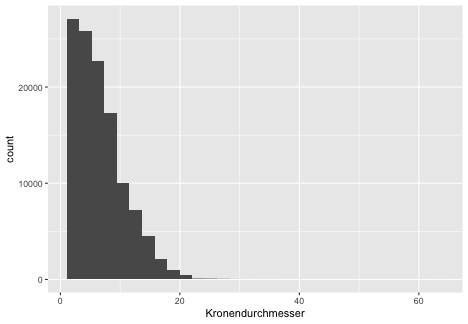
\includegraphics{_main_files/figure-latex/unnamed-chunk-69-1.png}

Eine neue Messreihe lässt sich z.B. so errechnen:

\begin{Shaded}
\begin{Highlighting}[]
\NormalTok{alter }\OtherTok{\textless{}{-}} \DecValTok{2020} \SpecialCharTok{{-}}\NormalTok{ baumkataster}\SpecialCharTok{$}\NormalTok{Pflanzjahr}
\FunctionTok{head}\NormalTok{(alter)}
\DocumentationTok{\#\# [1] 100 100 100 100 100 100}
\end{Highlighting}
\end{Shaded}

Der Befehl \texttt{mutate()} funktioniert sehr ähnlich, gibt aber den veränderten Datensatz zurück:

\begin{Shaded}
\begin{Highlighting}[]
\FunctionTok{mutate}\NormalTok{(baumkataster, }\AttributeTok{alter =} \DecValTok{2020} \SpecialCharTok{{-}}\NormalTok{ Pflanzjahr)}
\DocumentationTok{\#\# \# A tibble: 118,403 x 8}
\DocumentationTok{\#\#    \textasciigrave{}Gattung/Art/De\textasciitilde{} Baumnummer Objekt Pflanzjahr}
\DocumentationTok{\#\#    \textless{}chr\textgreater{}                 \textless{}dbl\textgreater{} \textless{}chr\textgreater{}       \textless{}dbl\textgreater{}}
\DocumentationTok{\#\#  1 Platanus x hisp\textasciitilde{}          1 Acker\textasciitilde{}       1920}
\DocumentationTok{\#\#  2 Platanus x hisp\textasciitilde{}          2 Acker\textasciitilde{}       1920}
\DocumentationTok{\#\#  3 Platanus x hisp\textasciitilde{}          3 Acker\textasciitilde{}       1920}
\DocumentationTok{\#\#  4 Platanus x hisp\textasciitilde{}          4 Acker\textasciitilde{}       1920}
\DocumentationTok{\#\#  5 Platanus x hisp\textasciitilde{}          5 Acker\textasciitilde{}       1920}
\DocumentationTok{\#\#  6 Platanus x hisp\textasciitilde{}          6 Acker\textasciitilde{}       1920}
\DocumentationTok{\#\#  7 Platanus x hisp\textasciitilde{}          7 Acker\textasciitilde{}       1920}
\DocumentationTok{\#\#  8 Platanus x hisp\textasciitilde{}          8 Acker\textasciitilde{}       1920}
\DocumentationTok{\#\#  9 Platanus x hisp\textasciitilde{}          9 Acker\textasciitilde{}       1920}
\DocumentationTok{\#\# 10 Platanus x hisp\textasciitilde{}         10 Acker\textasciitilde{}       1920}
\DocumentationTok{\#\# \# ... with 118,393 more rows, and 4 more variables:}
\DocumentationTok{\#\# \#   Kronendurchmesser \textless{}dbl\textgreater{}, HOCHWERT \textless{}dbl\textgreater{},}
\DocumentationTok{\#\# \#   RECHTSWERT \textless{}dbl\textgreater{}, alter \textless{}dbl\textgreater{}}
\end{Highlighting}
\end{Shaded}

Derselbe Befehl mit dem Pipe-Operator:

\begin{Shaded}
\begin{Highlighting}[]
\NormalTok{baumkataster }\SpecialCharTok{\%\textgreater{}\%}
  \FunctionTok{mutate}\NormalTok{(}\AttributeTok{alter =} \DecValTok{2020} \SpecialCharTok{{-}}\NormalTok{ Pflanzjahr)}
\DocumentationTok{\#\# \# A tibble: 118,403 x 8}
\DocumentationTok{\#\#    \textasciigrave{}Gattung/Art/De\textasciitilde{} Baumnummer Objekt Pflanzjahr}
\DocumentationTok{\#\#    \textless{}chr\textgreater{}                 \textless{}dbl\textgreater{} \textless{}chr\textgreater{}       \textless{}dbl\textgreater{}}
\DocumentationTok{\#\#  1 Platanus x hisp\textasciitilde{}          1 Acker\textasciitilde{}       1920}
\DocumentationTok{\#\#  2 Platanus x hisp\textasciitilde{}          2 Acker\textasciitilde{}       1920}
\DocumentationTok{\#\#  3 Platanus x hisp\textasciitilde{}          3 Acker\textasciitilde{}       1920}
\DocumentationTok{\#\#  4 Platanus x hisp\textasciitilde{}          4 Acker\textasciitilde{}       1920}
\DocumentationTok{\#\#  5 Platanus x hisp\textasciitilde{}          5 Acker\textasciitilde{}       1920}
\DocumentationTok{\#\#  6 Platanus x hisp\textasciitilde{}          6 Acker\textasciitilde{}       1920}
\DocumentationTok{\#\#  7 Platanus x hisp\textasciitilde{}          7 Acker\textasciitilde{}       1920}
\DocumentationTok{\#\#  8 Platanus x hisp\textasciitilde{}          8 Acker\textasciitilde{}       1920}
\DocumentationTok{\#\#  9 Platanus x hisp\textasciitilde{}          9 Acker\textasciitilde{}       1920}
\DocumentationTok{\#\# 10 Platanus x hisp\textasciitilde{}         10 Acker\textasciitilde{}       1920}
\DocumentationTok{\#\# \# ... with 118,393 more rows, and 4 more variables:}
\DocumentationTok{\#\# \#   Kronendurchmesser \textless{}dbl\textgreater{}, HOCHWERT \textless{}dbl\textgreater{},}
\DocumentationTok{\#\# \#   RECHTSWERT \textless{}dbl\textgreater{}, alter \textless{}dbl\textgreater{}}
\end{Highlighting}
\end{Shaded}

So lassen sich auch hier verschiedene Befehle verknüpfen. \texttt{filter()} beschränkt den Datensatz auf Merkmalsträger, die den Kriterien entsprechen:

\begin{Shaded}
\begin{Highlighting}[]
\NormalTok{baumkataster }\SpecialCharTok{\%\textgreater{}\%}
  \FunctionTok{mutate}\NormalTok{(}\AttributeTok{alter =} \DecValTok{2020} \SpecialCharTok{{-}}\NormalTok{ Pflanzjahr) }\SpecialCharTok{\%\textgreater{}\%}
  \FunctionTok{filter}\NormalTok{(alter }\SpecialCharTok{\textgreater{}} \DecValTok{30}\NormalTok{) }\OtherTok{{-}\textgreater{}}
\NormalTok{  alte\_baeume}

\FunctionTok{summary}\NormalTok{(alte\_baeume)}
\DocumentationTok{\#\#  Gattung/Art/Deutscher Name   Baumnummer     }
\DocumentationTok{\#\#  Length:73859               Min.   :    1.0  }
\DocumentationTok{\#\#  Class :character           1st Qu.:   29.0  }
\DocumentationTok{\#\#  Mode  :character           Median :   97.0  }
\DocumentationTok{\#\#                             Mean   :  263.2  }
\DocumentationTok{\#\#                             3rd Qu.:  314.0  }
\DocumentationTok{\#\#                             Max.   :10489.0  }
\DocumentationTok{\#\#                             NA\textquotesingle{}s   :684      }
\DocumentationTok{\#\#     Objekt            Pflanzjahr   Kronendurchmesser}
\DocumentationTok{\#\#  Length:73859       Min.   :1645   Min.   : 2.000   }
\DocumentationTok{\#\#  Class :character   1st Qu.:1960   1st Qu.: 6.000   }
\DocumentationTok{\#\#  Mode  :character   Median :1974   Median : 8.000   }
\DocumentationTok{\#\#                     Mean   :1966   Mean   : 8.503   }
\DocumentationTok{\#\#                     3rd Qu.:1980   3rd Qu.:10.000   }
\DocumentationTok{\#\#                     Max.   :1989   Max.   :35.000   }
\DocumentationTok{\#\#                                                     }
\DocumentationTok{\#\#     HOCHWERT         RECHTSWERT         alter       }
\DocumentationTok{\#\#  Min.   :5545117   Min.   :463163   Min.   : 31.00  }
\DocumentationTok{\#\#  1st Qu.:5550415   1st Qu.:472667   1st Qu.: 40.00  }
\DocumentationTok{\#\#  Median :5552480   Median :475708   Median : 46.00  }
\DocumentationTok{\#\#  Mean   :5552593   Mean   :475402   Mean   : 53.54  }
\DocumentationTok{\#\#  3rd Qu.:5554589   3rd Qu.:478539   3rd Qu.: 60.00  }
\DocumentationTok{\#\#  Max.   :5563639   Max.   :485360   Max.   :375.00  }
\DocumentationTok{\#\# }
\end{Highlighting}
\end{Shaded}

Schließlich ergibt das Streudiagramm von Koordinaten so eine art Karte:

\begin{Shaded}
\begin{Highlighting}[]
\FunctionTok{ggplot}\NormalTok{(alte\_baeume) }\SpecialCharTok{+}
    \FunctionTok{geom\_point}\NormalTok{(}\AttributeTok{size =} \FloatTok{0.1}\NormalTok{, }\FunctionTok{aes}\NormalTok{(}\AttributeTok{x =}\NormalTok{ RECHTSWERT, }\AttributeTok{y =}\NormalTok{ HOCHWERT))}
\end{Highlighting}
\end{Shaded}

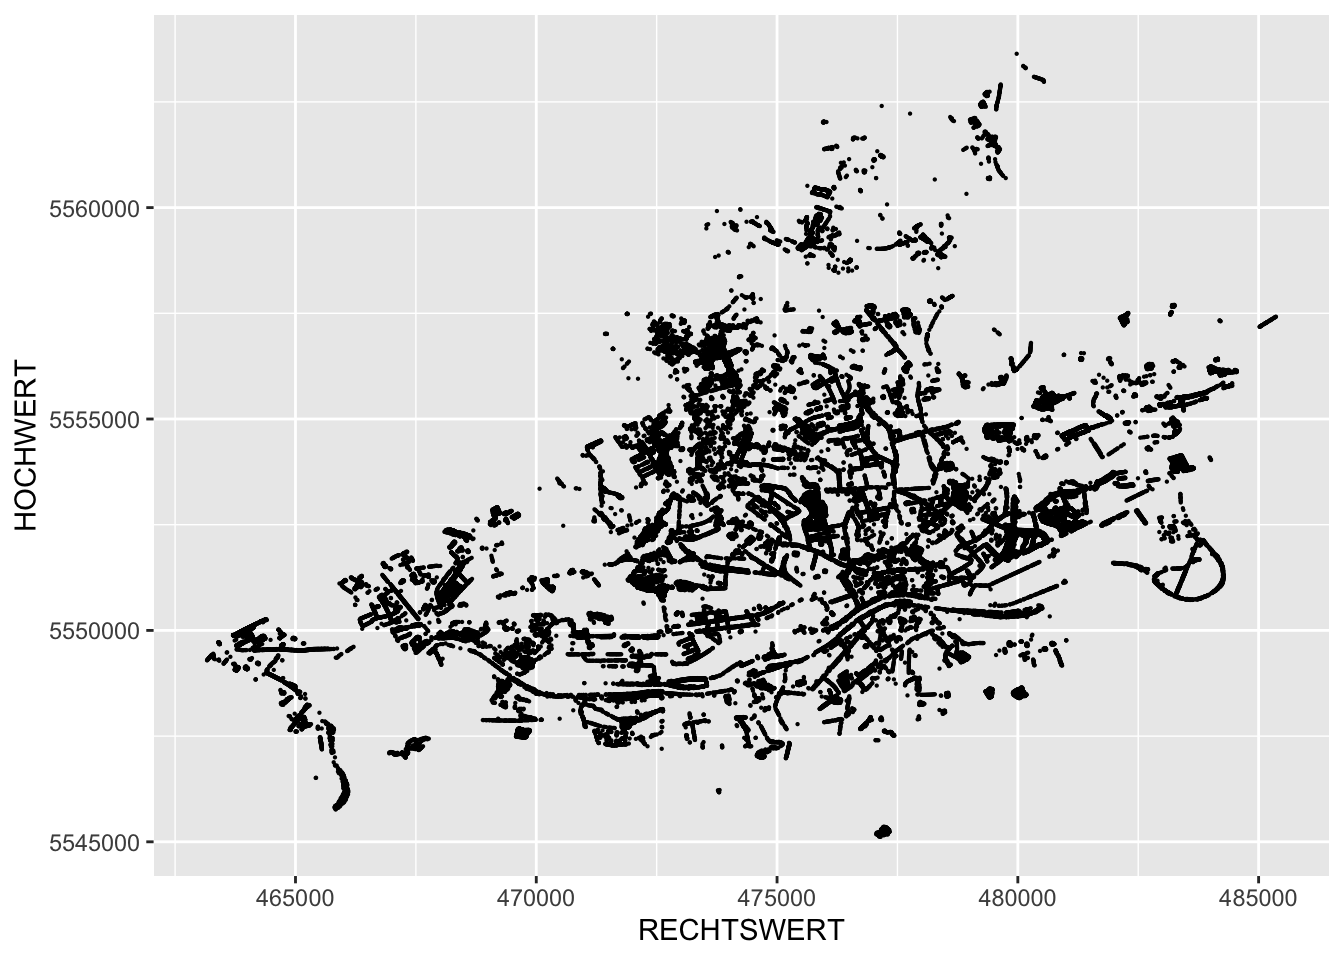
\includegraphics{_main_files/figure-latex/unnamed-chunk-74-1.png}

Diesen Ansatz werden wir in der nächsten Lektion vertiefen.

\hypertarget{aufgaben-3}{%
\subsection{Aufgaben}\label{aufgaben-3}}

\begin{enumerate}
\def\labelenumi{\arabic{enumi}.}
\item
  Besuchen Sie \url{https://pleiades.stoa.org/} - worum geht es hier?
\item
  Finden Sie den kompletten aktuellen Datensatz für „locations`` als CSV-Datei.
\item
  Importieren Sie ihn in R und weisen Sie dem Datensatz den Namen \texttt{pleiades} zu.
\item
  Finden Sie geeignete Werte für (einzelne) Längen- und Breitengrade im Datensatz.
\item
  Plotten Sie die Koordinaten auf x- und y-Achse mit \texttt{ggplot()}. Was erkennen Sie?
\item
  Halbieren Sie die Größe und setzen Sie den Alpha-Wert der Punkte auf 0,2.
\item
  Bringen Sie die Grafik in die Mercator-Projektion.
\item
  Schauen Sie sich diesen Befehl an:
\end{enumerate}

\begin{Shaded}
\begin{Highlighting}[]
\FunctionTok{map\_data}\NormalTok{(}\StringTok{"world"}\NormalTok{) }\SpecialCharTok{\%\textgreater{}\%}
  \FunctionTok{ggplot}\NormalTok{() }\SpecialCharTok{+}
    \FunctionTok{geom\_polygon}\NormalTok{(}\AttributeTok{mapping =} \FunctionTok{aes}\NormalTok{(}\AttributeTok{x =}\NormalTok{ long,}
                               \AttributeTok{y =}\NormalTok{ lat,}
                               \AttributeTok{group =}\NormalTok{ group)) }\SpecialCharTok{+}
    \FunctionTok{coord\_quickmap}\NormalTok{(}\AttributeTok{xlim =} \FunctionTok{c}\NormalTok{(}\SpecialCharTok{{-}}\DecValTok{8}\NormalTok{, }\DecValTok{40}\NormalTok{),}
                   \AttributeTok{ylim =} \FunctionTok{c}\NormalTok{(}\DecValTok{26}\NormalTok{, }\DecValTok{48}\NormalTok{))}
\end{Highlighting}
\end{Shaded}

\begin{enumerate}
\def\labelenumi{\arabic{enumi}.}
\setcounter{enumi}{8}
\item
  Versuchen Sie, jede einzelne Zeile nachzuvollziehen, indem Sie die entsprechenden Funktionen recherchieren.
\item
  Führen Sie den Befehl aus.
\item
  Ändern Sie die Farbe der Flächen in hellgrau.
\item
  Wählen Sie einen Kartenausschnitt, auf dem Portugal, Ägypten, Irak und Frankreich komplett zu sehen sind.
\item
  Plotten Sie auf diesem Hintergrund den Datensatz \texttt{pleiades}. Passen Sie dabei die Parameter so an, dass es Ihnen optisch zusagt.
\item
  Wählen Sie für die Karte die \href{https://de.wikipedia.org/wiki/Bonnesche_Projektion}{Bonnesche Projektion} mit Standardparallele bei 40°N.
\item
  Entfernen Sie alle Achsenbeschriftungen.
\item
  (Achtung: extrem knifflig!) Bilden Sie diese Grafik nach, die die Orte geordnet nach ältestem Fund darstellt:
\end{enumerate}

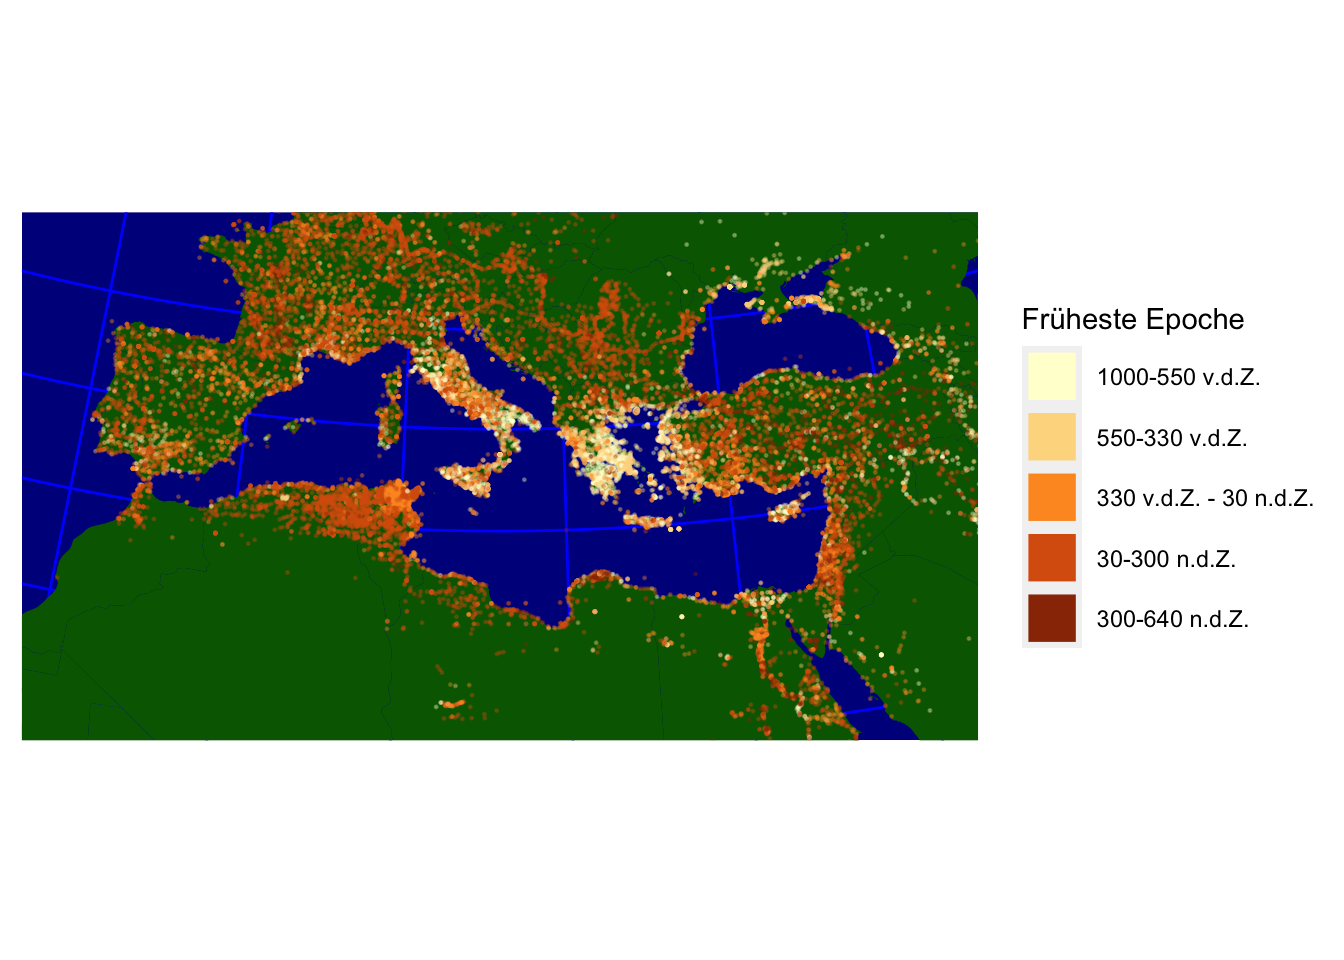
\includegraphics{_main_files/figure-latex/unnamed-chunk-87-1.png}

\hypertarget{choroplethen}{%
\section{Choroplethen}\label{choroplethen}}

\hypertarget{lernziele}{%
\subsection{Lernziele}\label{lernziele}}

Sie können\ldots{}

\begin{itemize}
\tightlist
\item
  Geodaten als Simple Features importieren,
\item
  CRS bestimmen und umwandeln,
\item
  einfache Verschneidungen von Simple Features durchführen und
\item
  Simple Features kartographisch darstellen.
\end{itemize}

\hypertarget{vorbereitung-1}{%
\subsection{Vorbereitung}\label{vorbereitung-1}}

Für diese Lektion werden zwei Pakete geladen:

\begin{Shaded}
\begin{Highlighting}[]
\FunctionTok{library}\NormalTok{(tidyverse)}
\FunctionTok{library}\NormalTok{(sf)}
\end{Highlighting}
\end{Shaded}

\hypertarget{ziel}{%
\subsection{Ziel}\label{ziel}}

Ziel ist, eine \href{https://de.wikipedia.org/wiki/Choroplethenkarte}{Choroplethenkarte} von Frankfurt zu erstellen, die die Versorgung mit Kiosken darstellt.

\hypertarget{grundkarte}{%
\subsection{Grundkarte}\label{grundkarte}}

Eine Shapefile der Frankfurter Stadtteile findet sich hier: \url{http://www.offenedaten.frankfurt.de/dataset/frankfurter-stadtteilgrenzen-fur-gis-systeme}

Wir laden die Zip-Datei herunter und speichern den enthaltenen Ordner \texttt{stadtteile} in unserem Arbeitsverzeichnis. Es ist eine gute Angewohnheit, einen Unterordner für Ressourcen anzulegen.

Dann importieren wir den Geodatensatz als Simple Features (Paket \texttt{sf}):

\begin{Shaded}
\begin{Highlighting}[]
\NormalTok{stadtteile }\OtherTok{\textless{}{-}} \FunctionTok{st\_read}\NormalTok{(}\StringTok{"resources/stadtteile/Stadtteile\_Frankfurt\_am\_Main.shp"}\NormalTok{)}
\DocumentationTok{\#\# Reading layer \textasciigrave{}Stadtteile\_Frankfurt\_am\_Main\textquotesingle{} from data source \textasciigrave{}/Users/till/teaching/2020x21\_Data\_Science/public/resources/stadtteile/Stadtteile\_Frankfurt\_am\_Main.shp\textquotesingle{} using driver \textasciigrave{}ESRI Shapefile\textquotesingle{}}
\DocumentationTok{\#\# Simple feature collection with 46 features and 2 fields}
\DocumentationTok{\#\# geometry type:  POLYGON}
\DocumentationTok{\#\# dimension:      XY}
\DocumentationTok{\#\# bbox:           xmin: 462292.7 ymin: 5540412 xmax: 485744.8 ymax: 5563925}
\DocumentationTok{\#\# projected CRS:  ETRS89 / UTM zone 32N}
\end{Highlighting}
\end{Shaded}

Simple Features sind Datensätze, die eine Spalte \texttt{geometry} enthalten, in der Geodaten in einem standardisierten Format hinterlegt sind.

\begin{Shaded}
\begin{Highlighting}[]
\FunctionTok{str}\NormalTok{(stadtteile)}
\DocumentationTok{\#\# Classes \textquotesingle{}sf\textquotesingle{} and \textquotesingle{}data.frame\textquotesingle{}:   46 obs. of  3 variables:}
\DocumentationTok{\#\#  $ STTLNR  : num  1 2 3 4 5 6 7 8 9 10 ...}
\DocumentationTok{\#\#  $ STTLNAME: Factor w/ 46 levels "Altstadt","Bahnhofsviertel",..: 1 22 2 45 44 30 29 32 7 17 ...}
\DocumentationTok{\#\#  $ geometry:sfc\_POLYGON of length 46; first list element: List of 1}
\DocumentationTok{\#\#   ..$ : num [1:46, 1:2] 476934 476890 476852 476813 476799 ...}
\DocumentationTok{\#\#   ..{-} attr(*, "class")= chr  "XY" "POLYGON" "sfg"}
\DocumentationTok{\#\#  {-} attr(*, "sf\_column")= chr "geometry"}
\DocumentationTok{\#\#  {-} attr(*, "agr")= Factor w/ 3 levels "constant","aggregate",..: NA NA}
\DocumentationTok{\#\#   ..{-} attr(*, "names")= chr  "STTLNR" "STTLNAME"}
\end{Highlighting}
\end{Shaded}

Eine Vorschau:

\begin{Shaded}
\begin{Highlighting}[]
\FunctionTok{ggplot}\NormalTok{(stadtteile) }\SpecialCharTok{+}
  \FunctionTok{geom\_sf}\NormalTok{() }\SpecialCharTok{+}
  \FunctionTok{geom\_sf\_label}\NormalTok{(}\FunctionTok{aes}\NormalTok{(}\AttributeTok{label =}\NormalTok{ STTLNAME), }\AttributeTok{size =} \DecValTok{2}\NormalTok{)}
\end{Highlighting}
\end{Shaded}

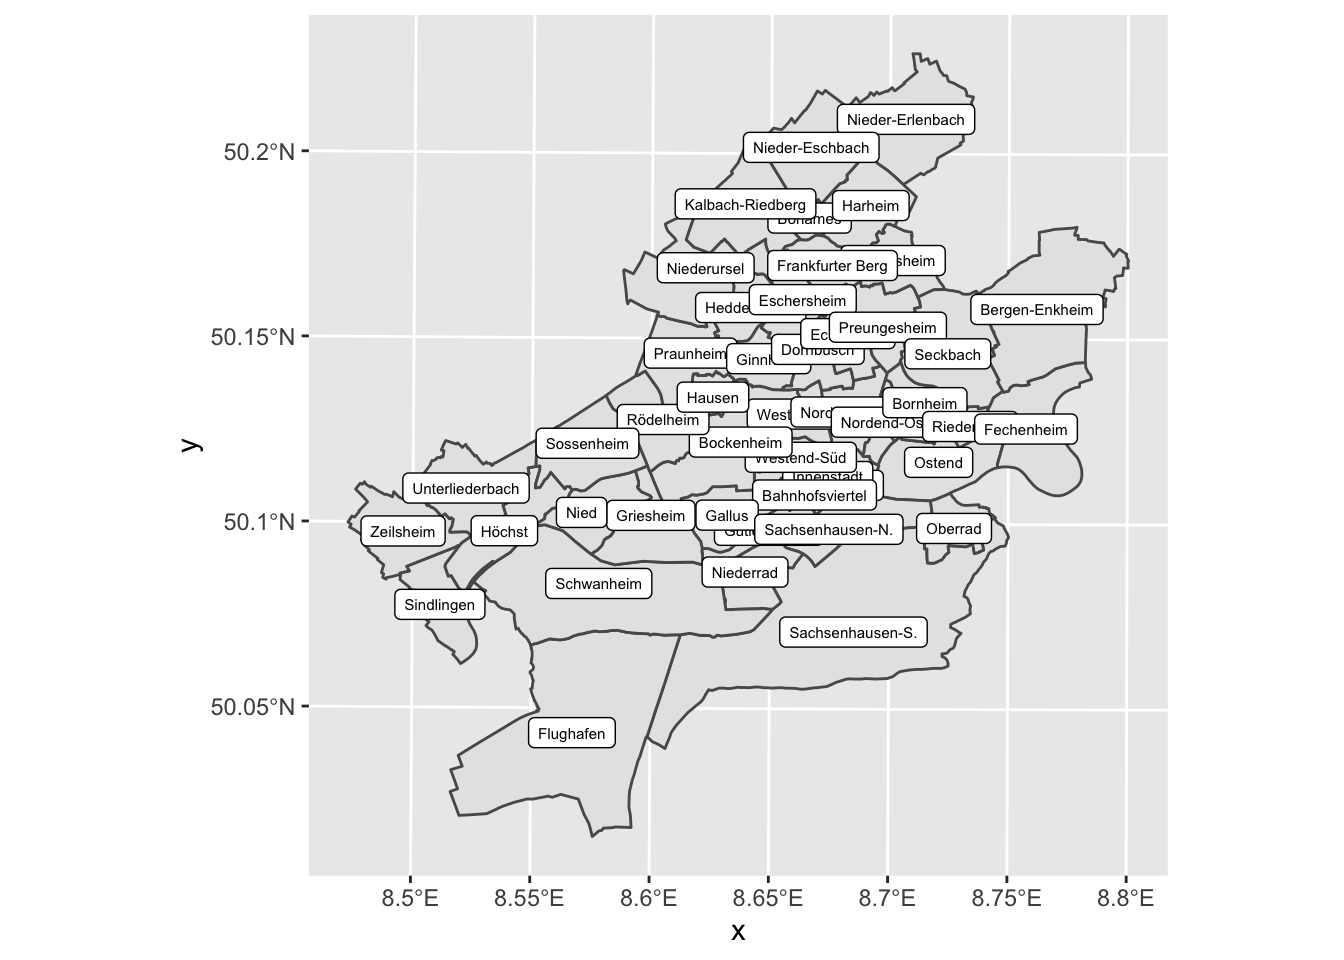
\includegraphics{_main_files/figure-latex/unnamed-chunk-91-1.png}

\hypertarget{osm-daten}{%
\subsection{OSM-Daten}\label{osm-daten}}

Im \href{https://wiki.openstreetmap.org/wiki/Map_Features}{OSM Wiki} suchen wir den richtigen \emph{tag} heraus. In diesem Fall \texttt{shop=kiosk}

Dann bauen wir auf \href{https://overpass-turbo.eu/}{Overpass Turbo} die Abfrage und laden den Datensatz herunter.

Schließlich importieren wir:

\begin{Shaded}
\begin{Highlighting}[]
\NormalTok{kioske }\OtherTok{\textless{}{-}} \FunctionTok{st\_read}\NormalTok{(}\StringTok{"resources/kioske.geojson"}\NormalTok{)}
\DocumentationTok{\#\# Reading layer \textasciigrave{}kioske\textquotesingle{} from data source \textasciigrave{}/Users/till/teaching/2020x21\_Data\_Science/public/resources/kioske.geojson\textquotesingle{} using driver \textasciigrave{}GeoJSON\textquotesingle{}}
\DocumentationTok{\#\# Simple feature collection with 325 features and 74 fields}
\DocumentationTok{\#\# geometry type:  GEOMETRY}
\DocumentationTok{\#\# dimension:      XY}
\DocumentationTok{\#\# bbox:           xmin: 8.505468 ymin: 50.04801 xmax: 8.789538 ymax: 50.20185}
\DocumentationTok{\#\# geographic CRS: WGS 84}
\end{Highlighting}
\end{Shaded}

Eine Vorschau:

\begin{Shaded}
\begin{Highlighting}[]
\FunctionTok{ggplot}\NormalTok{() }\SpecialCharTok{+}
  \FunctionTok{geom\_sf}\NormalTok{(}\AttributeTok{data =}\NormalTok{ stadtteile) }\SpecialCharTok{+}
  \FunctionTok{geom\_sf}\NormalTok{(}\AttributeTok{data =}\NormalTok{ kioske)}
\end{Highlighting}
\end{Shaded}

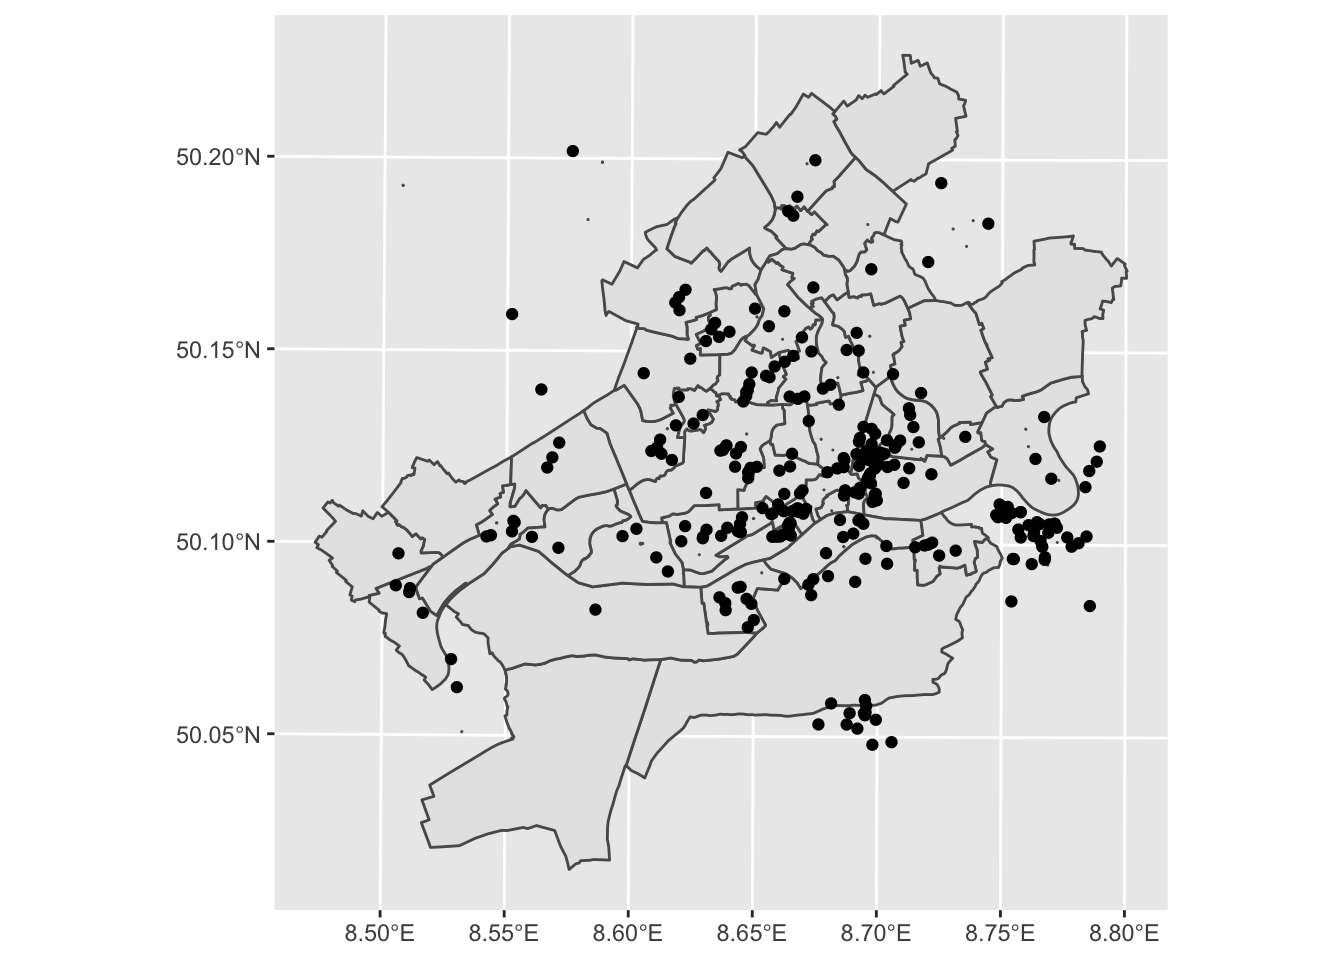
\includegraphics{_main_files/figure-latex/unnamed-chunk-93-1.png}

\hypertarget{koordinatenreferenzsysteme}{%
\subsection{Koordinatenreferenzsysteme}\label{koordinatenreferenzsysteme}}

Der OSM-Datensatz ist mit WGS84 (EPSG 4326) referenziert:

\begin{Shaded}
\begin{Highlighting}[]
\FunctionTok{st\_crs}\NormalTok{(kioske)}
\DocumentationTok{\#\# Coordinate Reference System:}
\DocumentationTok{\#\#   User input: WGS 84 }
\DocumentationTok{\#\#   wkt:}
\DocumentationTok{\#\# GEOGCRS["WGS 84",}
\DocumentationTok{\#\#     DATUM["World Geodetic System 1984",}
\DocumentationTok{\#\#         ELLIPSOID["WGS 84",6378137,298.257223563,}
\DocumentationTok{\#\#             LENGTHUNIT["metre",1]]],}
\DocumentationTok{\#\#     PRIMEM["Greenwich",0,}
\DocumentationTok{\#\#         ANGLEUNIT["degree",0.0174532925199433]],}
\DocumentationTok{\#\#     CS[ellipsoidal,2],}
\DocumentationTok{\#\#         AXIS["geodetic latitude (Lat)",north,}
\DocumentationTok{\#\#             ORDER[1],}
\DocumentationTok{\#\#             ANGLEUNIT["degree",0.0174532925199433]],}
\DocumentationTok{\#\#         AXIS["geodetic longitude (Lon)",east,}
\DocumentationTok{\#\#             ORDER[2],}
\DocumentationTok{\#\#             ANGLEUNIT["degree",0.0174532925199433]],}
\DocumentationTok{\#\#     ID["EPSG",4326]]}
\end{Highlighting}
\end{Shaded}

Die Stadtteilen hingegen sind sind in ETSR89 (EPSG 25832):

\begin{Shaded}
\begin{Highlighting}[]
\FunctionTok{st\_crs}\NormalTok{(stadtteile)}
\DocumentationTok{\#\# Coordinate Reference System:}
\DocumentationTok{\#\#   User input: ETRS89 / UTM zone 32N }
\DocumentationTok{\#\#   wkt:}
\DocumentationTok{\#\# PROJCRS["ETRS89 / UTM zone 32N",}
\DocumentationTok{\#\#     BASEGEOGCRS["ETRS89",}
\DocumentationTok{\#\#         DATUM["European Terrestrial Reference System 1989",}
\DocumentationTok{\#\#             ELLIPSOID["GRS 1980",6378137,298.257222101,}
\DocumentationTok{\#\#                 LENGTHUNIT["metre",1]]],}
\DocumentationTok{\#\#         PRIMEM["Greenwich",0,}
\DocumentationTok{\#\#             ANGLEUNIT["degree",0.0174532925199433]],}
\DocumentationTok{\#\#         ID["EPSG",4258]],}
\DocumentationTok{\#\#     CONVERSION["UTM zone 32N",}
\DocumentationTok{\#\#         METHOD["Transverse Mercator",}
\DocumentationTok{\#\#             ID["EPSG",9807]],}
\DocumentationTok{\#\#         PARAMETER["Latitude of natural origin",0,}
\DocumentationTok{\#\#             ANGLEUNIT["degree",0.0174532925199433],}
\DocumentationTok{\#\#             ID["EPSG",8801]],}
\DocumentationTok{\#\#         PARAMETER["Longitude of natural origin",9,}
\DocumentationTok{\#\#             ANGLEUNIT["degree",0.0174532925199433],}
\DocumentationTok{\#\#             ID["EPSG",8802]],}
\DocumentationTok{\#\#         PARAMETER["Scale factor at natural origin",0.9996,}
\DocumentationTok{\#\#             SCALEUNIT["unity",1],}
\DocumentationTok{\#\#             ID["EPSG",8805]],}
\DocumentationTok{\#\#         PARAMETER["False easting",500000,}
\DocumentationTok{\#\#             LENGTHUNIT["metre",1],}
\DocumentationTok{\#\#             ID["EPSG",8806]],}
\DocumentationTok{\#\#         PARAMETER["False northing",0,}
\DocumentationTok{\#\#             LENGTHUNIT["metre",1],}
\DocumentationTok{\#\#             ID["EPSG",8807]]],}
\DocumentationTok{\#\#     CS[Cartesian,2],}
\DocumentationTok{\#\#         AXIS["(E)",east,}
\DocumentationTok{\#\#             ORDER[1],}
\DocumentationTok{\#\#             LENGTHUNIT["metre",1]],}
\DocumentationTok{\#\#         AXIS["(N)",north,}
\DocumentationTok{\#\#             ORDER[2],}
\DocumentationTok{\#\#             LENGTHUNIT["metre",1]],}
\DocumentationTok{\#\#     USAGE[}
\DocumentationTok{\#\#         SCOPE["Engineering survey, topographic mapping."],}
\DocumentationTok{\#\#         AREA["Europe between 6°E and 12°E: Austria; Belgium; Denmark {-} onshore and offshore; Germany {-} onshore and offshore; Norway including {-} onshore and offshore; Spain {-} offshore."],}
\DocumentationTok{\#\#         BBOX[38.76,6,83.92,12]],}
\DocumentationTok{\#\#     ID["EPSG",25832]]}
\end{Highlighting}
\end{Shaded}

Der Datensatz lässt sich allerdings transformieren:

\begin{Shaded}
\begin{Highlighting}[]
\NormalTok{stadtteile }\SpecialCharTok{\%\textgreater{}\%}
  \FunctionTok{st\_transform}\NormalTok{(}\DecValTok{4326}\NormalTok{) }\SpecialCharTok{\%\textgreater{}\%}
  \FunctionTok{st\_crs}\NormalTok{()}
\DocumentationTok{\#\# Coordinate Reference System:}
\DocumentationTok{\#\#   User input: EPSG:4326 }
\DocumentationTok{\#\#   wkt:}
\DocumentationTok{\#\# GEOGCRS["WGS 84",}
\DocumentationTok{\#\#     DATUM["World Geodetic System 1984",}
\DocumentationTok{\#\#         ELLIPSOID["WGS 84",6378137,298.257223563,}
\DocumentationTok{\#\#             LENGTHUNIT["metre",1]]],}
\DocumentationTok{\#\#     PRIMEM["Greenwich",0,}
\DocumentationTok{\#\#         ANGLEUNIT["degree",0.0174532925199433]],}
\DocumentationTok{\#\#     CS[ellipsoidal,2],}
\DocumentationTok{\#\#         AXIS["geodetic latitude (Lat)",north,}
\DocumentationTok{\#\#             ORDER[1],}
\DocumentationTok{\#\#             ANGLEUNIT["degree",0.0174532925199433]],}
\DocumentationTok{\#\#         AXIS["geodetic longitude (Lon)",east,}
\DocumentationTok{\#\#             ORDER[2],}
\DocumentationTok{\#\#             ANGLEUNIT["degree",0.0174532925199433]],}
\DocumentationTok{\#\#     USAGE[}
\DocumentationTok{\#\#         SCOPE["Horizontal component of 3D system."],}
\DocumentationTok{\#\#         AREA["World."],}
\DocumentationTok{\#\#         BBOX[{-}90,{-}180,90,180]],}
\DocumentationTok{\#\#     ID["EPSG",4326]]}
\end{Highlighting}
\end{Shaded}

Jetzt haben beide Datensätze den selben EPSG-Code. Das ist die Voraussetzung für den nächsten Schritt.

\hypertarget{verschneiden}{%
\subsection{Verschneiden}\label{verschneiden}}

Mit \texttt{st\_covers()} und \texttt{lengths()} lassen sich die Anzahl der Kioske in jedem Stadtteil zählen und einer neuen Spalte im Originaldatensatz zuordnen:

\begin{Shaded}
\begin{Highlighting}[]
\NormalTok{stadtteile }\SpecialCharTok{\%\textgreater{}\%}
  \FunctionTok{st\_transform}\NormalTok{(}\DecValTok{4326}\NormalTok{) }\SpecialCharTok{\%\textgreater{}\%}
  \FunctionTok{st\_covers}\NormalTok{(kioske) }\SpecialCharTok{\%\textgreater{}\%}
  \FunctionTok{lengths}\NormalTok{() }\OtherTok{{-}\textgreater{}}\NormalTok{ stadtteile}\SpecialCharTok{$}\NormalTok{anzahl\_kioske}
\end{Highlighting}
\end{Shaded}

Auf einer Karte veranschaulicht:

\begin{Shaded}
\begin{Highlighting}[]
\FunctionTok{ggplot}\NormalTok{(stadtteile) }\SpecialCharTok{+}
  \FunctionTok{geom\_sf}\NormalTok{(}\FunctionTok{aes}\NormalTok{(}\AttributeTok{fill =}\NormalTok{ anzahl\_kioske))}
\end{Highlighting}
\end{Shaded}

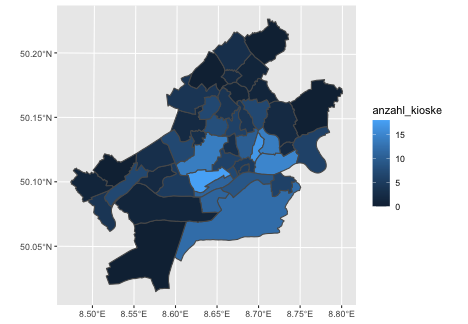
\includegraphics{_main_files/figure-latex/unnamed-chunk-98-1.png}

Allerdings wäre es schöner, die Kioskdichte (nach Fläche) darzustellen. Dazu berechnen wir zunächst die Flächen der Stadtteile:

\begin{Shaded}
\begin{Highlighting}[]
\FunctionTok{st\_area}\NormalTok{(stadtteile) }\SpecialCharTok{\%\textgreater{}\%}
  \FunctionTok{as.numeric}\NormalTok{() }\SpecialCharTok{/} \DecValTok{1000} \SpecialCharTok{/} \DecValTok{1000} \OtherTok{{-}\textgreater{}}
\NormalTok{  stadtteile}\SpecialCharTok{$}\NormalTok{qkm}
\end{Highlighting}
\end{Shaded}

Oder mit Pipes:

\begin{Shaded}
\begin{Highlighting}[]
\NormalTok{stadtteile }\SpecialCharTok{\%\textgreater{}\%}
  \FunctionTok{mutate}\NormalTok{(}\AttributeTok{qkm =} \FunctionTok{st\_area}\NormalTok{(.) }\SpecialCharTok{\%\textgreater{}\%} \FunctionTok{as.numeric}\NormalTok{() }\SpecialCharTok{/} \DecValTok{1000} \SpecialCharTok{/} \DecValTok{1000}\NormalTok{)}
\DocumentationTok{\#\# Simple feature collection with 46 features and 4 fields}
\DocumentationTok{\#\# geometry type:  POLYGON}
\DocumentationTok{\#\# dimension:      XY}
\DocumentationTok{\#\# bbox:           xmin: 462292.7 ymin: 5540412 xmax: 485744.8 ymax: 5563925}
\DocumentationTok{\#\# projected CRS:  ETRS89 / UTM zone 32N}
\DocumentationTok{\#\# First 10 features:}
\DocumentationTok{\#\#    STTLNR        STTLNAME}
\DocumentationTok{\#\# 1       1        Altstadt}
\DocumentationTok{\#\# 2       2      Innenstadt}
\DocumentationTok{\#\# 3       3 Bahnhofsviertel}
\DocumentationTok{\#\# 4       4     Westend{-}Süd}
\DocumentationTok{\#\# 5       5    Westend{-}Nord}
\DocumentationTok{\#\# 6       6    Nordend{-}West}
\DocumentationTok{\#\# 7       7     Nordend{-}Ost}
\DocumentationTok{\#\# 8       8          Ostend}
\DocumentationTok{\#\# 9       9        Bornheim}
\DocumentationTok{\#\# 10     10  Gutleutviertel}
\DocumentationTok{\#\#                          geometry anzahl\_kioske}
\DocumentationTok{\#\# 1  POLYGON ((476934.3 5550541,...             5}
\DocumentationTok{\#\# 2  POLYGON ((477611.9 5552034,...             5}
\DocumentationTok{\#\# 3  POLYGON ((475831 5550785, 4...             7}
\DocumentationTok{\#\# 4  POLYGON ((475745.4 5552373,...             6}
\DocumentationTok{\#\# 5  POLYGON ((476497.9 5553910,...             3}
\DocumentationTok{\#\# 6  POLYGON ((478362.5 5553898,...            10}
\DocumentationTok{\#\# 7  POLYGON ((478397.9 5551924,...            17}
\DocumentationTok{\#\# 8  POLYGON ((481955.2 5552141,...            15}
\DocumentationTok{\#\# 9  POLYGON ((478959.8 5552336,...            14}
\DocumentationTok{\#\# 10 POLYGON ((472942 5548802, 4...            11}
\DocumentationTok{\#\#          qkm}
\DocumentationTok{\#\# 1  0.5065673}
\DocumentationTok{\#\# 2  1.4902009}
\DocumentationTok{\#\# 3  0.5425421}
\DocumentationTok{\#\# 4  2.4948957}
\DocumentationTok{\#\# 5  1.6307925}
\DocumentationTok{\#\# 6  3.0977694}
\DocumentationTok{\#\# 7  1.5305338}
\DocumentationTok{\#\# 8  5.5573382}
\DocumentationTok{\#\# 9  2.7840413}
\DocumentationTok{\#\# 10 2.1982354}
\end{Highlighting}
\end{Shaded}

Und dann die Kioskdichte:

\begin{Shaded}
\begin{Highlighting}[]
\NormalTok{stadtteile }\SpecialCharTok{\%\textgreater{}\%}
  \FunctionTok{mutate}\NormalTok{(}\AttributeTok{qkm =} \FunctionTok{st\_area}\NormalTok{(.) }\SpecialCharTok{\%\textgreater{}\%} \FunctionTok{as.numeric}\NormalTok{() }\SpecialCharTok{/} \DecValTok{1000} \SpecialCharTok{/} \DecValTok{1000}\NormalTok{,}
         \AttributeTok{kioskdichte =}\NormalTok{ anzahl\_kioske }\SpecialCharTok{/}\NormalTok{ qkm)}
\DocumentationTok{\#\# Simple feature collection with 46 features and 5 fields}
\DocumentationTok{\#\# geometry type:  POLYGON}
\DocumentationTok{\#\# dimension:      XY}
\DocumentationTok{\#\# bbox:           xmin: 462292.7 ymin: 5540412 xmax: 485744.8 ymax: 5563925}
\DocumentationTok{\#\# projected CRS:  ETRS89 / UTM zone 32N}
\DocumentationTok{\#\# First 10 features:}
\DocumentationTok{\#\#    STTLNR        STTLNAME}
\DocumentationTok{\#\# 1       1        Altstadt}
\DocumentationTok{\#\# 2       2      Innenstadt}
\DocumentationTok{\#\# 3       3 Bahnhofsviertel}
\DocumentationTok{\#\# 4       4     Westend{-}Süd}
\DocumentationTok{\#\# 5       5    Westend{-}Nord}
\DocumentationTok{\#\# 6       6    Nordend{-}West}
\DocumentationTok{\#\# 7       7     Nordend{-}Ost}
\DocumentationTok{\#\# 8       8          Ostend}
\DocumentationTok{\#\# 9       9        Bornheim}
\DocumentationTok{\#\# 10     10  Gutleutviertel}
\DocumentationTok{\#\#                          geometry anzahl\_kioske}
\DocumentationTok{\#\# 1  POLYGON ((476934.3 5550541,...             5}
\DocumentationTok{\#\# 2  POLYGON ((477611.9 5552034,...             5}
\DocumentationTok{\#\# 3  POLYGON ((475831 5550785, 4...             7}
\DocumentationTok{\#\# 4  POLYGON ((475745.4 5552373,...             6}
\DocumentationTok{\#\# 5  POLYGON ((476497.9 5553910,...             3}
\DocumentationTok{\#\# 6  POLYGON ((478362.5 5553898,...            10}
\DocumentationTok{\#\# 7  POLYGON ((478397.9 5551924,...            17}
\DocumentationTok{\#\# 8  POLYGON ((481955.2 5552141,...            15}
\DocumentationTok{\#\# 9  POLYGON ((478959.8 5552336,...            14}
\DocumentationTok{\#\# 10 POLYGON ((472942 5548802, 4...            11}
\DocumentationTok{\#\#          qkm kioskdichte}
\DocumentationTok{\#\# 1  0.5065673    9.870357}
\DocumentationTok{\#\# 2  1.4902009    3.355252}
\DocumentationTok{\#\# 3  0.5425421   12.902225}
\DocumentationTok{\#\# 4  2.4948957    2.404910}
\DocumentationTok{\#\# 5  1.6307925    1.839596}
\DocumentationTok{\#\# 6  3.0977694    3.228129}
\DocumentationTok{\#\# 7  1.5305338   11.107236}
\DocumentationTok{\#\# 8  5.5573382    2.699134}
\DocumentationTok{\#\# 9  2.7840413    5.028661}
\DocumentationTok{\#\# 10 2.1982354    5.004014}
\end{Highlighting}
\end{Shaded}

Schließlich die Karte:

\begin{Shaded}
\begin{Highlighting}[]
\NormalTok{stadtteile }\SpecialCharTok{\%\textgreater{}\%}
  \FunctionTok{mutate}\NormalTok{(}\AttributeTok{qkm =} \FunctionTok{st\_area}\NormalTok{(.) }\SpecialCharTok{\%\textgreater{}\%} \FunctionTok{as.numeric}\NormalTok{() }\SpecialCharTok{/} \DecValTok{1000} \SpecialCharTok{/} \DecValTok{1000}\NormalTok{,}
         \AttributeTok{kioskdichte =}\NormalTok{ anzahl\_kioske }\SpecialCharTok{/}\NormalTok{ qkm) }\SpecialCharTok{\%\textgreater{}\%}
  \FunctionTok{ggplot}\NormalTok{() }\SpecialCharTok{+}
    \FunctionTok{geom\_sf}\NormalTok{(}\FunctionTok{aes}\NormalTok{(}\AttributeTok{fill =}\NormalTok{ kioskdichte), }\AttributeTok{color=}\ConstantTok{NA}\NormalTok{) }\SpecialCharTok{+}
    \FunctionTok{scale\_fill\_continuous}\NormalTok{(}\StringTok{"Kioske pro km²"}\NormalTok{) }\SpecialCharTok{+}
    \FunctionTok{theme\_void}\NormalTok{()}
\end{Highlighting}
\end{Shaded}

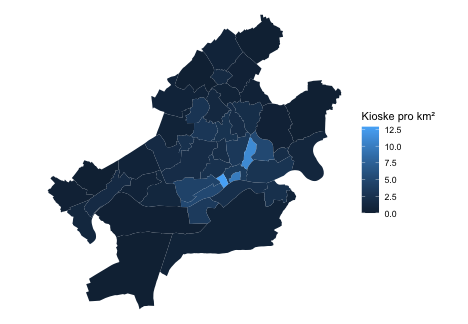
\includegraphics{_main_files/figure-latex/unnamed-chunk-102-1.png}

\hypertarget{aufgaben-4}{%
\subsection{Aufgaben}\label{aufgaben-4}}

\begin{enumerate}
\def\labelenumi{\arabic{enumi}.}
\item
  Erstellen Sie eine Choroplethenkarte der Frankfurter Stadtteile, in der Sie die Anzahl bzw. die Dichte von Apotheken darstellen. (Schritte analog zu oben.)
\item
  Welche Stadtteile haben mehr Kioske? Welche mehr Apotheken? Wie ausgeprägt ist das Verhältnis? Erstellen Sie eine Karte, die das zum Ausdruck bringt.
\item
  (Achtung, knifflig!) Siemens veröffentlicht einen \href{https://press.siemens.com/global/de/feature/wo-blitzt-es-am-haeufigsten}{Blitzatlas}. Laden Sie den Datensatz herunter und bauen Sie die folgende Ansicht nach:
\end{enumerate}

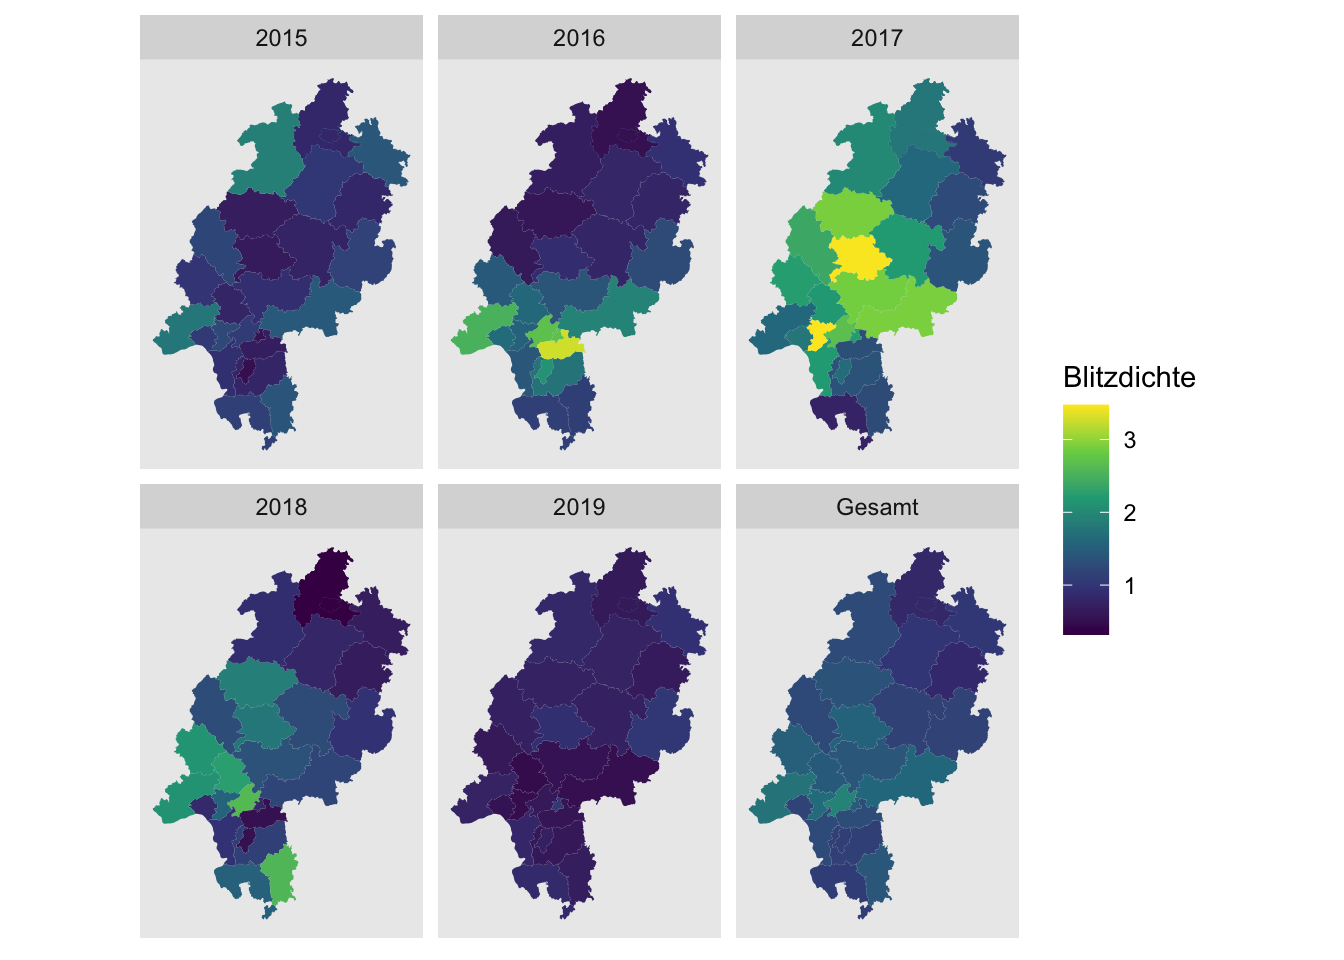
\includegraphics{_main_files/figure-latex/unnamed-chunk-105-1.png}

\hypertarget{text-chandra-2014}{%
\section{Text: Chandra 2014}\label{text-chandra-2014}}

\hypertarget{lesetext-2}{%
\subsection{Lesetext}\label{lesetext-2}}

Chandra, Vikram. 2014. \emph{Geek Sublime: The Beauty of Code, the Code of Beauty.} Graywolf Press, Minneapolis.

Daraus:

\begin{itemize}
\tightlist
\item
  Kapitel 1: Hello, World! (S. 1--8)
\item
  Kapitel 3: The Language of Logic (S. 19--40)
\end{itemize}

\hypertarget{fragen-an-den-text-2}{%
\subsection{Fragen an den Text}\label{fragen-an-den-text-2}}

\begin{enumerate}
\def\labelenumi{\arabic{enumi}.}
\tightlist
\item
  Um welche Art von Text handelt es sich? Wer ist der Autor, und an wen wendet er sich?
\item
  Was ist ``literate programming'', und was könnte das in R konkret bedeuten?
\item
  Auf S. 37 ist die Rede von ``our journey down the stack of languages''. Was ist damit gemeint?
\item
  Was findet der Autor an Code und Computern so faszinierend? Wo können Sie das nachvollziehen, und wo nicht?
\end{enumerate}

\hypertarget{themenfindung}{%
\subsection{Themenfindung}\label{themenfindung}}

\begin{itemize}
\tightlist
\item
  Bereiten Sie \emph{ein} Thema vor, zu dem Sie sich vorstellen könnten im Sommer zu arbeiten.
\item
  Achten Sie darauf, dass das Thema nicht zu allgemein ist (``Finanzmarkt'') aber auch nicht zu speziell (``Zusammenhang zwischen Quadratmeterzahl und Mietpreis für Ladenflächen in Ginnheim'').
\item
  Es wird in einem nächsten Schritt darum gehen, interessante Datenquellen zu finden (vielleicht haben Sie schon eine Idee?) und einer Fragestellung näher zu kommen.
\item
  Sie werden die Themen kurz vorstellen um Überschneidungen zu identifizieren und ggf. Gruppen zu bilden (wenn gewünscht).
\end{itemize}

\hypertarget{html-tabellen}{%
\section{HTML-Tabellen}\label{html-tabellen}}

\hypertarget{lernziele-dieser-sitzung-3}{%
\subsection{Lernziele dieser Sitzung}\label{lernziele-dieser-sitzung-3}}

Sie können\ldots{}

\begin{itemize}
\tightlist
\item
  sich den Quellcode einer Webseite anzeigen lassen und interpretieren.
\item
  HTML-Tabellen als Datensatz einlesen.
\item
  Fortgeschrittene Methoden der Datenbereinigung nachvollziehen.
\end{itemize}

\hypertarget{vorbereitung-2}{%
\subsection{Vorbereitung}\label{vorbereitung-2}}

Am Beispiel der Küstenlängen verschiedener Länder besprechen wir Techniken der Datenerhebung/-erfassung und -visualisierung. Unser Ziel ist es, die Daten zu den Küstenlängen in einer Grafik darzustellen.

Für die folgenden Aufgaben benötigen wir die Pakete \texttt{rvest} und \texttt{tidyverse}. Zunächst müssen diese installiert und in unsere Umgebung geladen werden.

\begin{Shaded}
\begin{Highlighting}[]
\FunctionTok{library}\NormalTok{(tidyverse)}
\FunctionTok{library}\NormalTok{(rvest)}
\end{Highlighting}
\end{Shaded}

\hypertarget{datenbeschaffung}{%
\subsection{Datenbeschaffung}\label{datenbeschaffung}}

Auf dem Internetauftritt der CIA gab es es eine Tabelle, welche die Küstenlänge (inklusive der Inseln) der einzelnen Länder enthält.

Über die Archivierungsplattform WayBackMachine ist die Seite immer noch abrufbar: \url{https://web.archive.org/web/20190802010710/https://www.cia.gov/library/publications/the-world-factbook/fields/282.html}

In einem ersten Schritt wird die URL der Tabelle der Variable \texttt{url} zugewiesen, sodass der Quellcode mit dem Befehl \texttt{read\_html()} eingelesen werden kann.

\begin{Shaded}
\begin{Highlighting}[]
\NormalTok{url }\OtherTok{\textless{}{-}} \StringTok{"https://web.archive.org/web/20190802010710/https://www.cia.gov/library/publications/the{-}world{-}factbook/fields/282.html"}
\NormalTok{reply }\OtherTok{\textless{}{-}} \FunctionTok{read\_html}\NormalTok{(url)}
\end{Highlighting}
\end{Shaded}

Der Befehl \texttt{html\_table()} ermöglicht das Auslesen \emph{aller} Tabellen auf der Seite. Mithilfe des Befehls \texttt{str()} sehen wir, dass die Seite genau eine Tabelle enthält, welche die Informationen zu den Küstenlängen enthält.

\begin{Shaded}
\begin{Highlighting}[]
\NormalTok{tables }\OtherTok{\textless{}{-}} \FunctionTok{html\_table}\NormalTok{(reply, }\AttributeTok{fill =} \ConstantTok{TRUE}\NormalTok{)}
\FunctionTok{str}\NormalTok{(tables)}
\DocumentationTok{\#\# List of 1}
\DocumentationTok{\#\#  $ :\textquotesingle{}data.frame\textquotesingle{}:    266 obs. of  2 variables:}
\DocumentationTok{\#\#   ..$ Country  : chr [1:266] "Afghanistan" "Akrotiri" "Albania" "Algeria" ...}
\DocumentationTok{\#\#   ..$ Coastline: chr [1:266] "0 km\textbackslash{}n          (landlocked)" "56.3 km" "362 km" "998 km" ...}
\end{Highlighting}
\end{Shaded}

Durch die Umformung zu einem tibble erhalten wir eine Tabelle mit den gewünschten Informationen:

\begin{Shaded}
\begin{Highlighting}[]
\FunctionTok{as\_tibble}\NormalTok{(tables[[}\DecValTok{1}\NormalTok{]])}
\DocumentationTok{\#\# \# A tibble: 266 x 2}
\DocumentationTok{\#\#    Country             Coastline                     }
\DocumentationTok{\#\#    \textless{}chr\textgreater{}               \textless{}chr\textgreater{}                         }
\DocumentationTok{\#\#  1 Afghanistan         "0 km\textbackslash{}n          (landlocked)"}
\DocumentationTok{\#\#  2 Akrotiri            "56.3 km"                     }
\DocumentationTok{\#\#  3 Albania             "362 km"                      }
\DocumentationTok{\#\#  4 Algeria             "998 km"                      }
\DocumentationTok{\#\#  5 American Samoa      "116 km"                      }
\DocumentationTok{\#\#  6 Andorra             "0 km\textbackslash{}n          (landlocked)"}
\DocumentationTok{\#\#  7 Angola              "1,600 km"                    }
\DocumentationTok{\#\#  8 Anguilla            "61 km"                       }
\DocumentationTok{\#\#  9 Antarctica          "17,968 km"                   }
\DocumentationTok{\#\# 10 Antigua and Barbuda "153 km"                      }
\DocumentationTok{\#\# \# ... with 256 more rows}
\end{Highlighting}
\end{Shaded}

Mit pipes können wir die obigen Befehle zusammenfassen und somit das Ganze auf einmal ausführen.

\begin{Shaded}
\begin{Highlighting}[]
\StringTok{"https://web.archive.org/web/20190802010710/https://www.cia.gov/library/publications/the{-}world{-}factbook/fields/282.html"} \SpecialCharTok{\%\textgreater{}\%}
  \FunctionTok{read\_html}\NormalTok{() }\SpecialCharTok{\%\textgreater{}\%}
  \FunctionTok{html\_table}\NormalTok{(}\AttributeTok{fill =}\NormalTok{ T) }\SpecialCharTok{\%\textgreater{}\%}
\NormalTok{  .[[}\DecValTok{1}\NormalTok{]] }\SpecialCharTok{\%\textgreater{}\%}
  \FunctionTok{as\_tibble}\NormalTok{() }\OtherTok{{-}\textgreater{}}\NormalTok{ coast}
\end{Highlighting}
\end{Shaded}

\hypertarget{datenformatierung}{%
\subsection{Datenformatierung}\label{datenformatierung}}

Zur Datenformatierung nutzen wir Funktionen aus dem Paket \texttt{stringr}. Die Spalte mit der Küstenlänge soll keinen Text, keine Einheit direkt hinter den Zahlenwerten und keine Kommata zur Trennung der Zahlenwerte enthalten.

Der Befehl ``str\_extract()'' sucht nach vorgegebenen Mustern (engl. \emph{patterns}) und wählt diese aus. Diese patterns werden auch reguläre Ausdrücke (\emph{regular expressions / regex}) genannt und sind eigentlich \href{https://danielfett.de/en/tutorials/tutorial-regulare-ausdrucke/}{ein Thema für sich}. Das Pattern \texttt{{[}0-9,.{]}+\ km} extrahiert die Kilometerangaben.

\begin{Shaded}
\begin{Highlighting}[]
\NormalTok{km }\OtherTok{\textless{}{-}} \FunctionTok{str\_extract}\NormalTok{(coast}\SpecialCharTok{$}\NormalTok{Coastline, }\StringTok{"[0{-}9,.]+ km"}\NormalTok{)}
\end{Highlighting}
\end{Shaded}

Die ausgewählten Muster (in unserem Fall Kommata und Text) können durch den Befehl \texttt{str\_replace\_all()} gelöscht oder ersetzt werden. Wir ersetzen alle Zeichen \emph{außer} Zahlen und Dezimalpunkt mit einem leeren String, so dass sie verschwinden.

\begin{Shaded}
\begin{Highlighting}[]
\FunctionTok{str\_replace\_all}\NormalTok{(km, }\StringTok{"[\^{}0{-}9.]"}\NormalTok{, }\StringTok{""}\NormalTok{)}
\DocumentationTok{\#\#   [1] "0"       "56.3"    "362"     "998"     "116"    }
\DocumentationTok{\#\#   [6] "0"       "1600"    "61"      "17968"   "153"    }
\DocumentationTok{\#\#  [11] "45389"   "4989"    "0"       "68.5"    "74.1"   }
\DocumentationTok{\#\#  [16] "111866"  "25760"   "0"       "0"       "3542"   }
\DocumentationTok{\#\#  [21] "161"     "580"     "97"      "0"       "66.5"   }
\DocumentationTok{\#\#  [26] "386"     "121"     "103"     "0"       "0"      }
\DocumentationTok{\#\#  [31] "20"      "0"       "29.6"    "7491"    "698"    }
\DocumentationTok{\#\#  [36] "80"      "161"     "354"     "0"       "1930"   }
\DocumentationTok{\#\#  [41] "0"       "965"     "443"     "402"     "202080" }
\DocumentationTok{\#\#  [46] "160"     "0"       "0"       "6435"    "14500"  }
\DocumentationTok{\#\#  [51] "138.9"   "11.1"    "26"      "3208"    "340"    }
\DocumentationTok{\#\#  [56] "37"      "169"     "120"     "3095"    "1290"   }
\DocumentationTok{\#\#  [61] "515"     "5835"    "3735"    "364"     "648"    }
\DocumentationTok{\#\#  [66] "0"       "7314"    "27.5"    "314"     "148"    }
\DocumentationTok{\#\#  [71] "1288"    "2237"    "2450"    "307"     "296"    }
\DocumentationTok{\#\#  [76] "2234"    "3794"    "0"       "0"       "65992.9"}
\DocumentationTok{\#\#  [81] "1288"    "1117"    "1129"    "1250"    "4853"   }
\DocumentationTok{\#\#  [86] "2525"    "28"      "885"     "80"      "40"     }
\DocumentationTok{\#\#  [91] "310"     "2389"    "539"     "12"      "13676"  }
\DocumentationTok{\#\#  [96] "44087"   "121"     "125.5"   "400"     "50"     }
\DocumentationTok{\#\# [101] "320"     "350"     "459"     "1771"    "101.9"  }
\DocumentationTok{\#\# [106] "0"       "823"     "733"     "6.4"     "0"      }
\DocumentationTok{\#\# [111] "4970"    "7000"    "66526"   "54716"   "2440"   }
\DocumentationTok{\#\# [116] "58"      "1448"    "160"     "273"     "7600"   }
\DocumentationTok{\#\# [121] "1022"    "124.1"   "29751"   "8"       "70"     }
\DocumentationTok{\#\# [126] "34"      "26"      "0"       "536"     "3"      }
\DocumentationTok{\#\# [131] "1143"    "2495"    "2413"    "0"       "499"    }
\DocumentationTok{\#\# [136] "0"       "0"       "498"     "225"     "0"      }
\DocumentationTok{\#\# [141] "579"     "1770"    "0"       "90"      "0"      }
\DocumentationTok{\#\# [146] "41"      "4828"    "0"       "4675"    "644"    }
\DocumentationTok{\#\# [151] "0"       "196.8"   "370.4"   "754"     "177"    }
\DocumentationTok{\#\# [156] "9330"    "6112"    "15"      "0"       "4.1"    }
\DocumentationTok{\#\# [161] "0"       "293.5"   "40"      "1835"    "2470"   }
\DocumentationTok{\#\# [166] "1572"    "30"      "8"       "0"       "451"    }
\DocumentationTok{\#\# [171] "2254"    "15134"   "910"     "0"       "853"    }
\DocumentationTok{\#\# [176] "64"      "32"      "0"       "1482"    "25148"  }
\DocumentationTok{\#\# [181] "2092"    "135663"  "1046"    "1519"    "14.5"   }
\DocumentationTok{\#\# [186] "2490"    "5152"    "518"     "0"       "2414"   }
\DocumentationTok{\#\# [191] "36289"   "51"      "440"     "1793"    "501"    }
\DocumentationTok{\#\# [196] "563"     "225"     "37653"   "0"       "60"     }
\DocumentationTok{\#\# [201] "135"     "158"     "58.9"    "120"     "84"     }
\DocumentationTok{\#\# [206] "403"     "0"       "209"     "2640"    "531"    }
\DocumentationTok{\#\# [211] "0"       "491"     "402"     "193"     "58.9"   }
\DocumentationTok{\#\# [216] "0"       "46.6"    "5313"    "3025"    "2798"   }
\DocumentationTok{\#\# [221] NA        "0"       "17968"   "4964"    "926"    }
\DocumentationTok{\#\# [226] "1340"    "853"     "386"     "3587"    "3218"   }
\DocumentationTok{\#\# [231] "0"       "193"     "1566.3"  "0"       "1424"   }
\DocumentationTok{\#\# [236] "3219"    "706"     "56"      "101"     "419"    }
\DocumentationTok{\#\# [241] "362"     "1148"    "7200"    "0"       "389"    }
\DocumentationTok{\#\# [246] "24"      "0"       "2782"    "1318"    "12429"  }
\DocumentationTok{\#\# [251] "19924"   "4.8"     "660"     "0"       "2528"   }
\DocumentationTok{\#\# [256] "2800"    "3444"    "188"     "19.3"    "129"    }
\DocumentationTok{\#\# [261] "0"       "1110"    "356000"  "1906"    "0"      }
\DocumentationTok{\#\# [266] "0"}
\end{Highlighting}
\end{Shaded}

Auch hier kann alles in einen Befehl gepackt werden:

\begin{Shaded}
\begin{Highlighting}[]
\NormalTok{coast}\SpecialCharTok{$}\NormalTok{Coastline }\SpecialCharTok{\%\textgreater{}\%}
  \FunctionTok{str\_extract}\NormalTok{(}\StringTok{"[0{-}9,.]+ km"}\NormalTok{) }\SpecialCharTok{\%\textgreater{}\%}
  \FunctionTok{str\_replace\_all}\NormalTok{(}\StringTok{"[\^{}0{-}9.]"}\NormalTok{, }\StringTok{""}\NormalTok{) }\SpecialCharTok{\%\textgreater{}\%}
  \FunctionTok{as.numeric}\NormalTok{() }\OtherTok{{-}\textgreater{}}\NormalTok{ coast}\SpecialCharTok{$}\NormalTok{coast\_num}
\end{Highlighting}
\end{Shaded}

\hypertarget{datenaufbereitung}{%
\subsection{Datenaufbereitung}\label{datenaufbereitung}}

Mit dem Befehl \texttt{arrange()} kann die Tabelle sortiert werden. Zunächst auftseigend,

\begin{Shaded}
\begin{Highlighting}[]
\NormalTok{coast }\SpecialCharTok{\%\textgreater{}\%}
  \FunctionTok{arrange}\NormalTok{(coast\_num)}
\DocumentationTok{\#\# \# A tibble: 266 x 3}
\DocumentationTok{\#\#    Country    Coastline                       coast\_num}
\DocumentationTok{\#\#    \textless{}chr\textgreater{}      \textless{}chr\textgreater{}                               \textless{}dbl\textgreater{}}
\DocumentationTok{\#\#  1 Afghanist\textasciitilde{} "0 km\textbackslash{}n          (landlocked)"          0}
\DocumentationTok{\#\#  2 Andorra    "0 km\textbackslash{}n          (landlocked)"          0}
\DocumentationTok{\#\#  3 Armenia    "0 km\textbackslash{}n          (landlocked)"          0}
\DocumentationTok{\#\#  4 Austria    "0 km\textbackslash{}n          (landlocked)"          0}
\DocumentationTok{\#\#  5 Azerbaijan "0 km\textbackslash{}n          (landlocked);\textasciitilde{}         0}
\DocumentationTok{\#\#  6 Belarus    "0 km\textbackslash{}n          (landlocked)"          0}
\DocumentationTok{\#\#  7 Bhutan     "0 km\textbackslash{}n          (landlocked)"          0}
\DocumentationTok{\#\#  8 Bolivia    "0 km\textbackslash{}n          (landlocked)"          0}
\DocumentationTok{\#\#  9 Botswana   "0 km\textbackslash{}n          (landlocked)"          0}
\DocumentationTok{\#\# 10 Burkina F\textasciitilde{} "0 km\textbackslash{}n          (landlocked)"          0}
\DocumentationTok{\#\# \# ... with 256 more rows}
\end{Highlighting}
\end{Shaded}

und schließlich absteigend, sodass die größten Werte an erster Stelle stehen.

\begin{Shaded}
\begin{Highlighting}[]
\NormalTok{coast }\SpecialCharTok{\%\textgreater{}\%}
  \FunctionTok{arrange}\NormalTok{(}\FunctionTok{desc}\NormalTok{(coast\_num))}
\DocumentationTok{\#\# \# A tibble: 266 x 3}
\DocumentationTok{\#\#    Country     Coastline                      coast\_num}
\DocumentationTok{\#\#    \textless{}chr\textgreater{}       \textless{}chr\textgreater{}                              \textless{}dbl\textgreater{}}
\DocumentationTok{\#\#  1 World       "356,000 km\textbackslash{}n          \textbackslash{}n    \textasciitilde{}   356000 }
\DocumentationTok{\#\#  2 Canada      "202,080 km\textbackslash{}n          \textbackslash{}n    \textasciitilde{}   202080 }
\DocumentationTok{\#\#  3 Pacific Oc\textasciitilde{} "135,663 km"                     135663 }
\DocumentationTok{\#\#  4 Atlantic O\textasciitilde{} "111,866 km"                     111866 }
\DocumentationTok{\#\#  5 Indian Oce\textasciitilde{} "66,526 km"                       66526 }
\DocumentationTok{\#\#  6 European U\textasciitilde{} "65,992.9 km"                     65993.}
\DocumentationTok{\#\#  7 Indonesia   "54,716 km"                       54716 }
\DocumentationTok{\#\#  8 Arctic Oce\textasciitilde{} "45,389 km"                       45389 }
\DocumentationTok{\#\#  9 Greenland   "44,087 km"                       44087 }
\DocumentationTok{\#\# 10 Russia      "37,653 km"                       37653 }
\DocumentationTok{\#\# \# ... with 256 more rows}
\end{Highlighting}
\end{Shaded}

Bevor wir jedoch eine vollständig sortierte Liste haben, muss der Datensatz noch von falschen Einträgen gesäubert werden. Dafür benutzen wir den Befehl \texttt{filter()}. Wir suchen wieder nach einem bestimmten Muster (hier zum Beispiel dem Wort ``Ocean'') und filtern es aus dem Datensatz.

Die Grafik soll nur aus den ersten 30 Einträgen der Tabelle bestehen, welche uns der Befehl \texttt{head()} ausgibt.

\begin{Shaded}
\begin{Highlighting}[]
\NormalTok{coast }\SpecialCharTok{\%\textgreater{}\%}
  \FunctionTok{arrange}\NormalTok{(}\FunctionTok{desc}\NormalTok{(coast\_num)) }\SpecialCharTok{\%\textgreater{}\%}
  \FunctionTok{filter}\NormalTok{(}\SpecialCharTok{!}\FunctionTok{str\_detect}\NormalTok{(Country, }\StringTok{"Ocean"}\NormalTok{)) }\SpecialCharTok{\%\textgreater{}\%}
  \FunctionTok{filter}\NormalTok{(}\SpecialCharTok{!}\NormalTok{Country }\SpecialCharTok{\%in\%} \FunctionTok{c}\NormalTok{(}\StringTok{"World"}\NormalTok{, }\StringTok{"European Union"}\NormalTok{)) }\SpecialCharTok{\%\textgreater{}\%}
  \FunctionTok{head}\NormalTok{(}\DecValTok{30}\NormalTok{) }\OtherTok{{-}\textgreater{}}\NormalTok{ top\_30}
\end{Highlighting}
\end{Shaded}

\hypertarget{datenvisualisierung}{%
\subsection{Datenvisualisierung}\label{datenvisualisierung}}

Das Balkendiagramm erhalten wir durch den ``ggplot'' Befehl. Hierbei gibt es verschiedenste Einstellmöglichkeiten. Wichitg sind vor allem die Angabe des verwendeten Datensatzes und die Art der Grafik (ob Kartendarstellung oder Balkendiagramm). Desweiteren kann man noch Farben der Eigenschaften, eine Achsenbeschriftung u. v. m. bestimmen.

\begin{Shaded}
\begin{Highlighting}[]
\FunctionTok{ggplot}\NormalTok{(top\_30, }\FunctionTok{aes}\NormalTok{(}\AttributeTok{x =} \FunctionTok{reorder}\NormalTok{(Country, coast\_num), }\AttributeTok{y=}\NormalTok{coast\_num)) }\SpecialCharTok{+}
  \FunctionTok{geom\_bar}\NormalTok{(}\AttributeTok{stat=}\StringTok{\textquotesingle{}identity\textquotesingle{}}\NormalTok{, }\AttributeTok{fill=}\StringTok{"darkblue"}\NormalTok{) }\SpecialCharTok{+}
  \FunctionTok{coord\_flip}\NormalTok{() }\SpecialCharTok{+}
  \FunctionTok{scale\_x\_discrete}\NormalTok{(}\ConstantTok{NULL}\NormalTok{) }\SpecialCharTok{+}
  \FunctionTok{scale\_y\_continuous}\NormalTok{(}\StringTok{"Küstenlinie (km)"}\NormalTok{)}
\end{Highlighting}
\end{Shaded}

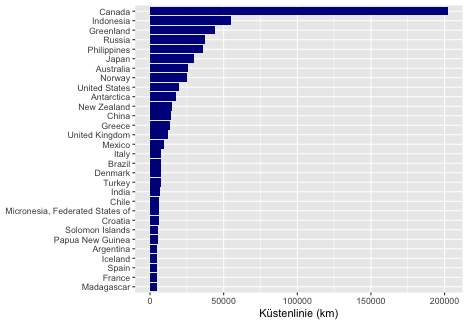
\includegraphics{_main_files/figure-latex/unnamed-chunk-117-1.png}

\hypertarget{aufgaben-5}{%
\subsection{Aufgaben}\label{aufgaben-5}}

\begin{enumerate}
\def\labelenumi{\arabic{enumi}.}
\tightlist
\item
  Importieren Sie die Daten zu den \href{https://en.wikipedia.org/wiki/List_of_deadly_earthquakes_since_1900}{tödlichen Erdbeben auf Wikipedia}
  und formen sie diese zu einem tibble um.
\end{enumerate}

\begin{Shaded}
\begin{Highlighting}[]
\StringTok{"https://en.wikipedia.org/wiki/List\_of\_deadly\_earthquakes\_since\_1900"} \SpecialCharTok{\%\textgreater{}\%}
\NormalTok{  read\_html }\SpecialCharTok{\%\textgreater{}\%}
  \FunctionTok{html\_table}\NormalTok{(}\AttributeTok{fill =}\NormalTok{ T) }\SpecialCharTok{\%\textgreater{}\%}
\NormalTok{  .[[}\DecValTok{5}\NormalTok{]] }\SpecialCharTok{\%\textgreater{}\%}
  \FunctionTok{as.tibble}\NormalTok{() }\OtherTok{{-}\textgreater{}}\NormalTok{ earthquakes\_raw}
\end{Highlighting}
\end{Shaded}

\begin{enumerate}
\def\labelenumi{\arabic{enumi}.}
\setcounter{enumi}{1}
\tightlist
\item
  Erstellen Sie mit den erhaltenen Daten eine Karte, welche die Lage und die Stärke der Erdbeben angibt:
\end{enumerate}

\begin{Shaded}
\begin{Highlighting}[]
\NormalTok{earthquakes\_raw }\SpecialCharTok{\%\textgreater{}\%}
  \FunctionTok{mutate}\NormalTok{(}\AttributeTok{Lat =} \FunctionTok{as.numeric}\NormalTok{(Lat), }\AttributeTok{Long =} \FunctionTok{as.numeric}\NormalTok{(Long)) }\SpecialCharTok{\%\textgreater{}\%}
  \FunctionTok{mutate}\NormalTok{(}\AttributeTok{magnitude\_num =} \FunctionTok{as.numeric}\NormalTok{(}\FunctionTok{str\_extract}\NormalTok{(Magnitude, }\StringTok{"[0{-}9.]+"}\NormalTok{))) }\OtherTok{{-}\textgreater{}}\NormalTok{ earthquakes}

\FunctionTok{ggplot}\NormalTok{() }\SpecialCharTok{+}
  \FunctionTok{geom\_polygon}\NormalTok{(}\AttributeTok{data =} \FunctionTok{map\_data}\NormalTok{(}\StringTok{"world"}\NormalTok{), }\FunctionTok{aes}\NormalTok{(}\AttributeTok{x =}\NormalTok{ long, }\AttributeTok{y =}\NormalTok{ lat, }\AttributeTok{group =}\NormalTok{ group)) }\SpecialCharTok{+}
  \FunctionTok{geom\_point}\NormalTok{(}\AttributeTok{data =}\NormalTok{ earthquakes,}
             \FunctionTok{aes}\NormalTok{(}\AttributeTok{x =}\NormalTok{ Long, }\AttributeTok{y =}\NormalTok{ Lat, }\AttributeTok{size =}\NormalTok{ magnitude\_num),}
             \AttributeTok{color =} \StringTok{"red"}\NormalTok{, }\AttributeTok{alpha =} \FloatTok{0.1}\NormalTok{) }\SpecialCharTok{+}
  \FunctionTok{coord\_quickmap}\NormalTok{() }\SpecialCharTok{+}
  \FunctionTok{scale\_size\_area}\NormalTok{(}\StringTok{"Stärke"}\NormalTok{)}
\end{Highlighting}
\end{Shaded}

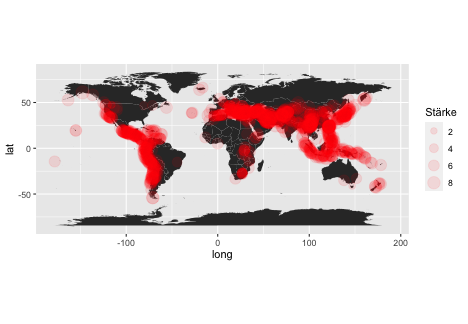
\includegraphics{_main_files/figure-latex/unnamed-chunk-120-1.png}

\begin{enumerate}
\def\labelenumi{\arabic{enumi}.}
\setcounter{enumi}{2}
\tightlist
\item
  Wandeln Sie den Erdbeben-Datensatz in das Simple Features Format um. Laden Sie zusätzlich eine Weltkarte mit dem Paket \texttt{rnaturalearth} und wandeln Sie auch diese in Simple Features um. Finden Sie außerdem einen Geodatensatz zu tektonischen Platten. Visualiseren Sie alles auf einer Welktarte (Projektion: Gall-Peters).
\end{enumerate}

\begin{Shaded}
\begin{Highlighting}[]
\FunctionTok{library}\NormalTok{(sf)}

\NormalTok{earthquakes }\SpecialCharTok{\%\textgreater{}\%}
  \FunctionTok{filter}\NormalTok{(}\SpecialCharTok{!} \FunctionTok{is.na}\NormalTok{(Long)) }\SpecialCharTok{\%\textgreater{}\%}
  \FunctionTok{st\_as\_sf}\NormalTok{(}\AttributeTok{coords=}\FunctionTok{c}\NormalTok{(}\StringTok{"Long"}\NormalTok{, }\StringTok{"Lat"}\NormalTok{)) }\SpecialCharTok{\%\textgreater{}\%}
  \FunctionTok{st\_set\_crs}\NormalTok{(}\DecValTok{4326}\NormalTok{) }\OtherTok{{-}\textgreater{}}\NormalTok{ quakesf}

\FunctionTok{library}\NormalTok{(rnaturalearth)}

\FunctionTok{ne\_download}\NormalTok{(}\AttributeTok{type=}\StringTok{"land"}\NormalTok{, }\AttributeTok{category =} \StringTok{"physical"}\NormalTok{) }\SpecialCharTok{\%\textgreater{}\%}
  \FunctionTok{st\_as\_sf}\NormalTok{() }\SpecialCharTok{\%\textgreater{}\%}
  \FunctionTok{st\_transform}\NormalTok{(}\StringTok{\textquotesingle{}+proj=cea +lon\_0=0 +x\_0=0 +y\_0=0 +lat\_ts=45 +ellps=WGS84 +datum=WGS84 +units=m +no\_defs\textquotesingle{}}\NormalTok{) }\OtherTok{{-}\textgreater{}}\NormalTok{ earthsf}

\FunctionTok{st\_read}\NormalTok{(}\StringTok{"https://raw.githubusercontent.com/fraxen/tectonicplates/master/GeoJSON/PB2002\_plates.json"}\NormalTok{) }\OtherTok{{-}\textgreater{}}\NormalTok{ plates}

\FunctionTok{ggplot}\NormalTok{() }\SpecialCharTok{+}
  \FunctionTok{geom\_sf}\NormalTok{(}\AttributeTok{data =}\NormalTok{ earthsf, }\AttributeTok{fill =} \StringTok{"gray"}\NormalTok{, }\AttributeTok{color =} \ConstantTok{NA}\NormalTok{) }\SpecialCharTok{+}
  \FunctionTok{geom\_sf}\NormalTok{(}\AttributeTok{size =} \DecValTok{1}\NormalTok{, }\AttributeTok{data =}\NormalTok{ quakesf, }\AttributeTok{color =} \StringTok{"red"}\NormalTok{, }\AttributeTok{alpha =} \FloatTok{0.1}\NormalTok{) }\SpecialCharTok{+}
  \FunctionTok{geom\_sf}\NormalTok{(}\AttributeTok{data =}\NormalTok{ plates, }\AttributeTok{color =} \StringTok{"orange"}\NormalTok{, }\AttributeTok{fill =} \ConstantTok{NA}\NormalTok{, }\AttributeTok{lwd =} \FloatTok{0.3}\NormalTok{)}
\end{Highlighting}
\end{Shaded}

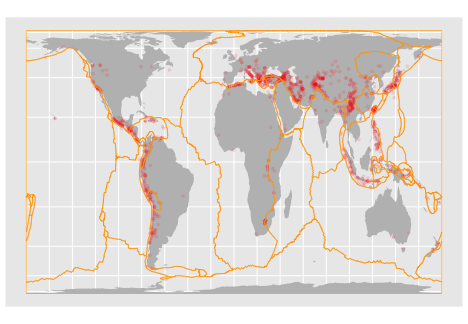
\includegraphics{_main_files/figure-latex/unnamed-chunk-123-1.png}

\hypertarget{web-scraping}{%
\section{Web scraping}\label{web-scraping}}

\hypertarget{lernziele-dieser-sitzung-4}{%
\subsection{Lernziele dieser Sitzung}\label{lernziele-dieser-sitzung-4}}

Sie können\ldots{}

\begin{itemize}
\tightlist
\item
  HTML in seiner Grundstruktur interpretieren.
\item
  gezielt einzelne Elemente einer Seite mit R auslesen.
\end{itemize}

\hypertarget{vorbereitung-3}{%
\subsection{Vorbereitung}\label{vorbereitung-3}}

Für diese Lektion werden folgende Pakete benötigt:

\begin{Shaded}
\begin{Highlighting}[]
\FunctionTok{library}\NormalTok{(tidyverse)}
\FunctionTok{library}\NormalTok{(rvest)}
\end{Highlighting}
\end{Shaded}

\hypertarget{exkurs-html}{%
\subsection{Exkurs: HTML}\label{exkurs-html}}

Wenn man eine Webseite ganz normal in einem Browser aufruft, erscheint sie als eine Mischung aus formatiertem Text, Bildern, Designelementen, ggf. Videos, usw. Was aber im Hintergrund eigentlich vom Server an den Browser übertragen wird, ist eine Textdatei in einem bestimmten Format -- HTML (Hyptertext Markup Language). Darin wird Text auf eine genau festgelegte Art und Weise annotiert, damit der Browser weiß, wie er ihn anzeigen soll. Im HTML-Dokument kann auch stehen: Lade ein Bild von einer bestimmten Stelle und zeig es an dieser Stelle an.

Einen brauchbaren Überblick über die HTML-Elemente und die Struktur einer HTML-Datei gibt es hier: \url{https://www.tutorialspoint.com/de/html/}

An dieser Stelle ist wichtig ist zu wissen: HTML-Elemente (``Tags'' oder ``Nodes'') sind streng hierarchisch angeordnet. Sie bestehen oft aus einem Anfangs- und einem End-Tag in spitzen Klammern:

\begin{verbatim}
<html>
  <head>
    <title>Titel meiner Webseite</title>
  </head>
  <body>
    <h1>Überschrift</h1>
    <p>Erster Absatz mit <b>fettem Text</b></p>
    <p>Zweiter Absatz mit <i>kursivem Text</i></p>
    <img src="path/to/image.jpg alt="Ein Bild" />
  </body>
</html>
\end{verbatim}

In diesem Beispiel ist das Bild mit \texttt{\textless{}img\ /\textgreater{}} das einzige Element, das nicht geöffnet und wieder geschlossen wird. Außerdem hat dieses Element Attribute (\texttt{src} und \texttt{alt}) mit bestimmten Werten. Eine echte Webseite ist weitaus komplexer und unübersichtlicher.

Dem Browser kann man sagen: Zeig mir nicht wie üblich die „gerenderte`` Seite an, sondern die zu Grunde liegende HTML-Datei. Das geht mit „Quelltext anzeigen`` / „View Source`` o.ä.

Viele Browser (hier seien Chrome und Firefox empfohlen) haben auch einen Modus namens „Entwicklertools`` / „Developer tools``, in dem die HTML-Elemente hierarchisch geordnet sind.

\hypertarget{seite-laden}{%
\subsection{Seite laden}\label{seite-laden}}

Beim so genannten Web Scraping ist die Grundidee, dass wir eine Webseite nicht im Browser öffnen, sondern den HTML-Quelltext direkt in R laden. R kann dann aus dem Quelltext bestimmte Elemente extrahieren.

In der letzten Sitzung haben wir schon gesehen, wie Tabellen nach genau diesem Prinzip von einer Webseite direkt in R geladen werden können. Jetzt soll es darum gehen, noch präziser zu sagen, welche Elemente wir von einer bestimmten Webseite ziehen wollen.

Als Beispiel soll die Infoseite eines Wohnheims des Studentenwerks Frankfurt dienen. Die Adresse ist: \url{https://www.studentenwerkfrankfurt.de/wohnen/wohnheime/frankfurt-am-main/kleine-seestrasse-11}

Zunächst laden wir den Quelltext in R und nennen ihn \texttt{quelltext}:

\begin{Shaded}
\begin{Highlighting}[]
\NormalTok{quelltext }\OtherTok{\textless{}{-}} \FunctionTok{read\_html}\NormalTok{(}\StringTok{"https://www.studentenwerkfrankfurt.de/wohnen/wohnheime/frankfurt{-}am{-}main/kleine{-}seestrasse{-}11"}\NormalTok{)}

\NormalTok{quelltext}
\DocumentationTok{\#\# \{html\_document\}}
\DocumentationTok{\#\# \textless{}html lang="de" dir="ltr" class="no{-}js"\textgreater{}}
\DocumentationTok{\#\# [1] \textless{}head\textgreater{}\textbackslash{}n\textless{}meta http{-}equiv="Content{-}Type" content= ...}
\DocumentationTok{\#\# [2] \textless{}body id="p187" class="page{-}187 pagelevel{-}4 lang ...}
\end{Highlighting}
\end{Shaded}

In diesem Schritt hat R den HTML-Quelltext schon ``geparsed'', d.h. ihn nicht nur als Text gespeichert, sondern als hierarchische Konstruktion mit den beiden Grundelementen \texttt{head} und \texttt{html}.

\hypertarget{elemente-suchen}{%
\subsection{Elemente suchen}\label{elemente-suchen}}

Uns soll jetzt das Baujahr interessieren. Auf der Seite stehen die Informationen rechts neben dem Bild. Mit den Entwicklertools können wir schauen, wie die Elemente in HTML genau heißen. Ein geeigneter Ausgangspunkt wäre das \texttt{\textless{}div\textgreater{}}-Element mit dem Attribut \texttt{id="c599"}.

In R können wir dieses einzelne Element ansprechen mit:

\begin{Shaded}
\begin{Highlighting}[]
\NormalTok{quelltext }\SpecialCharTok{\%\textgreater{}\%}
  \FunctionTok{html\_node}\NormalTok{(}\StringTok{"div\#c599"}\NormalTok{)}
\DocumentationTok{\#\# \{html\_node\}}
\DocumentationTok{\#\# \textless{}div id="c599" class="frame frame{-}default frame{-}type{-}text frame{-}layout{-}0 frame{-}background{-}none frame{-}no{-}backgroundimage frame{-}space{-}before{-}none frame{-}space{-}after{-}none"\textgreater{}}
\DocumentationTok{\#\# [1] \textless{}div class="frame{-}container"\textgreater{}\textless{}div class="frame{-}i ...}
\end{Highlighting}
\end{Shaded}

Dann gehen wir in der Hierarchie drei \texttt{\textless{}div\textgreater{}}- Elemente „tiefer``. (\texttt{\textless{}div\textgreater{}}- Elemente sind abstrakte Container und werden im Webdesign oft angewendet.)

\begin{Shaded}
\begin{Highlighting}[]
\NormalTok{quelltext }\SpecialCharTok{\%\textgreater{}\%}
  \FunctionTok{html\_node}\NormalTok{(}\StringTok{"div\#c599"}\NormalTok{) }\SpecialCharTok{\%\textgreater{}\%}
  \FunctionTok{html\_node}\NormalTok{(}\StringTok{"div"}\NormalTok{) }\SpecialCharTok{\%\textgreater{}\%}
  \FunctionTok{html\_node}\NormalTok{(}\StringTok{"div"}\NormalTok{)}
\DocumentationTok{\#\# \{html\_node\}}
\DocumentationTok{\#\# \textless{}div class="frame{-}inner"\textgreater{}}
\DocumentationTok{\#\# [1] \textless{}p\textgreater{}Kleine Seestraße 11\textless{}br\textgreater{}60486 Frankfurt am Mai ...}
\DocumentationTok{\#\# [2] \textless{}p\textgreater{}25 Wohnheimplätze\textless{}/p\textgreater{}\textbackslash{}n}
\DocumentationTok{\#\# [3] \textless{}ul class="list{-}normal"\textgreater{}\textbackslash{}n\textless{}li\textgreater{}5 Wohnküchen\textless{}/li\textgreater{}\textbackslash{} ...}
\DocumentationTok{\#\# [4] \textless{}p\textgreater{}Baujahr\textless{}strong\textgreater{} \textless{}/strong\textgreater{}1995\textbackslash{}r\textless{}/p\textgreater{}\textbackslash{}n}
\DocumentationTok{\#\# [5] \textless{}p\textgreater{}\textless{}strong\textgreater{}\textless{}/strong\textgreater{}\textless{}/p\textgreater{}}
\end{Highlighting}
\end{Shaded}

Alternativ könnten wir auch sagen: Darin das \texttt{div} mit \texttt{class="frame-inner"}:

\begin{Shaded}
\begin{Highlighting}[]
\NormalTok{quelltext }\SpecialCharTok{\%\textgreater{}\%}
  \FunctionTok{html\_node}\NormalTok{(}\StringTok{"div\#c599"}\NormalTok{) }\SpecialCharTok{\%\textgreater{}\%}
  \FunctionTok{html\_node}\NormalTok{(}\StringTok{"div.frame{-}inner"}\NormalTok{)}
\DocumentationTok{\#\# \{html\_node\}}
\DocumentationTok{\#\# \textless{}div class="frame{-}inner"\textgreater{}}
\DocumentationTok{\#\# [1] \textless{}p\textgreater{}Kleine Seestraße 11\textless{}br\textgreater{}60486 Frankfurt am Mai ...}
\DocumentationTok{\#\# [2] \textless{}p\textgreater{}25 Wohnheimplätze\textless{}/p\textgreater{}\textbackslash{}n}
\DocumentationTok{\#\# [3] \textless{}ul class="list{-}normal"\textgreater{}\textbackslash{}n\textless{}li\textgreater{}5 Wohnküchen\textless{}/li\textgreater{}\textbackslash{} ...}
\DocumentationTok{\#\# [4] \textless{}p\textgreater{}Baujahr\textless{}strong\textgreater{} \textless{}/strong\textgreater{}1995\textbackslash{}r\textless{}/p\textgreater{}\textbackslash{}n}
\DocumentationTok{\#\# [5] \textless{}p\textgreater{}\textless{}strong\textgreater{}\textless{}/strong\textgreater{}\textless{}/p\textgreater{}}
\end{Highlighting}
\end{Shaded}

mit \texttt{html\_nodes()} (Mehrzahl) werden alle Unterelemente eines Typs (hier \texttt{\textless{}p\textgreater{}} = Paragraph) angesprochen. Davon dann den Textinhalt (\texttt{html\_text()}) gibt uns die relevanten Informationen:

\begin{Shaded}
\begin{Highlighting}[]
\NormalTok{quelltext }\SpecialCharTok{\%\textgreater{}\%}
  \FunctionTok{html\_node}\NormalTok{(}\StringTok{"div\#c599"}\NormalTok{) }\SpecialCharTok{\%\textgreater{}\%}
  \FunctionTok{html\_node}\NormalTok{(}\StringTok{"div.frame{-}inner"}\NormalTok{) }\SpecialCharTok{\%\textgreater{}\%}
  \FunctionTok{html\_nodes}\NormalTok{(}\StringTok{"p"}\NormalTok{) }\SpecialCharTok{\%\textgreater{}\%}
  \FunctionTok{html\_text}\NormalTok{()}
\DocumentationTok{\#\# [1] "Kleine Seestraße 1160486 Frankfurt am Main\textbackslash{}r"}
\DocumentationTok{\#\# [2] "25 Wohnheimplätze"                           }
\DocumentationTok{\#\# [3] "Baujahr 1995\textbackslash{}r"                              }
\DocumentationTok{\#\# [4] ""}
\end{Highlighting}
\end{Shaded}

\hypertarget{elemente-reinigen}{%
\subsection{Elemente reinigen}\label{elemente-reinigen}}

Jetzt ließe sich der dritte Eintrag dieses Ergebnisvectors reinigen und als Ergebnis ``speichern''.

Der Befehl \texttt{str\_extract()} wendet dabei einen Regulären Ausdruck an, der nach einer Folge von vier Zahlen sucht.

\begin{Shaded}
\begin{Highlighting}[]
\NormalTok{quelltext }\SpecialCharTok{\%\textgreater{}\%}
  \FunctionTok{html\_node}\NormalTok{(}\StringTok{"div\#c599"}\NormalTok{) }\SpecialCharTok{\%\textgreater{}\%}
  \FunctionTok{html\_node}\NormalTok{(}\StringTok{"div.frame{-}inner"}\NormalTok{) }\SpecialCharTok{\%\textgreater{}\%}
  \FunctionTok{html\_nodes}\NormalTok{(}\StringTok{"p"}\NormalTok{) }\SpecialCharTok{\%\textgreater{}\%}
  \FunctionTok{html\_text}\NormalTok{() }\SpecialCharTok{\%\textgreater{}\%}
\NormalTok{  .[}\DecValTok{3}\NormalTok{] }\SpecialCharTok{\%\textgreater{}\%}
  \FunctionTok{str\_extract}\NormalTok{(}\StringTok{"[0{-}9]\{4\}"}\NormalTok{) }\SpecialCharTok{\%\textgreater{}\%}
  \FunctionTok{as.numeric}\NormalTok{() }\OtherTok{{-}\textgreater{}}\NormalTok{ baujahr}

\NormalTok{baujahr}
\DocumentationTok{\#\# [1] 1995}
\end{Highlighting}
\end{Shaded}

Wie diese Technik automatisiert auf eine Reihe von Seiten angewendet werden kann, wird zu einem späteren Zeitpunkt besprochen.

\hypertarget{aufgaben-6}{%
\subsection{Aufgaben}\label{aufgaben-6}}

\begin{enumerate}
\def\labelenumi{\arabic{enumi}.}
\tightlist
\item
  Lesen Sie die Anzahl der Wohnheimplätze aus.
\end{enumerate}

\begin{Shaded}
\begin{Highlighting}[]
\NormalTok{quelltext}
\DocumentationTok{\#\# \{html\_document\}}
\DocumentationTok{\#\# \textless{}html lang="de" dir="ltr" class="no{-}js"\textgreater{}}
\DocumentationTok{\#\# [1] \textless{}head\textgreater{}\textbackslash{}n\textless{}meta http{-}equiv="Content{-}Type" content= ...}
\DocumentationTok{\#\# [2] \textless{}body id="p187" class="page{-}187 pagelevel{-}4 lang ...}
\end{Highlighting}
\end{Shaded}

\begin{Shaded}
\begin{Highlighting}[]
\NormalTok{quelltext }\SpecialCharTok{\%\textgreater{}\%}
  \FunctionTok{html\_node}\NormalTok{(}\StringTok{"div\#c599"}\NormalTok{) }\SpecialCharTok{\%\textgreater{}\%}
  \FunctionTok{html\_node}\NormalTok{(}\StringTok{"div.frame{-}inner"}\NormalTok{) }\SpecialCharTok{\%\textgreater{}\%}
  \FunctionTok{html\_nodes}\NormalTok{(}\StringTok{"p"}\NormalTok{) }\SpecialCharTok{\%\textgreater{}\%}
  \FunctionTok{html\_text}\NormalTok{() }\SpecialCharTok{\%\textgreater{}\%}
\NormalTok{  .[}\DecValTok{2}\NormalTok{] }\SpecialCharTok{\%\textgreater{}\%}
  \FunctionTok{str\_extract}\NormalTok{(}\StringTok{"[0{-}9]+"}\NormalTok{) }\SpecialCharTok{\%\textgreater{}\%}
  \FunctionTok{as.numeric}\NormalTok{() }\OtherTok{{-}\textgreater{}}\NormalTok{ anzahl\_plaetze}

\NormalTok{anzahl\_plaetze}
\DocumentationTok{\#\# [1] 25}
\end{Highlighting}
\end{Shaded}

\begin{enumerate}
\def\labelenumi{\arabic{enumi}.}
\setcounter{enumi}{1}
\tightlist
\item
  Lesen Sie Baujahr und Anzahl der Wohnheimplätze von einem anderen Wohnheim aus. Was muss angepasst werden?
\end{enumerate}

\begin{Shaded}
\begin{Highlighting}[]
\CommentTok{\# z.B.: https://www.studentenwerkfrankfurt.de/wohnen/wohnheime/wiesbaden/max{-}kade{-}haus{-}adolfsallee{-}49{-}53}

\StringTok{"https://www.studentenwerkfrankfurt.de/wohnen/wohnheime/wiesbaden/max{-}kade{-}haus{-}adolfsallee{-}49{-}53"} \SpecialCharTok{\%\textgreater{}\%}
  \FunctionTok{read\_html}\NormalTok{() }\OtherTok{{-}\textgreater{}}\NormalTok{ quelltext\_wi}

\CommentTok{\# Baujahr nicht vorhanden!}
\NormalTok{baujahr\_wi }\OtherTok{\textless{}{-}} \ConstantTok{NA}

\NormalTok{quelltext\_wi }\SpecialCharTok{\%\textgreater{}\%}
  \FunctionTok{html\_node}\NormalTok{(}\StringTok{"div\#c1563"}\NormalTok{) }\SpecialCharTok{\%\textgreater{}\%}
  \CommentTok{\# Auf dieser Seite ist es eine andere div{-}ID!}
  \CommentTok{\# Außerdem: Appartment = Platz? Scheint aber so zu sein...}
  \FunctionTok{html\_node}\NormalTok{(}\StringTok{"div.frame{-}inner"}\NormalTok{) }\SpecialCharTok{\%\textgreater{}\%}
  \FunctionTok{html\_nodes}\NormalTok{(}\StringTok{"p"}\NormalTok{) }\SpecialCharTok{\%\textgreater{}\%}
  \FunctionTok{html\_text}\NormalTok{() }\SpecialCharTok{\%\textgreater{}\%}
\NormalTok{  .[}\DecValTok{2}\NormalTok{] }\SpecialCharTok{\%\textgreater{}\%}
  \FunctionTok{str\_extract}\NormalTok{(}\StringTok{"[0{-}9]+"}\NormalTok{) }\SpecialCharTok{\%\textgreater{}\%}
  \FunctionTok{as.numeric}\NormalTok{() }\OtherTok{{-}\textgreater{}}\NormalTok{ anzahl\_plaetze\_wi}

\NormalTok{anzahl\_plaetze\_wi}
\DocumentationTok{\#\# [1] 87}
\end{Highlighting}
\end{Shaded}

\begin{enumerate}
\def\labelenumi{\arabic{enumi}.}
\setcounter{enumi}{2}
\tightlist
\item
  Ändern Sie das Script so, dass es auf beiden (allen) Wohnheimseiten funktioniert.
\end{enumerate}

\begin{Shaded}
\begin{Highlighting}[]
\CommentTok{\# Hier kann (hoffentlich) auch jede andere Wohnheim{-}URL eingesetzt werden.}
\StringTok{"https://www.studentenwerkfrankfurt.de/wohnen/wohnheime/frankfurt{-}am{-}main/kleine{-}seestrasse{-}11"} \SpecialCharTok{\%\textgreater{}\%}
  \FunctionTok{read\_html}\NormalTok{() }\OtherTok{{-}\textgreater{}}\NormalTok{ quelltext\_x}

\NormalTok{quelltext\_x }\SpecialCharTok{\%\textgreater{}\%}
  \CommentTok{\# So funktioniert es unabhänging von ID:}
  \FunctionTok{html\_node}\NormalTok{(}\StringTok{"div.wohnheim{-}2 \textgreater{} div:nth{-}child(2)"}\NormalTok{) }\SpecialCharTok{\%\textgreater{}\%}
  \FunctionTok{html\_nodes}\NormalTok{(}\StringTok{"p"}\NormalTok{) }\SpecialCharTok{\%\textgreater{}\%}
  \FunctionTok{html\_text}\NormalTok{() }\OtherTok{{-}\textgreater{}}\NormalTok{ items}

\NormalTok{items[}\DecValTok{3}\NormalTok{] }\SpecialCharTok{\%\textgreater{}\%}
  \FunctionTok{str\_extract}\NormalTok{(}\StringTok{"[0{-}9]\{4\}"}\NormalTok{) }\SpecialCharTok{\%\textgreater{}\%}
  \FunctionTok{as.numeric}\NormalTok{() }\OtherTok{{-}\textgreater{}}\NormalTok{ baujahr\_x}

\NormalTok{items[}\DecValTok{2}\NormalTok{] }\SpecialCharTok{\%\textgreater{}\%}
  \CommentTok{\# Funktioniert leider nicht bei der getrennten Angabe mehrerer Kategorien:}
  \FunctionTok{str\_extract}\NormalTok{(}\StringTok{"[0{-}9]+"}\NormalTok{) }\SpecialCharTok{\%\textgreater{}\%}
  \FunctionTok{as.numeric}\NormalTok{() }\OtherTok{{-}\textgreater{}}\NormalTok{ anzahl\_plaetze\_x}
\end{Highlighting}
\end{Shaded}

\begin{enumerate}
\def\labelenumi{\arabic{enumi}.}
\setcounter{enumi}{3}
\tightlist
\item
  Lesen Sie die Adresse eines Wohnheims aus. Speichern Sie dabei Straße, Hausnummer, Postleitzahl und Ort getrennt.
\end{enumerate}

\begin{Shaded}
\begin{Highlighting}[]
\CommentTok{\# Wie in Aufgabe 5 ersichtlich lassen sich die beiden Adresszeilen eigentlich}
\CommentTok{\# recht einfach aus der Übersichtsseite auslesen.}

\CommentTok{\# Eine Schwierigkeit beim Auslesen aus der Einzelseite liegt darin, dass die}
\CommentTok{\# Funktion html\_text() den Zeilenumbruch \textless{}br\textgreater{} "verschluckt". Die neueste Version}
\CommentTok{\# von rvest beinhaltet die Funktion html\_text2(), die genau dieses Probem löst.}

\CommentTok{\# Die neue Version kann installiert werden mit:}
\CommentTok{\# install.packages("devtools")}
\CommentTok{\# devtools::install\_github("tidyverse/rvest")}
\CommentTok{\# (Danach R neu starten)}

\NormalTok{quelltext\_x }\SpecialCharTok{\%\textgreater{}\%}
  \FunctionTok{html\_node}\NormalTok{(}\StringTok{"div.wohnheim{-}2 \textgreater{} div:nth{-}child(2)"}\NormalTok{) }\SpecialCharTok{\%\textgreater{}\%}
  \FunctionTok{html\_nodes}\NormalTok{(}\StringTok{"p"}\NormalTok{) }\SpecialCharTok{\%\textgreater{}\%}
  \FunctionTok{html\_text2}\NormalTok{() }\SpecialCharTok{\%\textgreater{}\%}
\NormalTok{  .[}\DecValTok{1}\NormalTok{] }\SpecialCharTok{\%\textgreater{}\%}
  \FunctionTok{trimws}\NormalTok{() }\SpecialCharTok{\%\textgreater{}\%}
  \FunctionTok{str\_split}\NormalTok{(}\StringTok{"}\SpecialCharTok{\textbackslash{}n}\StringTok{"}\NormalTok{) }\SpecialCharTok{\%\textgreater{}\%}
\NormalTok{  .[[}\DecValTok{1}\NormalTok{]] }\OtherTok{{-}\textgreater{}}\NormalTok{ adresse}

\CommentTok{\# Die Hausnummer sind die Zahlen am Ende der ersten Zeile:}
\NormalTok{adresse[}\DecValTok{1}\NormalTok{] }\SpecialCharTok{\%\textgreater{}\%}
  \FunctionTok{str\_extract}\NormalTok{(}\StringTok{"[{-}0{-}9]+$"}\NormalTok{) }\OtherTok{{-}\textgreater{}}\NormalTok{ hausnummer }\CommentTok{\# Funktioniert aber nicht bei 1b u.ä...}

\CommentTok{\# Die Straße ist der Rest:}
\NormalTok{adresse[}\DecValTok{1}\NormalTok{] }\SpecialCharTok{\%\textgreater{}\%}
  \FunctionTok{str\_remove}\NormalTok{(}\StringTok{" [0{-}9]+$"}\NormalTok{) }\OtherTok{{-}\textgreater{}}\NormalTok{ strasse}

\CommentTok{\# Die PLZ sind die 5 Zahlen am Anfang der zweiten Zeile:}
\NormalTok{adresse[}\DecValTok{2}\NormalTok{] }\SpecialCharTok{\%\textgreater{}\%}
  \FunctionTok{str\_extract}\NormalTok{(}\StringTok{"\^{}[0{-}9]\{5\}"}\NormalTok{) }\OtherTok{{-}\textgreater{}}\NormalTok{ plz}

\CommentTok{\# Der Ort ist der Rest:}
\NormalTok{adresse[}\DecValTok{2}\NormalTok{] }\SpecialCharTok{\%\textgreater{}\%}
  \FunctionTok{str\_remove}\NormalTok{(}\StringTok{"\^{}[0{-}9]\{5\} "}\NormalTok{) }\OtherTok{{-}\textgreater{}}\NormalTok{ ort}
\end{Highlighting}
\end{Shaded}

\begin{enumerate}
\def\labelenumi{\arabic{enumi}.}
\setcounter{enumi}{4}
\tightlist
\item
  Sammeln Sie eine Liste aller Wohnheime mit Link.
\end{enumerate}

\begin{Shaded}
\begin{Highlighting}[]
\StringTok{"https://www.studentenwerkfrankfurt.de/wohnen/wohnheime"} \SpecialCharTok{\%\textgreater{}\%}
  \FunctionTok{read\_html}\NormalTok{() }\SpecialCharTok{\%\textgreater{}\%}
  \FunctionTok{html\_nodes}\NormalTok{(}\StringTok{"div.thumbnail"}\NormalTok{) }\OtherTok{{-}\textgreater{}}\NormalTok{ items}

\NormalTok{items }\SpecialCharTok{\%\textgreater{}\%}
  \FunctionTok{html\_node}\NormalTok{(}\StringTok{"a"}\NormalTok{) }\SpecialCharTok{\%\textgreater{}\%}
  \FunctionTok{html\_attr}\NormalTok{(}\StringTok{"href"}\NormalTok{) }\OtherTok{{-}\textgreater{}}\NormalTok{ links}

\NormalTok{items }\SpecialCharTok{\%\textgreater{}\%}
  \FunctionTok{html\_node}\NormalTok{(}\StringTok{"h4"}\NormalTok{) }\SpecialCharTok{\%\textgreater{}\%}
\NormalTok{  html\_text }\OtherTok{{-}\textgreater{}}\NormalTok{ strasse\_nr}

\NormalTok{items }\SpecialCharTok{\%\textgreater{}\%}
  \FunctionTok{html\_node}\NormalTok{(}\StringTok{"p"}\NormalTok{) }\SpecialCharTok{\%\textgreater{}\%}
  \FunctionTok{html\_text}\NormalTok{() }\OtherTok{{-}\textgreater{}}\NormalTok{ plz\_ort}

\FunctionTok{tibble}\NormalTok{(links, strasse\_nr, plz\_ort) }\OtherTok{{-}\textgreater{}}\NormalTok{ index}
\end{Highlighting}
\end{Shaded}

\begin{enumerate}
\def\labelenumi{\arabic{enumi}.}
\setcounter{enumi}{5}
\tightlist
\item
  Sammeln Sie einen Datensatz (tibble) aller ``Nutzungsentgelte'' mit Wohnheim, Baujahr, Anzahl Wohneinheiten und Adresse. Stellen Sie sich vor, es handelte sich um Tausende Wohnheime -- vermeiden Sie also Copy-Paste-Strategien.
\end{enumerate}

\begin{Shaded}
\begin{Highlighting}[]
\CommentTok{\# Hierfür gibt es einige Strategien. Meine präferierte Variante erfordert}
\CommentTok{\# zunächst eine eigene Funktion, die eine URL nimmt und die gewünschten}
\CommentTok{\# Informationen ausgibt:}

\NormalTok{scrape }\OtherTok{\textless{}{-}} \ControlFlowTok{function}\NormalTok{(url) \{}
\NormalTok{  url }\SpecialCharTok{\%\textgreater{}\%}
\NormalTok{    read\_html }\OtherTok{{-}\textgreater{}}\NormalTok{ quelltext}

\NormalTok{  quelltext }\SpecialCharTok{\%\textgreater{}\%}
    \FunctionTok{html\_table}\NormalTok{() }\SpecialCharTok{\%\textgreater{}\%}
    \FunctionTok{last}\NormalTok{() }\SpecialCharTok{\%\textgreater{}\%}
    \CommentTok{\# Die Größe soll immer ein String sein, weil es sonst später Probeme gibt:}
    \FunctionTok{mutate}\NormalTok{(}\StringTok{\textasciigrave{}}\AttributeTok{Größe m²}\StringTok{\textasciigrave{}} \OtherTok{=} \FunctionTok{as.character}\NormalTok{(}\StringTok{\textasciigrave{}}\AttributeTok{Größe m²}\StringTok{\textasciigrave{}}\NormalTok{)) }\OtherTok{{-}\textgreater{}}\NormalTok{ Nutzungsentgelte}

\NormalTok{  quelltext }\SpecialCharTok{\%\textgreater{}\%}
    \FunctionTok{html\_node}\NormalTok{(}\StringTok{"div.wohnheim{-}2 \textgreater{} div:nth{-}child(2)"}\NormalTok{) }\SpecialCharTok{\%\textgreater{}\%}
    \FunctionTok{html\_nodes}\NormalTok{(}\StringTok{"p"}\NormalTok{) }\OtherTok{{-}\textgreater{}}\NormalTok{ items}

\NormalTok{  items[[}\DecValTok{1}\NormalTok{]] }\SpecialCharTok{\%\textgreater{}\%}
    \FunctionTok{html\_text2}\NormalTok{() }\SpecialCharTok{\%\textgreater{}\%}
    \FunctionTok{trimws}\NormalTok{() }\SpecialCharTok{\%\textgreater{}\%}
    \FunctionTok{str\_split}\NormalTok{(}\StringTok{"}\SpecialCharTok{\textbackslash{}n}\StringTok{"}\NormalTok{) }\SpecialCharTok{\%\textgreater{}\%}
\NormalTok{    .[[}\DecValTok{1}\NormalTok{]] }\OtherTok{{-}\textgreater{}}\NormalTok{ adresse}
  
\NormalTok{  Nutzungsentgelte}\SpecialCharTok{$}\NormalTok{strasse }\OtherTok{\textless{}{-}}\NormalTok{ adresse[}\DecValTok{1}\NormalTok{]}
\NormalTok{  Nutzungsentgelte}\SpecialCharTok{$}\NormalTok{ort }\OtherTok{\textless{}{-}}\NormalTok{ adresse[}\DecValTok{2}\NormalTok{]}
     
\NormalTok{  items[}\DecValTok{3}\NormalTok{] }\SpecialCharTok{\%\textgreater{}\%}
    \FunctionTok{html\_text}\NormalTok{() }\SpecialCharTok{\%\textgreater{}\%}
    \FunctionTok{str\_extract}\NormalTok{(}\StringTok{"[0{-}9]\{4\}"}\NormalTok{) }\SpecialCharTok{\%\textgreater{}\%}
    \FunctionTok{as.numeric}\NormalTok{() }\OtherTok{{-}\textgreater{}}\NormalTok{ Nutzungsentgelte}\SpecialCharTok{$}\NormalTok{baujahr}
  
\NormalTok{  items[}\DecValTok{2}\NormalTok{] }\SpecialCharTok{\%\textgreater{}\%}
    \FunctionTok{html\_text}\NormalTok{() }\SpecialCharTok{\%\textgreater{}\%}
    \FunctionTok{str\_extract}\NormalTok{(}\StringTok{"[0{-}9]+"}\NormalTok{) }\SpecialCharTok{\%\textgreater{}\%}
    \FunctionTok{as.numeric}\NormalTok{() }\OtherTok{{-}\textgreater{}}\NormalTok{ Nutzungsentgelte}\SpecialCharTok{$}\NormalTok{anzahl\_plaetze}
  
  \FunctionTok{return}\NormalTok{(Nutzungsentgelte)}
\NormalTok{\}}

\CommentTok{\# Dann kann ich die eigene Funktion "scrape" auf alle Links anwenden. Das}
\CommentTok{\# Ergebnis ist eine Liste von Tibbles. Die lässt sich schließlich noch}
\CommentTok{\# kombinieren:}

\NormalTok{index}\SpecialCharTok{$}\NormalTok{links }\SpecialCharTok{\%\textgreater{}\%}
 \FunctionTok{paste0}\NormalTok{(}\StringTok{"https://www.studentenwerkfrankfurt.de"}\NormalTok{, .) }\SpecialCharTok{\%\textgreater{}\%}
  \FunctionTok{map}\NormalTok{(scrape) }\SpecialCharTok{\%\textgreater{}\%}
  \FunctionTok{do.call}\NormalTok{(bind\_rows, .) }\OtherTok{{-}\textgreater{}}\NormalTok{ liste}

\NormalTok{liste}
\DocumentationTok{\#\# \# A tibble: 133 x 8}
\DocumentationTok{\#\#    Art   \textasciigrave{}Größe m²\textasciigrave{} Ausstattung \textasciigrave{}EUR*\textasciigrave{} strasse ort  }
\DocumentationTok{\#\#    \textless{}chr\textgreater{} \textless{}chr\textgreater{}      \textless{}chr\textgreater{}       \textless{}chr\textgreater{}  \textless{}chr\textgreater{}   \textless{}chr\textgreater{}}
\DocumentationTok{\#\#  1 "Ein\textasciitilde{} "16"       "unmöblier\textasciitilde{} "250,\textasciitilde{} Beetho\textasciitilde{} 6032\textasciitilde{}}
\DocumentationTok{\#\#  2 "Ein\textasciitilde{} "18{-}20"    "unmöblier\textasciitilde{} "311,\textasciitilde{} Beetho\textasciitilde{} 6032\textasciitilde{}}
\DocumentationTok{\#\#  3 "Ein\textasciitilde{} "24"       "barrieref\textasciitilde{} "295,\textasciitilde{} Beetho\textasciitilde{} 6032\textasciitilde{}}
\DocumentationTok{\#\#  4 ""    ""         ""          ""     Beetho\textasciitilde{} 6032\textasciitilde{}}
\DocumentationTok{\#\#  5 "Ein\textasciitilde{} "9"        "möbliert,\textasciitilde{} "207,\textasciitilde{} Bocken\textasciitilde{} 6032\textasciitilde{}}
\DocumentationTok{\#\#  6 "Ein\textasciitilde{} "15"       "unmöblier\textasciitilde{} "236,\textasciitilde{} Bocken\textasciitilde{} 6032\textasciitilde{}}
\DocumentationTok{\#\#  7 "Zwe\textasciitilde{} "45"       "unmöblier\textasciitilde{} "Bele\textasciitilde{} Bocken\textasciitilde{} 6032\textasciitilde{}}
\DocumentationTok{\#\#  8 "Ein\textasciitilde{} "11 {-} 17"  "unmöblier\textasciitilde{} "256,\textasciitilde{} Fröbel\textasciitilde{} 6048\textasciitilde{}}
\DocumentationTok{\#\#  9 "Ein\textasciitilde{} "11"       "möbliert,\textasciitilde{} "266,\textasciitilde{} Fröbel\textasciitilde{} 6048\textasciitilde{}}
\DocumentationTok{\#\# 10 "Ein\textasciitilde{} "23"       "unmöblier\textasciitilde{} "315,\textasciitilde{} Fröbel\textasciitilde{} 6048\textasciitilde{}}
\DocumentationTok{\#\# \# ... with 123 more rows, and 2 more variables:}
\DocumentationTok{\#\# \#   baujahr \textless{}dbl\textgreater{}, anzahl\_plaetze \textless{}dbl\textgreater{}}
\end{Highlighting}
\end{Shaded}

\hypertarget{text-straube-2021}{%
\section{Text: Straube 2021}\label{text-straube-2021}}

\hypertarget{lesetexte}{%
\subsection{Lesetexte}\label{lesetexte}}

Straube, Till. 2021. Datenbeschaffung. In: Tabea Bork-Hüffer, Henning Füller und Till Straube (Hrsg). \emph{Handbuch Digitale Geographien.} Stuttgart: UTB.

Bauß, Jan-Luca und Felix Hiemeyer. 2021. Research Puzzle: Datenbeschaffung durch Web Scraping. In: Tabea Bork-Hüffer, Henning Füller und Till Straube (Hrsg). \emph{Handbuch Digitale Geographien.} Stuttgart: UTB.

\hypertarget{fragen-an-den-text-3}{%
\subsection{Fragen an den Text}\label{fragen-an-den-text-3}}

\begin{enumerate}
\def\labelenumi{\arabic{enumi}.}
\tightlist
\item
  Um was für eine Art von Text handelt es sich? An wen wenden sich die Autoren?
\item
  Welche Momente werden im Research Puzzle beschrieben, in denen die Autoren ihr Vorhaben geändert haben?
\item
  Wie verändert Datenbeschaffung (statt -erhebung) den wissenschaftlichen Prozess?
\item
  Welche Beispiele gibt es im Rahmen Ihres Projektvorhabens für\ldots{}

  \begin{itemize}
  \tightlist
  \item
    offene Daten?
  \item
    Daten, die sich durch web scraping abrufen lassen?
  \item
    Daten, die sich über (öffentliche oder private) APIs abrufen lassen?
  \end{itemize}
\end{enumerate}

\hypertarget{pruxe4sentationen}{%
\section{Präsentationen}\label{pruxe4sentationen}}

Zum Semesterabschluss präsentieren die Gruppen Ihre Projektvorhaben und erhalten Feedback.

\hypertarget{apis}{%
\section{APIs}\label{apis}}

\hypertarget{vorbereitung-4}{%
\subsection{Vorbereitung}\label{vorbereitung-4}}

Für diese Lektion werden die Pakete benötigt:

\begin{Shaded}
\begin{Highlighting}[]
\FunctionTok{library}\NormalTok{(tidyverse)}
\FunctionTok{library}\NormalTok{(jsonlite)}
\end{Highlighting}
\end{Shaded}

\hypertarget{swapi}{%
\subsection{SWAPI}\label{swapi}}

Die \href{https://www.swapi.tech/}{Star Wars API} ist eine eigens für Übungszwecke eingerichtete API, und steht uns deshalb (anders als andere APIs) ohne Login zur Verfügung. Wir sollten bei der Benutzung darauf achten, sie nicht zu überladen.

Jede gute API kommt mit einer \href{https://www.swapi.tech/documentation}{ausführlichen Dokumentation} in der die Endpunkte und Abfrageoptionen erklärt sind.

Bei den hier besprochenen REST-APIs geht es eigentlich nur darum, die richtige Abfrage \textbf{als URL} zu formulieren. Die Antwort des Servers gibt uns dann die Daten, die wir brauchen, und zwar üblicherweise im \href{https://de.wikipedia.org/wiki/JavaScript_Object_Notation}{JSON}-Format.

Zum Beispiel fragen wir so Informationen über Han Solo ab:

\begin{Shaded}
\begin{Highlighting}[]
\NormalTok{han\_solo }\OtherTok{\textless{}{-}} \FunctionTok{read\_json}\NormalTok{(}\StringTok{"https://www.swapi.tech/api/people/14/"}\NormalTok{)}\SpecialCharTok{$}\NormalTok{result}
\end{Highlighting}
\end{Shaded}

Die Antwort ist eine Liste, deren Elemente sich wie gewohnt mit \texttt{\$} ansprechen lassen und wiederum Hinweise auf API-Abfragen enthalten können:

\begin{Shaded}
\begin{Highlighting}[]
\NormalTok{han\_solo}\SpecialCharTok{$}\NormalTok{properties}\SpecialCharTok{$}\NormalTok{eye\_color}
\DocumentationTok{\#\# [1] "brown"}
\NormalTok{han\_solo}\SpecialCharTok{$}\NormalTok{properties}\SpecialCharTok{$}\NormalTok{homeworld}
\DocumentationTok{\#\# [1] "https://www.swapi.tech/api/planets/22"}
\end{Highlighting}
\end{Shaded}

Diese Information ließe sich wiederum abfragen durch:

\begin{Shaded}
\begin{Highlighting}[]
\NormalTok{han\_solo}\SpecialCharTok{$}\NormalTok{properties}\SpecialCharTok{$}\NormalTok{homeworld }\SpecialCharTok{\%\textgreater{}\%}
  \FunctionTok{read\_json}\NormalTok{() }\SpecialCharTok{\%\textgreater{}\%}
\NormalTok{  .}\SpecialCharTok{$}\NormalTok{result }\SpecialCharTok{\%\textgreater{}\%}
\NormalTok{  .}\SpecialCharTok{$}\NormalTok{properties }\SpecialCharTok{\%\textgreater{}\%}
\NormalTok{  .}\SpecialCharTok{$}\NormalTok{name}
\DocumentationTok{\#\# [1] "Corellia"}
\end{Highlighting}
\end{Shaded}

Eine (recht willkürlich gewählte) Herausforderung wäre es nun, die Namen aller Charaktere herauszufinden, die in \emph{Return of the Jedi} vorkommen.

Zunächst können wir den richtigen Film suchen mit:

\begin{Shaded}
\begin{Highlighting}[]
\FunctionTok{read\_json}\NormalTok{(}\StringTok{"https://www.swapi.tech/api/films/"}\NormalTok{)}\SpecialCharTok{$}\NormalTok{result }\SpecialCharTok{\%\textgreater{}\%}
  \FunctionTok{map}\NormalTok{(}\StringTok{"properties"}\NormalTok{) }\SpecialCharTok{\%\textgreater{}\%}
  \FunctionTok{map}\NormalTok{(}\StringTok{"title"}\NormalTok{)}
\DocumentationTok{\#\# [[1]]}
\DocumentationTok{\#\# [1] "A New Hope"}
\DocumentationTok{\#\# }
\DocumentationTok{\#\# [[2]]}
\DocumentationTok{\#\# [1] "The Empire Strikes Back"}
\DocumentationTok{\#\# }
\DocumentationTok{\#\# [[3]]}
\DocumentationTok{\#\# [1] "Return of the Jedi"}
\DocumentationTok{\#\# }
\DocumentationTok{\#\# [[4]]}
\DocumentationTok{\#\# [1] "The Phantom Menace"}
\DocumentationTok{\#\# }
\DocumentationTok{\#\# [[5]]}
\DocumentationTok{\#\# [1] "Attack of the Clones"}
\DocumentationTok{\#\# }
\DocumentationTok{\#\# [[6]]}
\DocumentationTok{\#\# [1] "Revenge of the Sith"}
\end{Highlighting}
\end{Shaded}

Dann lässt sich die gewünschte Liste ziehen mit:

\begin{Shaded}
\begin{Highlighting}[]
\FunctionTok{read\_json}\NormalTok{(}\StringTok{"https://www.swapi.tech/api/films/3"}\NormalTok{)}\SpecialCharTok{$}\NormalTok{result}\SpecialCharTok{$}\NormalTok{properties}\SpecialCharTok{$}\NormalTok{characters }\OtherTok{{-}\textgreater{}}\NormalTok{ return\_characters}
\end{Highlighting}
\end{Shaded}

Für jeden dieser Charaktere ließe sich der Name herausfinden mit

\begin{Shaded}
\begin{Highlighting}[]
\FunctionTok{read\_json}\NormalTok{(}\StringTok{"https://www.swapi.tech/api/people/1/"}\NormalTok{)}\SpecialCharTok{$}\NormalTok{result}\SpecialCharTok{$}\NormalTok{properties}\SpecialCharTok{$}\NormalTok{name}
\DocumentationTok{\#\# [1] "Luke Skywalker"}
\FunctionTok{read\_json}\NormalTok{(}\StringTok{"https://www.swapi.tech/api/people/4/"}\NormalTok{)}\SpecialCharTok{$}\NormalTok{result}\SpecialCharTok{$}\NormalTok{properties}\SpecialCharTok{$}\NormalTok{name}
\DocumentationTok{\#\# [1] "Darth Vader"}
\CommentTok{\# usw.}
\end{Highlighting}
\end{Shaded}

Können wir aber auch die Namen nicht einzeln, sondern automatisch Abfragen?

\hypertarget{exkurs-funktionen-schreiben}{%
\subsection{Exkurs: Funktionen schreiben}\label{exkurs-funktionen-schreiben}}

Funktionen sind überall in R. Funktionen haben eine Eingabe (parameters) und eine Ausgabe (return values). Z.B. hat die Funktion \texttt{mean()} als Eingabe einen numerischen Vektor, und als Ausgabe das arithmetische Mittel dieses Vektors:

\begin{Shaded}
\begin{Highlighting}[]
\FunctionTok{data}\NormalTok{(diamonds)}
\FunctionTok{mean}\NormalTok{(diamonds}\SpecialCharTok{$}\NormalTok{carat)}
\DocumentationTok{\#\# [1] 0.7979397}
\end{Highlighting}
\end{Shaded}

Wir können auch eigene Funktionen schreiben. Die Definition einer eigenen Funktionen hat immer diese Form:

\begin{Shaded}
\begin{Highlighting}[]
\NormalTok{FUNKTIONSNAME }\OtherTok{\textless{}{-}} \ControlFlowTok{function}\NormalTok{(EINGABE) \{}
\NormalTok{  ...}
\NormalTok{  AUSGABE}
\NormalTok{\}}
\end{Highlighting}
\end{Shaded}

Wenn es die Funktion \texttt{mean()} nicht gäbe, könnten wir sie (bzw. so etwas ähnliches) selbst schreiben, mit:

\begin{Shaded}
\begin{Highlighting}[]
\NormalTok{my\_mean }\OtherTok{\textless{}{-}} \ControlFlowTok{function}\NormalTok{(verteilung) \{}
  \FunctionTok{sum}\NormalTok{(verteilung) }\SpecialCharTok{/} \FunctionTok{length}\NormalTok{(verteilung)}
\NormalTok{\}}
\end{Highlighting}
\end{Shaded}

Wenn wir die Definition ausführen, erscheint die Funktion in unserem Environment, genauso wie andere Objekte. Wir können sie dann genauso anwenden wie andere Funktionen:

\begin{Shaded}
\begin{Highlighting}[]
\FunctionTok{my\_mean}\NormalTok{(diamonds}\SpecialCharTok{$}\NormalTok{carat)}
\DocumentationTok{\#\# [1] 0.7979397}
\FunctionTok{my\_mean}\NormalTok{(diamonds}\SpecialCharTok{$}\NormalTok{depth)}
\DocumentationTok{\#\# [1] 61.7494}
\end{Highlighting}
\end{Shaded}

\hypertarget{abfragefunktion}{%
\subsection{Abfragefunktion}\label{abfragefunktion}}

Eine Funktion zur automatischen Abfrage der Charakternamen bräuchte als Eingabe die URL der API, und als Ausgabe den Charakternamen. Eigentlich geht es nur um eine \emph{Abstraktion} des \emph{konkreten} Befehls:

\begin{Shaded}
\begin{Highlighting}[]
\FunctionTok{read\_json}\NormalTok{(}\StringTok{"https://www.swapi.tech/api/people/1/"}\NormalTok{)}\SpecialCharTok{$}\NormalTok{result}\SpecialCharTok{$}\NormalTok{properties}\SpecialCharTok{$}\NormalTok{name}
\DocumentationTok{\#\# [1] "Luke Skywalker"}
\end{Highlighting}
\end{Shaded}

Die Definition der Funktion könnte so aussehen:

\begin{Shaded}
\begin{Highlighting}[]
\NormalTok{get\_character\_name }\OtherTok{\textless{}{-}} \ControlFlowTok{function}\NormalTok{(url) \{}
  \FunctionTok{read\_json}\NormalTok{(url)}\SpecialCharTok{$}\NormalTok{result}\SpecialCharTok{$}\NormalTok{properties}\SpecialCharTok{$}\NormalTok{name}
\NormalTok{\}}
\end{Highlighting}
\end{Shaded}

Testweise lässt sie sich anwenden:

\begin{Shaded}
\begin{Highlighting}[]
\FunctionTok{get\_character\_name}\NormalTok{(}\StringTok{"https://www.swapi.tech/api/people/1/"}\NormalTok{)}
\DocumentationTok{\#\# [1] "Luke Skywalker"}
\end{Highlighting}
\end{Shaded}

Leider lässt sie sich nicht so einfach (wie andere Funktionen) auf den Vektor von URLS anwenden, da die Funktion keinen Vektor als Eingabe erwartet:

Abhilfe schafft der Befehl \texttt{map()} aus dem \texttt{purrr}-Paket (Teil von \texttt{tidyverse}). Hier lässt sich ein Vektor (oder eine Liste) angeben, sowie der Name einer Funktion, die dann \emph{auf jedes Element des Vektors} angewendet wird:

\begin{Shaded}
\begin{Highlighting}[]
\FunctionTok{map}\NormalTok{(return\_characters, get\_character\_name)}
\end{Highlighting}
\end{Shaded}

Resultat ist eine Liste, die sich mit \texttt{unlist()} auch zu einem Vektor wandeln ließe\ldots{} oder man benutzt direkt die Abwandlung \texttt{map\_chr()}, die nach Möglichkeit immer einen character vector ausgibt:

\begin{Shaded}
\begin{Highlighting}[]
\FunctionTok{map\_chr}\NormalTok{(return\_characters, get\_character\_name)}
\DocumentationTok{\#\#  [1] "Luke Skywalker"        "C{-}3PO"                }
\DocumentationTok{\#\#  [3] "R2{-}D2"                 "Darth Vader"          }
\DocumentationTok{\#\#  [5] "Leia Organa"           "Obi{-}Wan Kenobi"       }
\DocumentationTok{\#\#  [7] "Chewbacca"             "Han Solo"             }
\DocumentationTok{\#\#  [9] "Jabba Desilijic Tiure" "Wedge Antilles"       }
\DocumentationTok{\#\# [11] "Yoda"                  "Palpatine"            }
\DocumentationTok{\#\# [13] "Boba Fett"             "Lando Calrissian"     }
\DocumentationTok{\#\# [15] "Ackbar"                "Mon Mothma"           }
\DocumentationTok{\#\# [17] "Arvel Crynyd"          "Wicket Systri Warrick"}
\DocumentationTok{\#\# [19] "Nien Nunb"             "Bib Fortuna"}
\end{Highlighting}
\end{Shaded}

\hypertarget{serialisierung}{%
\section{Serialisierung}\label{serialisierung}}

\hypertarget{vorbereitung-5}{%
\subsection{Vorbereitung}\label{vorbereitung-5}}

Für diese Lektion werden die Pakete benötigt:

\begin{Shaded}
\begin{Highlighting}[]
\FunctionTok{library}\NormalTok{(tidyverse)}
\FunctionTok{library}\NormalTok{(rvest)}
\end{Highlighting}
\end{Shaded}

\hypertarget{zielsetzung}{%
\subsection{Zielsetzung}\label{zielsetzung}}

Auf \url{https://www.wg-gesucht.de/} finden sich Anzeigen für WGs. In der Listenansicht werden pro Seite 20 Angebote überblicksartig angezeigt. Bei Click auf ein Angebot erscheinen Details der Anzeige, für die wir uns als Rohdaten interessieren.

Wir wollen\ldots{}

\begin{enumerate}
\def\labelenumi{\arabic{enumi}.}
\tightlist
\item
  \ldots{} für die ersten drei Überblicksseiten automatisiert alle URLs der einzelnen Anzeigen auslesen (was sich aber in der Praxis erweitern ließe).
\item
  \ldots{} für diese 60 URLs automatisiert die folgenden Details auslesen
\end{enumerate}

\begin{itemize}
\tightlist
\item
  Gesamtmiete
\item
  Zimmergröße
\item
  Wer wohnt dort?
\end{itemize}

Beide Zielsetzungen können in folgende Schritte unterteilt werden:

\begin{enumerate}
\def\labelenumi{\arabic{enumi}.}
\tightlist
\item
  An einem Beispiel konkret ausführen
\item
  Abstrahieren (hier: als Funktion)
\item
  Serialisiert ausführen (hier: mit \texttt{lapply} o.ä.)
\end{enumerate}

\hypertarget{urls-der-anzeigen-auslesen}{%
\subsection{URLs der Anzeigen auslesen}\label{urls-der-anzeigen-auslesen}}

\hypertarget{schritt-1-an-einem-beispiel-konkret-ausfuxfchren}{%
\subsubsection{Schritt 1: An einem Beispiel konkret ausführen}\label{schritt-1-an-einem-beispiel-konkret-ausfuxfchren}}

In \href{../11_web_scraping/}{Lektion 11} haben wir gelernt, wie mit dem Paket \texttt{rvest} HTML-Seiten in R geladen und einzelne Elemente angesporchen werden können.

Wenn man sich die \href{https://www.wg-gesucht.de/wg-zimmer-in-Frankfurt-am-Main.41.0.0.0.html}{erste Listenansicht} genau anschaut (mit Developer Tools / Inspect Element vom Browser), wird deutlich, dass die \texttt{\textless{}tr\textgreater{}}-Tags mit \texttt{class=offer\_list\_elemnt} die einzelnen Anzeigen enthalten. Ebenfalls im \texttt{\textless{}tr\textgreater{}}-Element enthält das Attribuit \texttt{adid} den entscheidenden Teil der Anzeigen-URL.

Deshalb können wir schreiben:

\begin{Shaded}
\begin{Highlighting}[]
\StringTok{"https://www.wg{-}gesucht.de/wg{-}zimmer{-}in{-}Frankfurt{-}am{-}Main.41.0.0.0.html"} \SpecialCharTok{\%\textgreater{}\%}
  \FunctionTok{read\_html}\NormalTok{() }\SpecialCharTok{\%\textgreater{}\%}
  \FunctionTok{html\_nodes}\NormalTok{(}\StringTok{"tr.offer\_list\_item"}\NormalTok{) }\SpecialCharTok{\%\textgreater{}\%}
  \FunctionTok{html\_attr}\NormalTok{(}\StringTok{"adid"}\NormalTok{)}
\DocumentationTok{\#\#  [1] "wg{-}zimmer{-}in{-}Frankfurt{-}am{-}Main{-}Innenstadt.8456057.html"  }
\DocumentationTok{\#\#  [2] "wg{-}zimmer{-}in{-}Frankfurt{-}am{-}Main{-}Altstadt.8179908.html"    }
\DocumentationTok{\#\#  [3] "wg{-}zimmer{-}in{-}Frankfurt{-}am{-}Main{-}Westend{-}Nord.8380602.html"}
\DocumentationTok{\#\#  [4] "wg{-}zimmer{-}in{-}Frankfurt{-}am{-}Main{-}Westend{-}Nord.7743282.html"}
\DocumentationTok{\#\#  [5] "wg{-}zimmer{-}in{-}Frankfurt{-}am{-}Main{-}Westend{-}Nord.8523213.html"}
\DocumentationTok{\#\#  [6] "wg{-}zimmer{-}in{-}Frankfurt{-}am{-}Main{-}Westend{-}Nord.7952174.html"}
\DocumentationTok{\#\#  [7] "wg{-}zimmer{-}in{-}Frankfurt{-}am{-}Main{-}Nordend{-}West.8369804.html"}
\DocumentationTok{\#\#  [8] "wg{-}zimmer{-}in{-}Frankfurt{-}am{-}Main{-}Innenstadt.8376022.html"  }
\DocumentationTok{\#\#  [9] "wg{-}zimmer{-}in{-}Frankfurt{-}am{-}Main{-}Nordend{-}West.6936308.html"}
\DocumentationTok{\#\# [10] "wg{-}zimmer{-}in{-}Frankfurt{-}am{-}Main{-}Nordend{-}West.6944572.html"}
\DocumentationTok{\#\# [11] "wg{-}zimmer{-}in{-}Frankfurt{-}am{-}Main{-}Neu{-}Isenburg.8616014.html"}
\DocumentationTok{\#\# [12] "wg{-}zimmer{-}in{-}Frankfurt{-}am{-}Main{-}Westend{-}Nord.7695069.html"}
\DocumentationTok{\#\# [13] "wg{-}zimmer{-}in{-}Frankfurt{-}am{-}Main{-}Westend{-}Nord.7693038.html"}
\DocumentationTok{\#\# [14] "wg{-}zimmer{-}in{-}Frankfurt{-}am{-}Main{-}Westend{-}Sud.8401007.html" }
\DocumentationTok{\#\# [15] "wg{-}zimmer{-}in{-}Frankfurt{-}am{-}Main{-}Westend{-}Nord.8401016.html"}
\DocumentationTok{\#\# [16] "wg{-}zimmer{-}in{-}Frankfurt{-}am{-}Main{-}Offenbach.5934645.html"   }
\DocumentationTok{\#\# [17] "wg{-}zimmer{-}in{-}Frankfurt{-}am{-}Main{-}Innenstadt.8591977.html"  }
\DocumentationTok{\#\# [18] "wg{-}zimmer{-}in{-}Frankfurt{-}am{-}Main{-}Altstadt.6999237.html"    }
\DocumentationTok{\#\# [19] "wg{-}zimmer{-}in{-}Frankfurt{-}am{-}Main{-}Westend{-}Nord.8376044.html"}
\DocumentationTok{\#\# [20] "wg{-}zimmer{-}in{-}Frankfurt{-}am{-}Main{-}Nied.4715523.html"}
\end{Highlighting}
\end{Shaded}

\hypertarget{schritt-2-abstrahieren}{%
\subsubsection{Schritt 2: Abstrahieren}\label{schritt-2-abstrahieren}}

Der obige Code lässt sich als Funktion abstrahieren, die eine URL als Input hat (s. \href{../16_breuer_2005_apis}{Sitzung 16}):

\begin{Shaded}
\begin{Highlighting}[]
\NormalTok{get\_url\_list }\OtherTok{\textless{}{-}} \ControlFlowTok{function}\NormalTok{(list\_url) \{}
  \StringTok{"https://www.wg{-}gesucht.de/wg{-}zimmer{-}in{-}Frankfurt{-}am{-}Main.41.0.0.0.html"} \SpecialCharTok{\%\textgreater{}\%}
    \FunctionTok{read\_html}\NormalTok{() }\SpecialCharTok{\%\textgreater{}\%}
    \FunctionTok{html\_nodes}\NormalTok{(}\StringTok{"tr.offer\_list\_item"}\NormalTok{) }\SpecialCharTok{\%\textgreater{}\%}
    \FunctionTok{html\_attr}\NormalTok{(}\StringTok{"adid"}\NormalTok{)}
\NormalTok{\}}
\end{Highlighting}
\end{Shaded}

\hypertarget{schritt-3-testen}{%
\subsubsection{Schritt 3: Testen}\label{schritt-3-testen}}

\hypertarget{schritt-serialisiert-ausfuxfchren}{%
\subsubsection{Schritt Serialisiert ausführen}\label{schritt-serialisiert-ausfuxfchren}}

Schließlich können wir die Funktion auf eine Reihe von Inputs anwenden. Einen Vektor mit den gewünschten Input-URLs können wir erstellen mit:

\begin{Shaded}
\begin{Highlighting}[]
\FunctionTok{paste0}\NormalTok{(}\StringTok{"https://www.wg{-}gesucht.de/wg{-}zimmer{-}in{-}Frankfurt{-}am{-}Main.41.0.0."}\NormalTok{,}\DecValTok{0}\SpecialCharTok{:}\DecValTok{4}\NormalTok{,}\StringTok{".html"}\NormalTok{)}
\DocumentationTok{\#\# [1] "https://www.wg{-}gesucht.de/wg{-}zimmer{-}in{-}Frankfurt{-}am{-}Main.41.0.0.0.html"}
\DocumentationTok{\#\# [2] "https://www.wg{-}gesucht.de/wg{-}zimmer{-}in{-}Frankfurt{-}am{-}Main.41.0.0.1.html"}
\DocumentationTok{\#\# [3] "https://www.wg{-}gesucht.de/wg{-}zimmer{-}in{-}Frankfurt{-}am{-}Main.41.0.0.2.html"}
\DocumentationTok{\#\# [4] "https://www.wg{-}gesucht.de/wg{-}zimmer{-}in{-}Frankfurt{-}am{-}Main.41.0.0.3.html"}
\DocumentationTok{\#\# [5] "https://www.wg{-}gesucht.de/wg{-}zimmer{-}in{-}Frankfurt{-}am{-}Main.41.0.0.4.html"}
\end{Highlighting}
\end{Shaded}

Diese Liste ließe sich natürlich erweitern.

Mit \texttt{map()} aus dem \texttt{purrr}-Paket (Teil von \texttt{tidyverse}) lässt sich dann unsere Funktion \texttt{get\_url\_list()} auf alle Elemente dieses Vektors anwenden. Das vorläufige Resultat ist eine Liste der Länge 3, wobei jedes Element wiederum ein Vektor mit 20 Elementen ist.

Der Befehl \texttt{map\_chr()} dampft das Ergebnis dann direkt auf einen einfachen Character-Vektor ein.

Am Ende wird das Resultat mit \texttt{paste0()} an den Domainnamen gehängt und dem Objektnamen \texttt{anzeige\_urls} zugewiesen.

\begin{Shaded}
\begin{Highlighting}[]

\FunctionTok{paste0}\NormalTok{(}\StringTok{"https://www.wg{-}gesucht.de/wg{-}zimmer{-}in{-}Frankfurt{-}am{-}Main.41.0.0."}\NormalTok{,}\DecValTok{0}\SpecialCharTok{:}\DecValTok{2}\NormalTok{,}\StringTok{".html"}\NormalTok{) }\SpecialCharTok{\%\textgreater{}\%}
  \FunctionTok{map}\NormalTok{(get\_url\_list) }\SpecialCharTok{\%\textgreater{}\%}
  \FunctionTok{flatten\_chr}\NormalTok{() }\SpecialCharTok{\%\textgreater{}\%}
  \FunctionTok{paste0}\NormalTok{(}\StringTok{"https://www.wg{-}gesucht.de/"}\NormalTok{, .) }\OtherTok{{-}\textgreater{}}\NormalTok{ anzeige\_urls}

\FunctionTok{str}\NormalTok{(anzeige\_urls)}
\DocumentationTok{\#\#  chr [1:60] "https://www.wg{-}gesucht.de/wg{-}zimmer{-}in{-}Frankfurt{-}am{-}Main{-}Innenstadt.8456057.html" ...}
\end{Highlighting}
\end{Shaded}

\hypertarget{informationen-der-anzeigen-auslesen}{%
\subsection{Informationen der Anzeigen auslesen}\label{informationen-der-anzeigen-auslesen}}

Jetzt ginge es darum, für jede dieser 60 URLs die relevanten Informationen rauszusuchen:

\begin{itemize}
\tightlist
\item
  Gesamtmiete
\item
  Zimmergröße
\item
  Wer wohnt dort?
\end{itemize}

Auch hier gehen wir für die Automatisierung in den drei Schritten vor.

\hypertarget{schritt-1-an-einem-beispiel-konkret-ausfuxfchren-1}{%
\subsubsection{Schritt 1: An einem Beispiel konkret ausführen}\label{schritt-1-an-einem-beispiel-konkret-ausfuxfchren-1}}

Zunächst eine Beispielanzeige laden und zwischenspeichern:

\begin{Shaded}
\begin{Highlighting}[]
\StringTok{"https://www.wg{-}gesucht.de/wg{-}zimmer{-}in{-}Frankfurt{-}am{-}Main{-}Nied.7651909.html"} \SpecialCharTok{\%\textgreater{}\%}
  \FunctionTok{read\_html}\NormalTok{() }\OtherTok{{-}\textgreater{}}\NormalTok{ site}
\end{Highlighting}
\end{Shaded}

Dann lassen sich Quadratmeterzahl und Gesamtmiete recht einfach auslesen, weil beide in einer \texttt{h2}-Überschrift mit \texttt{class="headline-key-facts"} stecken:

\begin{Shaded}
\begin{Highlighting}[]
\NormalTok{site }\SpecialCharTok{\%\textgreater{}\%}
  \FunctionTok{html\_nodes}\NormalTok{(}\StringTok{"h2.headline{-}key{-}facts"}\NormalTok{) }\SpecialCharTok{\%\textgreater{}\%}
  \FunctionTok{html\_text}\NormalTok{() }\SpecialCharTok{\%\textgreater{}\%}
  \FunctionTok{trimws}\NormalTok{() }\OtherTok{{-}\textgreater{}}\NormalTok{ key\_facts}
\NormalTok{  qm }\OtherTok{\textless{}{-}}\NormalTok{ key\_facts[}\DecValTok{1}\NormalTok{]}
\NormalTok{  eur }\OtherTok{\textless{}{-}}\NormalTok{ key\_facts[}\DecValTok{2}\NormalTok{]}

\NormalTok{qm}
\DocumentationTok{\#\# [1] "16m²"}
\NormalTok{eur}
\DocumentationTok{\#\# [1] "400€"}
\end{Highlighting}
\end{Shaded}

Die Information, wer dort wohnt, steckt in einem span title:

\begin{Shaded}
\begin{Highlighting}[]
\NormalTok{site }\SpecialCharTok{\%\textgreater{}\%}
  \FunctionTok{html\_node}\NormalTok{(}\StringTok{"h1\#sliderTopTitle"}\NormalTok{) }\SpecialCharTok{\%\textgreater{}\%}
  \FunctionTok{html\_nodes}\NormalTok{(}\StringTok{"span"}\NormalTok{)}\SpecialCharTok{\%\textgreater{}\%}
\NormalTok{  .[[}\DecValTok{2}\NormalTok{]] }\SpecialCharTok{\%\textgreater{}\%}
  \FunctionTok{html\_attr}\NormalTok{(}\StringTok{"title"}\NormalTok{) }\OtherTok{{-}\textgreater{}}\NormalTok{ bewohnerinnen}

\NormalTok{bewohnerinnen}
\DocumentationTok{\#\# [1] "3er WG (0w,2m,0d)"}
\end{Highlighting}
\end{Shaded}

Geballt lassen sich die Daten für eine Anzeige so ausgeben:

\begin{Shaded}
\begin{Highlighting}[]
\FunctionTok{c}\NormalTok{(qm, eur, bewohnerinnen)}
\DocumentationTok{\#\# [1] "16m²"              "400€"             }
\DocumentationTok{\#\# [3] "3er WG (0w,2m,0d)"}
\end{Highlighting}
\end{Shaded}

\hypertarget{schritt-2-abstrahieren-1}{%
\subsubsection{Schritt 2: Abstrahieren}\label{schritt-2-abstrahieren-1}}

Wir abstrahieren die obigen Schritte als Funktion:

\begin{Shaded}
\begin{Highlighting}[]
\NormalTok{get\_anzeige\_details }\OtherTok{\textless{}{-}} \ControlFlowTok{function}\NormalTok{(anzeige\_url) \{}

  \FunctionTok{Sys.sleep}\NormalTok{(}\DecValTok{2}\NormalTok{)}

\NormalTok{  anzeige\_url }\SpecialCharTok{\%\textgreater{}\%}
    \FunctionTok{read\_html}\NormalTok{() }\OtherTok{{-}\textgreater{}}\NormalTok{ site}

\NormalTok{  site }\SpecialCharTok{\%\textgreater{}\%}
    \FunctionTok{html\_nodes}\NormalTok{(}\StringTok{"h2.headline{-}key{-}facts"}\NormalTok{) }\SpecialCharTok{\%\textgreater{}\%}
    \FunctionTok{html\_text}\NormalTok{() }\SpecialCharTok{\%\textgreater{}\%}
    \FunctionTok{trimws}\NormalTok{() }\OtherTok{{-}\textgreater{}}\NormalTok{ key\_facts}
\NormalTok{    qm }\OtherTok{\textless{}{-}}\NormalTok{ key\_facts[}\DecValTok{1}\NormalTok{]}
\NormalTok{    eur }\OtherTok{\textless{}{-}}\NormalTok{ key\_facts[}\DecValTok{2}\NormalTok{]}

\NormalTok{  site }\SpecialCharTok{\%\textgreater{}\%}
    \FunctionTok{html\_nodes}\NormalTok{(}\StringTok{"h1\#sliderTopTitle"}\NormalTok{) }\SpecialCharTok{\%\textgreater{}\%}
    \FunctionTok{html\_nodes}\NormalTok{(}\StringTok{"span"}\NormalTok{) }\SpecialCharTok{\%\textgreater{}\%}
\NormalTok{    .[[}\DecValTok{2}\NormalTok{]] }\SpecialCharTok{\%\textgreater{}\%}
    \FunctionTok{html\_attr}\NormalTok{(}\StringTok{"title"}\NormalTok{) }\OtherTok{{-}\textgreater{}}\NormalTok{ bewohnerinnen}
  \FunctionTok{c}\NormalTok{(qm, eur, bewohnerinnen)}
\NormalTok{\}}
\end{Highlighting}
\end{Shaded}

Der Befehl \texttt{Sys.sleep(2)} sorgt dafür, dass die Funktion bei jeder Ausführung erst mal zwei Sekunden „schläft``. Das ist leider nötig um zu verhindern, dass unsere IP automatisch gesperrt wird. Dadurch verlängert sich die Ausführung natürlich enorm.

\hypertarget{schritt-3-testen-1}{%
\subsubsection{Schritt 3: Testen}\label{schritt-3-testen-1}}

Wir führen die Funktion probeweise für eine (andere) Anzeige aus:

\begin{Shaded}
\begin{Highlighting}[]
\StringTok{"https://www.wg{-}gesucht.de/wg{-}zimmer{-}in{-}Frankfurt{-}am{-}Main{-}Westend{-}Sud.8401009.html"} \SpecialCharTok{\%\textgreater{}\%}
\NormalTok{  get\_anzeige\_details}
\DocumentationTok{\#\# [1] "20m²"              "800€"             }
\DocumentationTok{\#\# [3] "3er WG (1w,1m,0d)"}
\end{Highlighting}
\end{Shaded}

Klappt!

Jetzt noch der Trick, diese Funktion mit \texttt{map()} auf alle 60 URLs auszuführen. Damit das hier aber klappt, ohne dass wir gesperrt werden, beschränke ich vorab auf die ersten zehn Einträge mit \texttt{head()}:

\begin{Shaded}
\begin{Highlighting}[]
\NormalTok{anzeige\_urls }\SpecialCharTok{\%\textgreater{}\%}
  \FunctionTok{head}\NormalTok{(}\DecValTok{10}\NormalTok{) }\SpecialCharTok{\%\textgreater{}\%}
  \FunctionTok{map}\NormalTok{(get\_anzeige\_details) }\OtherTok{{-}\textgreater{}}\NormalTok{ results}
 
\NormalTok{results}
\DocumentationTok{\#\# [[1]]}
\DocumentationTok{\#\# [1] "30m²"              "1000€"            }
\DocumentationTok{\#\# [3] "3er WG (1w,1m,0d)"}
\DocumentationTok{\#\# }
\DocumentationTok{\#\# [[2]]}
\DocumentationTok{\#\# [1] "16m²"              "380€"             }
\DocumentationTok{\#\# [3] "5er WG (2w,2m,0d)"}
\DocumentationTok{\#\# }
\DocumentationTok{\#\# [[3]]}
\DocumentationTok{\#\# [1] "30m²"              "800€"             }
\DocumentationTok{\#\# [3] "3er WG (1w,1m,0d)"}
\DocumentationTok{\#\# }
\DocumentationTok{\#\# [[4]]}
\DocumentationTok{\#\# [1] "35m²"              "800€"             }
\DocumentationTok{\#\# [3] "3er WG (1w,1m,0d)"}
\DocumentationTok{\#\# }
\DocumentationTok{\#\# [[5]]}
\DocumentationTok{\#\# [1] "20m²"              "800€"             }
\DocumentationTok{\#\# [3] "3er WG (1w,1m,0d)"}
\DocumentationTok{\#\# }
\DocumentationTok{\#\# [[6]]}
\DocumentationTok{\#\# [1] "25m²"              "900€"             }
\DocumentationTok{\#\# [3] "3er WG (1w,1m,0d)"}
\DocumentationTok{\#\# }
\DocumentationTok{\#\# [[7]]}
\DocumentationTok{\#\# [1] "25m²"              "800€"             }
\DocumentationTok{\#\# [3] "2er WG (1w,0m,0d)"}
\DocumentationTok{\#\# }
\DocumentationTok{\#\# [[8]]}
\DocumentationTok{\#\# [1] "20m²"              "900€"             }
\DocumentationTok{\#\# [3] "3er WG (1w,1m,0d)"}
\DocumentationTok{\#\# }
\DocumentationTok{\#\# [[9]]}
\DocumentationTok{\#\# [1] "52m²"              "1090€"            }
\DocumentationTok{\#\# [3] "2er WG (0w,1m,0d)"}
\DocumentationTok{\#\# }
\DocumentationTok{\#\# [[10]]}
\DocumentationTok{\#\# [1] "38m²"              "870€"             }
\DocumentationTok{\#\# [3] "2er WG (0w,1m,0d)"}
\end{Highlighting}
\end{Shaded}

Mit \texttt{map\_chr()} können wir aus dem Ergebnis direkt einen tibble basteln:

\begin{Shaded}
\begin{Highlighting}[]
\FunctionTok{tibble}\NormalTok{(}\AttributeTok{link =} \FunctionTok{head}\NormalTok{(anzeige\_urls, }\DecValTok{10}\NormalTok{),}
       \AttributeTok{flaeche =} \FunctionTok{map\_chr}\NormalTok{(results, }\DecValTok{1}\NormalTok{),}
       \AttributeTok{preis =} \FunctionTok{map\_chr}\NormalTok{(results, }\DecValTok{2}\NormalTok{),}
       \AttributeTok{bewohnerinnen =} \FunctionTok{map\_chr}\NormalTok{(results, }\DecValTok{3}\NormalTok{)) }\OtherTok{{-}\textgreater{}}\NormalTok{ wgs}

\NormalTok{wgs}
\DocumentationTok{\#\# \# A tibble: 10 x 4}
\DocumentationTok{\#\#    link                    flaeche preis bewohnerinnen }
\DocumentationTok{\#\#    \textless{}chr\textgreater{}                   \textless{}chr\textgreater{}   \textless{}chr\textgreater{} \textless{}chr\textgreater{}         }
\DocumentationTok{\#\#  1 https://www.wg{-}gesucht\textasciitilde{} 30m²    1000€ 3er WG (1w,1m\textasciitilde{}}
\DocumentationTok{\#\#  2 https://www.wg{-}gesucht\textasciitilde{} 16m²    380€  5er WG (2w,2m\textasciitilde{}}
\DocumentationTok{\#\#  3 https://www.wg{-}gesucht\textasciitilde{} 30m²    800€  3er WG (1w,1m\textasciitilde{}}
\DocumentationTok{\#\#  4 https://www.wg{-}gesucht\textasciitilde{} 35m²    800€  3er WG (1w,1m\textasciitilde{}}
\DocumentationTok{\#\#  5 https://www.wg{-}gesucht\textasciitilde{} 20m²    800€  3er WG (1w,1m\textasciitilde{}}
\DocumentationTok{\#\#  6 https://www.wg{-}gesucht\textasciitilde{} 25m²    900€  3er WG (1w,1m\textasciitilde{}}
\DocumentationTok{\#\#  7 https://www.wg{-}gesucht\textasciitilde{} 25m²    800€  2er WG (1w,0m\textasciitilde{}}
\DocumentationTok{\#\#  8 https://www.wg{-}gesucht\textasciitilde{} 20m²    900€  3er WG (1w,1m\textasciitilde{}}
\DocumentationTok{\#\#  9 https://www.wg{-}gesucht\textasciitilde{} 52m²    1090€ 2er WG (0w,1m\textasciitilde{}}
\DocumentationTok{\#\# 10 https://www.wg{-}gesucht\textasciitilde{} 38m²    870€  2er WG (0w,1m\textasciitilde{}}
\end{Highlighting}
\end{Shaded}

\hypertarget{aufbereiten}{%
\subsection{Aufbereiten}\label{aufbereiten}}

Um mit den Daten sinnvoll weiterzuarbeiten müssen sie in ein numerisches Format gebracht werden. Das funktioniert z. T. am besten mit regulären Ausdrücken (``regex''), denen wir uns in der nächsten Sitzung widmen werden.

\begin{Shaded}
\begin{Highlighting}[]
\NormalTok{wgs}\SpecialCharTok{$}\NormalTok{bewohnerinnen}
\DocumentationTok{\#\#  [1] "3er WG (1w,1m,0d)" "5er WG (2w,2m,0d)"}
\DocumentationTok{\#\#  [3] "3er WG (1w,1m,0d)" "3er WG (1w,1m,0d)"}
\DocumentationTok{\#\#  [5] "3er WG (1w,1m,0d)" "3er WG (1w,1m,0d)"}
\DocumentationTok{\#\#  [7] "2er WG (1w,0m,0d)" "3er WG (1w,1m,0d)"}
\DocumentationTok{\#\#  [9] "2er WG (0w,1m,0d)" "2er WG (0w,1m,0d)"}

\NormalTok{wgs }\SpecialCharTok{\%\textgreater{}\%}
  \FunctionTok{mutate}\NormalTok{(}\AttributeTok{flaeche =} \FunctionTok{parse\_number}\NormalTok{(flaeche),}
         \AttributeTok{preis =} \FunctionTok{parse\_number}\NormalTok{(preis),}
         \AttributeTok{bw\_gesamt =} \FunctionTok{parse\_number}\NormalTok{(bewohnerinnen),}
         \AttributeTok{bw\_w =} \FunctionTok{str\_extract}\NormalTok{(bewohnerinnen, }\StringTok{"[0{-}9]+w"}\NormalTok{) }\SpecialCharTok{\%\textgreater{}\%} \FunctionTok{parse\_number}\NormalTok{(),}
         \AttributeTok{bw\_m =} \FunctionTok{str\_extract}\NormalTok{(bewohnerinnen, }\StringTok{"[0{-}9]+m"}\NormalTok{) }\SpecialCharTok{\%\textgreater{}\%} \FunctionTok{parse\_number}\NormalTok{(),}
         \AttributeTok{bw\_d =} \FunctionTok{str\_extract}\NormalTok{(bewohnerinnen, }\StringTok{"[0{-}9]+d"}\NormalTok{) }\SpecialCharTok{\%\textgreater{}\%} \FunctionTok{parse\_number}\NormalTok{())}
\DocumentationTok{\#\# \# A tibble: 10 x 8}
\DocumentationTok{\#\#    link  flaeche preis bewohnerinnen bw\_gesamt  bw\_w}
\DocumentationTok{\#\#    \textless{}chr\textgreater{}   \textless{}dbl\textgreater{} \textless{}dbl\textgreater{} \textless{}chr\textgreater{}             \textless{}dbl\textgreater{} \textless{}dbl\textgreater{}}
\DocumentationTok{\#\#  1 http\textasciitilde{}      30  1000 3er WG (1w,1\textasciitilde{}         3     1}
\DocumentationTok{\#\#  2 http\textasciitilde{}      16   380 5er WG (2w,2\textasciitilde{}         5     2}
\DocumentationTok{\#\#  3 http\textasciitilde{}      30   800 3er WG (1w,1\textasciitilde{}         3     1}
\DocumentationTok{\#\#  4 http\textasciitilde{}      35   800 3er WG (1w,1\textasciitilde{}         3     1}
\DocumentationTok{\#\#  5 http\textasciitilde{}      20   800 3er WG (1w,1\textasciitilde{}         3     1}
\DocumentationTok{\#\#  6 http\textasciitilde{}      25   900 3er WG (1w,1\textasciitilde{}         3     1}
\DocumentationTok{\#\#  7 http\textasciitilde{}      25   800 2er WG (1w,0\textasciitilde{}         2     1}
\DocumentationTok{\#\#  8 http\textasciitilde{}      20   900 3er WG (1w,1\textasciitilde{}         3     1}
\DocumentationTok{\#\#  9 http\textasciitilde{}      52  1090 2er WG (0w,1\textasciitilde{}         2     0}
\DocumentationTok{\#\# 10 http\textasciitilde{}      38   870 2er WG (0w,1\textasciitilde{}         2     0}
\DocumentationTok{\#\# \# ... with 2 more variables: bw\_m \textless{}dbl\textgreater{}, bw\_d \textless{}dbl\textgreater{}}
\end{Highlighting}
\end{Shaded}

\hypertarget{text-breuer-2005}{%
\section{Text: Breuer 2005}\label{text-breuer-2005}}

\hypertarget{lesetext-3}{%
\subsubsection{Lesetext}\label{lesetext-3}}

Breuer, Ingo. 2005. Statistiken oder: Wie werden „Nomaden`` in Marokko gemacht? In: Gertel, Jörg (Hrsg). \emph{Methoden als Aspekte der Wissenskonstruktion. Fallstudien zur Nomadismusforschung.} Halle: Orientwissenschaftliches Zentrum der Martin-Luther-Universität Halle-Wittenberg. S. 55--73.

\hypertarget{fragen-an-den-text-4}{%
\subsubsection{Fragen an den Text}\label{fragen-an-den-text-4}}

\begin{enumerate}
\def\labelenumi{\arabic{enumi}.}
\tightlist
\item
  Um welche Art von Text handelt es sich? Wer ist der Autor, und an wen wendet er sich?
\item
  Was ist das zentrale Anliegen des Texts? Wo steht/stehen die Fragestellung/en?
\item
  Was macht den Begriff des „Nomaden`` so schwierig? Was den Begriff des „Haushalts``?
\item
  Was ist an dem Argument spezifisch für den empirischen Kontext? Was lässt sich auf andere Kontexte übertragen?
\item
  Welche Schlüsse zieht der Autor aus der Untersuchung? Ist dies überzeugend?
\end{enumerate}

\end{document}
